%% Pour voir les accents de ce fichier, assurez-vous que votre
%% éditeur de texte lise le fichier en utf-8!

%% La classe <dms> est construite au-dessus de <amsbook>, donc
%% <amsmath>, <amsfonts> et <amsthm> sont automatiquement chargés.
\documentclass[12pt,initial,twoside,maitrise]{dms}
\usepackage[utf8]{inputenc} %Obligatoires
\usepackage[T1]{fontenc}    %

\usepackage{listings}
\lstdefinelanguage{scheme}
{\%>},
  keywordstyle=\bfseries,
  keepspaces=true,
  morekeywords={%
    begin,
    cond-expand,
    define-library,
    define-macro,
    define-syntax,
    define,
    let,
    let*,
    letrec,
    letrec*,
    let-values,
    let-values*,
    export,
    import,
    only,
    rename,
    except,
    include,
    include-ci,
    include-library-declarations,
    set!
  },
  escapeinside={\%*}{*},
  morecomment=[l][\ttfamily]{;}
}

\lstset{basicstyle=\ttfamily,
  columns=fullflexible,
  keepspaces=true,
  escapeinside={\%*}{*}}

\newcommand\lstcode[1]{\lstinline{#1}}
\lstnewenvironment{mplisting}[1]
{\minipage[t]{#1\linewidth}\vspace{-1.5em}}
{\endminipage}

\usepackage{pifont}
\newcommand{\xmark}[0]{\ding{55}}

\usepackage[nounderscore]{syntax}

\usepackage{xcolor}

\francais %Pour un document en français ou
%\anglais{}

%% Il n'est pas nécessaire d'utiliser <babel>, car
%% les commandes intégrées par la classe <dms>
%% \francais et \anglais font le travail. Néanmoins,
%% certains autres packages nécessitent <babel> (comme
%% <natbib>), donc simplement enlever les % devant <babel>
%% dans ce cas. Attention! Certains packages sont sensibles
%% à l'ordre dans lequel ils sont chargés.
%%
\usepackage[english,french]{babel}

%% La commande \sloppy peut avoir des effets étranges sur les
%% lignes de certains paragraphes.  Dans ce cas, essayez \fussy
%% qui suppresse les effets de \sloppy.
%% (\fussy est normalement le comportement par défaut.)
%% On redéfinit \sloppy, pour tenter de réduire les comportements
%% étranges. Le seul changement apporté à la version originale
%% est la valeur de \tolerance.
\def\sloppy{%
  \tolerance500%  %9999 dans LaTeX ordinaire, mauvaise idée.
  \emergencystretch3em
  \hfuzz.5pt
  \vfuzz\hfuzz}
\sloppy   %appel de \sloppy pour le document
%%\fussy  %ou \fussy
%%
%% Packages utiles.
%%
\usepackage{graphicx,amssymb,subfigure,icomma}
%% icomma       permet d'écrire les nombres décimaux en
%%                  français (p.ex. 1,23 plutôt que 1.23)
%% subfigure    simplifie l'inclusion de figures côtes-à-côtes

%% Packages parfois utiles.
%%\usepackage{dsfont,mathrsfs,color,url,verbatim,booktabs}
%% dsfont       symboles mathématiques \mathds
%% mathrsfs     plus de symboles mathématiques \mathscr
%% color        pour utiliser des couleurs (comparer avec <xcolor>)
%% url          permet l'écriture d'url
%% verbatim     pour écrire du code ou du texte tel quel
%% booktabs     plus de macros pour faire les tableaux
%%                  (voir documentation du package)

%% pour que la largeur de la légende des figures soit = \textwidth
\usepackage[labelfont=bf, width=\linewidth]{caption}

%% les 3 lignes suivante servent à l'affichage de l'index
%% dans le visionneur de pdf. <hyperref> et <bookmark>
%% devraient être les dernier package a être chargé,
%% donc chargez vos packages avant.
\usepackage{hyperref}  % Ajoute les hyperlien
\hypersetup{colorlinks=true,allcolors=black}
\usepackage{hypcap}   % Corrige la position du lien pour les images
\usepackage{bookmark} % Remédie à des petits problème
                      % de <hyperref> (important qu'il
                      % apparaisse APRÈS <hyperref>)

  % Enlever les commentaires du prochaine \hypersetup et
  % le remplir avec l'information pertinente.
  % Ceci ajoute des « méta-données » au pdf.  C'est optionnel,
  % mais recommandé. Vous pouvez voir ces méta-données en
  % ouvrant un visionneur de pdf et en cherchant les propriétés
  % du pdf. (Vous pouvez aussi tapez ' pdfinfo <nom-du-pdf> '
  % dans un terminal.) Ces données sont utiles, par exemple,
  % pour augmenter les chances qu'un algorithme de recherche
  % trouve votre document sur Internet, une fois diffusé.
%%\hypersetup{
%%  pdftitle = {Titre de la thèse / du mémoire},
%%  pdfauthor = {auteur},
%%  pdfsubject = {Ex: Transformation de Fourier ; régressions linéaires ; ... },
%%  pdfkeywords = {Ex: mathématiques, statistiques, groupes, variables aléatoires,...}
%%}

%% Définition des environnements utiles pour un mémoire scientifique.
%% La numérotation est laissée à la discrétion de l'auteur. L'exemple
%% illustré ici produit « Définition x.y.z »
%%   x = no. chapitre
%%   y = no. section
%%   z = no. définition
%%
%% Les macros \<type>name sont telles qu'ils suivent
%% la langue actuelle. (P.ex. si \francais est utilisé,
%% alors \begin{theo} va faire un Théorème et si \anglais
%% est utilisé, \begin{theo} fera un Theorem.)
%%
\newtheorem{cor}{\corollaryname}[section]
\newtheorem{deff}[cor]{\definitionname}
\newtheorem{ex}[cor]{\examplename}
\newtheorem{lem}[cor]{\lemmaname}
\newtheorem{prop}[cor]{Proposition}
\newtheorem{rem}[cor]{\remarkname}
\newtheorem{theo}[cor]{\theoremname}
%% NOTE : Il peut être commode de redéfinir \the<type> pour
%% obtenir la numérotation désirée. Par exemple, pour
%% que les corollaires soit numérotés #section.#sous-section.#sous-sous-section.#paragraphe.#corollaire,
%% on fait
%% \renewcommand\thecor{\theparagraph.\arabic{cor}}

%%%
%%% Si vous préférez que les corollaires, définitions, théorèmes,
%%% etc. soient numérotés successivement, utilisez plutôt un bloc de
%%% commandes de la forme :
%%%
\newcommand\TODO[1]{\colorbox{green}{#1\rule{\linewidth}{0.5cm}}}
\newcommand\FIX[1]{\colorbox{red}{#1\rule{\linewidth}{0.5cm}{0}}}

\newcommand{\todo}[1]{\noindent\colorbox{green}{#1\hspace{\textwidth}}}
\newcommand{\fix}[1]{\noindent\colorbox{red}{#1\hspace{\textwidth}}}
%% \newtheorem{cor}{\corollaryname}[section]
%% \newtheorem{deff}[cor]{\definitionnamr}
%% \newtheorem{ex}[cor]{\examplename}
%% \newtheorem{lem}[cor]{\lemmaname}
%% \newtheorem{prop}[cor]{Proposition}
%% \newtheorem{rem}[cor]{\remarkname}
%% \newtheorem{theo}[cor]{\theoremname}

%%
%% Numérotation des équations par section
%% et des  tableaux et figures par chapitre.
%% Ceci peut être modifié selon les préférences de l'utilisateur.
\numberwithin{equation}{section}
\numberwithin{table}{chapter}
\numberwithin{figure}{chapter}

%%
%% Si on veut faire un index, il faut décommenter la ligne
%% suivante. Ajouter des mots à l'index avec la commande \index{mot cle} au
%% fur et à mesure dans le texte.  Compiler, puis taper la commande
%% makeindex pour creer les indexs.  Après une nouvelle compilation,
%% vous aurez votre index.
%%

%%\makeindex

%%
%% Voici la commande pour l'interligne. Il est aussi permis de
%% rédiger en double interligne (\renewcommand{\baselinestretch}{2}).
%%
\renewcommand{\baselinestretch}{1.5}

%%%%%%%%%%%%%%%%%%%%%%%%%%%%%%%%%%%%%%%%%%%%%%%%%%%%%%%%%%%%
%%%%%%%%%%%%%%%%%%%%%%%%%%%%%%%%%%%%%%%%%%%%%%%%%%%%%%%%%%%%
%%%%%%%%%%                                     %%%%%%%%%%%%%
%%%%%%%%%% D é b u t    d u    d o c u m e n t %%%%%%%%%%%%%
%%%%%%%%%%                                     %%%%%%%%%%%%%
%%%%%%%%%%%%%%%%%%%%%%%%%%%%%%%%%%%%%%%%%%%%%%%%%%%%%%%%%%%%
%%%%%%%%%%%%%%%%%%%%%%%%%%%%%%%%%%%%%%%%%%%%%%%%%%%%%%%%%%%%

\begin{document}

%%
%% Voici des options pour annoter les différentes versions de votre
%% mémoire. La commande \brouillon imprime, au bas de chacune des pages, la
%% date ainsi que l'heure de la dernière compilation de votre fichier.
%%
%%\brouillon
%%
%%
%% \version est la version de votre manuscrit
%%
\version{1}

%%------------------------------------------------- %
%%              pages i et ii                       %
%%------------------------------------------------- %

%%%
%%% Voici les variables à définir pour les deux premières pages de votre
%%% mémoire.
%%%

%\title{R7RS module system for Gambit Scheme}
%\title{Système de module pour Gambit Scheme}
%\title{Système de module pour Termite Scheme}
%\title{Système de module pour le langage de programmation Termite Scheme}
%\title{Système de module pour le langage distribué Termite Scheme}
\title{Diffusion de modules compilés pour le langage distribué Termite Scheme}

\author{Frédéric Hamel}

\copyrightyear{2020}

\department{Département d'informatique et recherche opérationnelle}

\president{Nom du président du jury}

\directeur{Marc Feeley}

%%\codirecteur{Nom du co-directeur}         %optionel

\membrejury{Nom du membre de jury}

%%\examinateur{Nom de l'examinateur externe}   %obligatoire pour la these

%% \membresjury{alpha, beta, gamma}  %optionel

%%  \plusmembresjury{psi, zeta, omega}    %optionel

%%\repdoyen{Nom du représentant du doyen} %obligatoire pour la these

\dateacceptation{La date d'acceptation}

%%
%% Voici les disciplines possibles (voir avec votre directeur):
%% \sujet{statistique},
%% \sujet{mathématiques}, \orientation{mathématiques appliquées},
%% \orientation{mathématiques fondamentales}
%% \orientation{mathématiques de l'ingénieur} et
%% \orientation{mathématiques appliquées}

\sujet{Informatique}
%%\orientation{orientation}%Ce champ est optionnel

%%
%% Fin des variables à définir. La commande \maketitle créera votre
%% page titre.

\pagenumbering{roman}
\maketitle

 % Pour générer la deuxième page titre, il faut appeler à nouveau \maketitle
%%\maketitle

%%------------------------------------------------- %
%%              pages iii                           %
%%------------------------------------------------- %

\francais{}

\chapter*{Sommaire}
Ce mémoire décrit et évalue un système de module
qui améliore la migration de code dans le langage de programmation
distribuée Scheme. Ce système de module a la possibilité
d'être utilisé dans les applications qu'elle soit distribués ou pas.
Il a pour but de faciliter
la conception des programmes dans une structure modulaire
et faciliter la migration de code entre les nœuds
d'un système distribué. Le système de module est conçu pour
Gambit, un compilateur et interprète du langage Scheme.

Notre approche permet d'identifier les modules
de façon unique dans un contexte distribué. La facilité
d'utilisation et la portabilité ont été des facteurs importants
dans la conception du système de module.

Le mémoire décrit la structure des modules, leur implémentation
dans Gambit et leur application. Les qualités du système de module sont
démontrées par des exemples.

\vspace*{1.5ex}
\noindent\textbf{Mots clés}: Langage de programmation fonctionnel,
Scheme, Erlang, Système de module, Système distribué, Agent mobile.

%%------------------------------------------------- %
%%              pages iv                            %
%%------------------------------------------------- %

\anglais{}
\chapter*{Summary}

This thesis presents a module system for Gambit Scheme that supports
distributed computing. This module system facilitates application modularity
and ease code migration between the nodes of a distributed system. The Termite
Scheme language is used to implement the distributed applications.

Our approach uses a naming model for the modules
that uniquely identifies in a distributed
context. Both ease of use and portability were important factors
in the design of system module.

The thesis will describe the module structure and how
it was implemented into Gambit. The features of this system
are shown through application examples.

\vspace*{1.5ex}
\noindent\textbf{Keywords}: Functional programming, Scheme, Erlang,
Module System, Distributed System, Mobile Agent.

%%------------------------------------------------- %
%%        page v --- Table de matieres              %
%%------------------------------------------------- %

 % Pour un mémoire en anglais, changer pour
 % \anglais. Noter qu'il faut une permission
 % pour écrire son mémoire en anglais.
%%\anglais%
\francais
 % \cleardoublepage termine la page actuel et force TeX
 % a poussé les éléments flottant (fig., tables, etc.) sur
 % la page (normalement TeX les garde en suspend jusqu'à ce
 % qu'il trouve un endroit approprié).  On l'utilise ici
 % pour que TeX sache que la table des matières etc. soit
 % sur la page qui suit.
%% TABLE DES MATIÈRES
\cleardoublepage%
\pdfbookmark[chapter]{\contentsname}{toc}  % Crée un bouton sur
                                           % la bar de navigation
\tableofcontents
 % LISTE DES TABLES
\cleardoublepage%
\phantomsection% Crée une section invisible (utile pour les hyperliens)
%\listoftables
 % LISTE DES FIGURES
\cleardoublepage%
\phantomsection%
\listoffigures

%%------------------------------------------------- %
%%              pages vi                            %
%%------------------------------------------------- %

\chapter*{Remerciements}

remerciements

 %
 % Fin des pages liminaires.  À partir d'ici, les
 % premières pages des chapitres ne doivent pas
 % être numérotées
 %

\NoChapterPageNumber%
\pagenumbering{arabic}

%%%%%%%%%%%%%%%%%%%%%%%%%%%%%%%%%%%%%%%%%%%%%%%%%%%%%
%%                                                  %
%%   TEXTE DU MÉMOIRE :  introduction page 1,...    %
%%                                                  %
%%%%%%%%%%%%%%%%%%%%%%%%%%%%%%%%%%%%%%%%%%%%%%%%%%%%%

%\chapter*{Introduction}


Dans ce mémoire, il est présenté un système de module pour le langage Termite
Scheme conçu par Guillaume Germain. Ce langage permet d'implémenter des
applications distribués qui sont réparti sur plusieurs nœuds.  Les applications
distribués ont un aspect dynamique au moment de la construction.  Il y a un
incertitude sur le code qui est exécuté, car il peut changer dynamiquement.
Par exemple, il y a la mise de code chaud (code en cours d'exécution) et
aussi un serveur de calcul générique.

Dans le but d'avoir un maximum de performance on veut que le code diffusé et exécuté
soit compilé. Il y a le problème lié à l'encodage utilisé pour transmettre
le code compilé qui doit fonctionné indépendamment l'architecture des systèmes.


Il y a un problème de sécurité, le code obtenu par un nœud doit venir d'une source
de confiance.

Le langage Termite Scheme permet de migrer des processus d'un nœud à un autre
par la sérialisation de leur continuation (qui contient des adresses de retour
et des pointeur de fonction vers du code compilé).
% Il règle certains problèmes, un programme compilé sur un
% nœud ne connait pas l'intégralité du code exécuté.

% Un autre problème abordé est la transmission
% de code compilé entre les nœuds d'un système distribué.
% Il y a plusieurs problèmes comme:
% \begin{itemize}
%   \item incompatibilité entre les architecture;
%   \item l'état de la mémoire différent;
% \end{itemize}

% \begin{itemize}
%   \item Ignorance du code réellement exécuté.
%   \item Exécution de code à distance
%   \item Sécurité

%   \item Stabilité/Versionnement des module.

% \end{itemize}

% \noindent
% - Programme dynamique\\
% - Contexte distribué\\
% - Exécution de code à distance\\
% - Échange de code chaud (en cours d'exécution)\\

% Un programme dans un système distribué ne connait pas l'intégralité du code qui
% va rouler. Lors de la construction d'un programme sur un nœud d'un système
% distribué, on ne connait pas toute les modules chargés dynamiquement durant
% l'exécution.  Des exemples de programme distribué ne connaissant pas 100\% le
% code à être exécuté sont un serveur de calcul générique et un serveur évolutif
% qui utilise l'échange de code chaud (en cours d'exécution). Pour maximisé la
% performance, on veut que les code diffusés entre les nœuds du système distribué
% soit compilés.




% Tu devrais expliquer dans ton introduction les éléments importants du problème auquel tu t'es attaqué pour le système
% de module développé.  Soit :
% 1) aspect "dynamique": au moment du "build" du programme sur un noeud on ne connait pas à 100% le code qui va y
% rouler (exemple de "hot code update" et aussi un serveur de calcul générique)
% 2) code compilé: pour maximiser la performance on veux que le code diffusé soit compilé
% 3) en Termite Scheme on a la possibilité de migrer des processus d'un noeud à un autre par sérialisation de leur
% continuation (qui contient des adresses de retour et des pointeurs de fonction vers du code compilé)
% 4) sécurité de l'exécution: le code obtenu par un noeud doit venir d'une source sûre (ce qu'on obtient en utilisant
% https vers les repo)
% 5) versionnement des modules pour la stabilité du système
% N'oublie pas la technique de l'onion, donc dans l'introduction tu peux expliquer brièvement ces points et aller plus
% en détail dans les chapitres suivants




%%------------------------------------------------- %
%%                pages 1                           %
%%------------------------------------------------- %

%\chapter[]{Coexistence entre bibliothèques}% TODO: maybe rename.

\chapter[]{Modularisation des systèmes distribués}% TODO: maybe rename.
%%% - Programme/Processus
%%% - Exécutable

Les programmes modernes ont une structure \textit{modulaire},
c'est-à-dire que leur code se décompose logiquement en différentes
parties relativement indépendantes, les \textit{modules}.  Cette
structure a de nombreux avantages, entre autres sur le plan du
développement et de la maintenance.  La structure d'un programme en
vue de son \textit{déploiement} -- c'est-à-dire comment son code
exécutable est stocké sur disque, chargé en mémoire, etc. -- peut prendre
plusieurs formes.

Un programme sous forme \textit{monolithique} contient dans son code exécutable
toutes les instructions exécutées par l'ordinateur.  Cette forme était la norme
dans les premiers systèmes informatiques, et l'est toujours pour les systèmes
embarqués qui n'ont pas de système d'exploitation indépendant.  Lorsqu'un
système d'exploitation est disponible sur l'ordinateur on peut le considérer
comme étant un module puisqu'il offre des services précis avec une interface
standardisée.  Dans ce cas, un programme peut prendre la forme d'un seul
fichier de code qui, à son exécution, communiquera avec le système
d'exploitation pour accéder à ses services.  Ce genre de fichier exécutable est
obtenu par une \textit{édition de liens statique} qui combine en un seul
fichier tous les modules (à l'exception du système d'exploitation).  Par
rapport à la forme monolithique, cette organisation simplifie le développement
car le programmeur n'a pas à se soucier du développement des services de base
comme l'accès aux fichiers, la gestion des processus et de la mémoire, etc.  Le
programme peut être distribué à d'autres ordinateurs ayant le même système
d'exploitation simplement en y transférant le fichier exécutable.

L'édition de lien statique a un certain nombre de défauts. La version des
modules utilisé au moment de l'édition de liens est figée au sein du
programme, ce qui empêche la mise à jour individuelle des modules. Il faut
recompiler tous les modules qui ont subi une mise à jour et refaire l'édition de liens du
programme principal. Le coût en temps et l'effort pour un changement minime
est important.  Le chapitre \ref{ch:loading-model} va détailler plus en profondeur
ces problèmes.

% Le même module est chargé plus d'une fois.
L'édition de liens peut se faire paresseusement par le système d'exploitation à
l'exécution du programme, ce qu'on appelle l'\textit{édition de liens dynamique}.  Cela
permet de garder la structure modulaire au \textit{déploiement}.
Chaque module est une composante séparée du programme principal.  Ces modules
sont lu du disque et chargés en mémoire durant l'exécution du programme.  Ce
chargement est effectué par \textit{éditeur de liens dynamique} qui s'occupe de
lié les fonctionnalités des modules au programme principal. Le chapitre % chapter or section
\ref{ch:loading-model} explique plus en profondeur le fonctionnement de éditeur de liens
dynamique. L'avantage principal du chargement dynamique de module est la mise à jour
individuelle d'un module sans avoir a lié le programme principale; dans le
modèle statique le programme principal doit être lié à nouveau avec les modules.
Les modules chargés dynamiquement par le système d'exploitation peuvent être partagé entre différent
programme. Ce type de module porte le nom de \textit{bibliothèque partagée} ils sont décrit dans
le chapitre \ref{ch:loading-model}.

% % Migration de code dans un système distribué.
% - Transmission de tâche entre des machines d'un système distribué.
%   - Un module absent sur la machine distante nécessaire à l'exécution
%   de la tâche transmise.
%     - Télécharger le module d'un serveur dédié.
%     - Revient au chargement dynamique de ce module.

Un programme distribué est séparé sur plusieurs systèmes. Dans un système
distribué, il est possible de transmettre des tâches entre les différents
systèmes. C'est ce qu'on appelle, \textit{migration de tâche}.  Un exemple de
migration de tâche est l'invocation de \texttt{ssh} qui permet d'exécuter un
processus sur un système distant. Le problème de cette approche est que le
programme doit exister sur la machine distante et que chaque invocation passe
par une authentification. Des mécanismes de migration de code ont été
implémentés dans différents langages comme Erlang~\cite{M_mobileintelligent},
Java~\cite{And98transparentmigration}, Scheme~\cite{Sumii00animplementation},
Javascript~\cite{DEV2017transparentmigration}, \dots.  La plupart des méthodes
de migration de code requièrent que l'ensemble des procédures sont
présentes sur le système distant.

Le système Java~\cite{And98transparentmigration} capture l'état du programme courant
qui consiste aux valeurs et aux types de toutes les variables de chaque objet. L'autre
information est la pile des appels de méthode avec les valeurs de toutes les variable.
Ces informations sont transmis et utilisés pour reconstruire l'état du programme.
L'ensemble des méthodes sur le nœud de départ est présent sur le nœud d'arrivé.
Le système Erlang~\cite{M_mobileintelligent} requière aussi que le code soit disponible
sur le nœud destination.

Le système de migration en Javascript utilise des dépôts de code pour
conserver le code. Il est basé sur le fait que le code des agents
sont connus. Puisque le code des agents est connu, il suffit de transmettre
l'état de l'agent. Ce modèle Javascript ressemble à celui implémenté dans
dans Gambit.

La migration de de code ne devrait pas être limité par le code sur le nœud
distant. Le système de module offre la possibilité de migrer un agent sur un
nœud qui ne connait pas le code de l'agent. Un exemple concret de migration
de code est présenté dans le chapitre \ref{ch:task_migration}.


% \section{Linkage statique}
% Cette forme d'édition de lien permet la création de binaire qui indépendant
% qui facilite le déploiement.

%\section{Linkage dynamique}

--------------------------END---------------------------

% TODO: move to chapter task_migration
Un programme sur une des machine du système distribué qui se fait transmettre
une tâche peut devoir exécuter une fonctionnalité d'un module absent
localement. Cela nécessite un téléchargement du module contenant la
fonctionnalité demandé d'un serveur dédié. Une fois le module installé, il faut
le charger dynamiquement.

==> motiver (quels problèmes ça cause le link statique) et expliquer le chargement dynamique, système distribué, etc
% TODO lien => liens


%Problème du link statique\\
% - Gèle les versions des modules au sein du programme. \\
%    -> Comment la maintenance d'un programme lié statiquement? \\
%    - Le temps de compilation. (Coût d'un changement est important) \\
% - La taille du programme peut être plus importante.
% - Le même module est chargé plusieurs fois en mémoire.

--------------------------------------------------------


Dans les systèmes comme DOS, les programmes ou modules devaient contenir toutes les
informations nécessaire pour s'exécuter. De tels programmes sont dit lié
statiquement dans le sens qu'il ne dépende que de l'architecture sur laquelle il
a été construit. La construction des modules requière deux étapes. La compilation
de fichier source en fichier objet contenant le nom et le code des fonction.
L'édition des liens qui réunit un plusieurs fichiers objets en un module.
Dans le cas d'un seul fichier l'édition des liens ne fait que transformer le fichier
objet en fichier exécutable.

\begin{figure}[ht]
  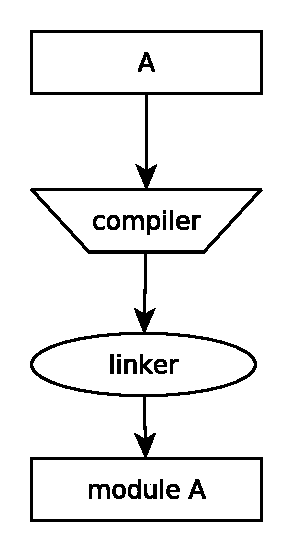
\includegraphics[width=0.20\linewidth]{figures/basic_module_compilation.pdf}
  \caption{Construction du module A à partir des sources.}
\end{figure}

%La création d'exécutable inclut deux étapes importantes, la compilation et
%l'édition des liens. La première étape consiste à prendre un fichier de code
%source et de le traduire en fichier objet, que l'on retrouve souvent avec
%l'extension \verb|.o| ou \verb|.obj|, qui contient la représentation des
%procédures compréhensible par le processeur. Ces fichiers objets ne sont pas
%encore exécutable pour autant, il faut tout d'abord effectuer la seconde étape,
%qui va les regrouper en un exécutable. Le programme qui s'occupe de l'édition
%des liens est le \textit{linker}, la version GNU se nomme \verb|ld|.  Voici
%l'exemple de la création d'un exécutable composé des fichiers sources C
%\verb|main.c| et \verb|foo.c|:
%
%\begin{figure}[ht]
%    \begin{minipage}[t]{0.5\textwidth}
%\begin{verbatim}
%# Compilation
%gcc -c main.c -o main.o
%gcc -c foo.c -o foo.o
%# Édition de liens
%ld -o main.exe main.o foo.o
%\end{verbatim}
%    \end{minipage}
%
%    \caption{Exemple de création d'un exécutable}
%\end{figure}


La construction d'un programme peut s'effectuer de façon modulaire; chaque
composantes du programme peuvent être construites en séparément.  La
modification d'une des bibliothèques partagés utilisés par
le programme ne nécessite pas la recompilation de celui-ci. Le nom qui est
donné à l'entité qui résout les noms des fonctionnalités est l'éditeur de liens (\textit{dynamic linker}).
Habituellement les bibliothèques exportent des fonctions, mais il peuvent aussi
exporter plusieurs types de données comme des entiers, des nombres à virgules,
des chaînes de caractères et des données composites (structures). Chacune de ces données est
associées à un nom unique (symbole) au sein de la bibliothèque.
Il n'est pas possible d'avoir deux bibliothèques statiques qui exportent une
fonctionnalité avec le même nom au sein d'une même application, alors qu'avec
les bibliothèques partagés c'est possible. Cela limite le choix des
bibliothèques qui peuvent être utilisé simultanément au sein du programme;
chaque bibliothèque doit avoir un ensemble de nom de fonctionnalité distinct
des autres. Puisque la résolution d'une fonctionnalité retourne la première
occurrence trouvée, il n'y a rien qui empêche d'avoir plus d'une fonctionnalité
associée au même nom.

Gambit permet de l'utilisation de bibliothèques statiques et dynamiques.
Chaque fichier Scheme peuvent être compilé et lié module exécutable ou
en bibliothèque dynamique.

\begin{center}
\begin{figure}[ht]
  \begin{tabular}{l}
    \begin{mplisting}{0.5}
;; fib.scm
(define (fib n)
  (if (< n 2)
      n
      (+ (fib (- n 1))
         (fib (- n 2)))))
\end{mplisting}
  \end{tabular}
  \caption{Un module qui implémente la fonction mathématique \texttt{fib}.}
  \label{fig:basic_fib_module}
\end{figure}
\end{center}

\vspace{-20pt}
La construction d'un bibliothèque dynamique à partir du fichier \texttt{fib.scm}
de la figure \ref{fig:basic_fib_module} s'effectue par le compilateur de Gambit
qui nomme \texttt{gsc}. Cela produit un fichier avec l'extension \texttt{.oN}
où le \texttt{N} correspond à la version généré de la bibliothèque qui commence à 1.


\section{Concepts}

% Définition sommaire d'une bibliothèque de code
Une bibliothèque de code est le regroupement de plusieurs types
de données, des entiers, des nombres à virgule flottant, des chaînes
de caractères, des fonctions et des données composites. L'ensemble
de ces données constitue les fonctionnalités de la bibliothèque.
Les fonctionnalités d'une bibliothèque peut être copié dans l'exécutable
(bibliothèque statique), cela facilité la distribution du binaire puisque
que ses dépendances sont inclus dans l'exécutable.
Les fonctionnalités d'une bibliothèque peuvent aussi être chargé
à l'exécution (bibliothèque partagés), cela permet de partagé des routine
commune entre plusieurs processus (programme en exécution). Les données de
la bibliothèque, par contre, ne sont partagé, chaque processus réfère à
sa propre version des données.
Le format d'une bibliothèque de code varie d'un langage à l'autre et aussi d'un
système d'exploitation à un autre. Les langages interprétés utilisent plus
souvent le code source directement ou une représentation intermédiaire comme format pour
les bibliothèques de code.
Pour les langages compilés, c'est le format natif correspondant au système d'exploitation
qui est le plus souvent utilisé. Le système d'exploitation Linux utilise le
format ELF (Extensible Linking Format), Microsoft Window utilise le format PE (Portable Executable)
et MacOSX utilise le format Mach-O (Mach object) pour les exécutables et les bibliothèques.
% XXX: bytecodes aussi pour les langage compilé.

%Les langages
%de programmation interprétés fournisse leurs bibliothèques directement
%en code source. Dans cette catégorie, il y a Ruby, Python, Perl, Lua et
%Scheme -- dont le code des bibliothèques est écrit et frounit dans le
%langage respectif. Les langages compilés -- comme C, C++, C\# et Java --
%utilisent plutôt des formats binaires destiné, soit à une machine virtuelle
%(e.g. la \textit{Java Virtual Machine} JVM ou un architecture
%physique (e.g. i686, x86\_64, ARM). Les bibliothèques natives peuvent
%être utilisé




Une application qui utilise une bibliothèque partagés ne contient pas le
code de la bibliothèque, mais plutôt le nom des fonctionnalités utilisés.
La routine qui permet de récupérer la fonctionnalité
à partir du nom est la résolution qui est effectué par le \textit{dynamic loader}.
Lorsqu'un programme lié dynamiquement
à plusieurs bibliothèques partagés exécute du code externe \verb|foo|,
un routine de résolution est démarré pour déterminé quelle bibliothèque
lié au fournit la fonctionnalité \verb|foo|.

%% Bibiothèque dynamique native.
Par exemple, sous Linux l'utilitaire <<yes>>, qui est écrit en C,
est lié aux bibliothèques systèmes suivantes:
\begin{verbatim}
  linux-vdso.so.1 (0x00007ffeef7f9000)
  libc.so.6 => /usr/lib/libc.so.6 (0x00007ff68161c000)
  /lib64/ld-linux-x86-64.so.2 => ...
\end{verbatim}
La bibliothèque \textit{libc.so.6} contient la plupart des fonctions
standards du système sous Linux dont les fonctionnalités sont résolut
à l'exécution.
% Le but d'une bibliothèque est la réutilisation de code.
Dans le contexte d'un exécutable natif, le chargement des bibliothèques
s'effectue au début de l'application, avant l'exécution de la fonction principale
souvent nommé \textbf{main}. Plusieurs bibliothèques peuvent coexister simultanément au
sein d'un même processus sans que l'exécution du programme en soit affecté.

La résolution des fonctionnalité de ces bibliothèques sont effectué par un programme adapté
le \textit{program interpreter} du système qui correspond à \textit{/lib64/ld-linux-x86-64.so.2}.
Il est possible de forcer la résolution d'une fonctionnalité d'une bibliothèque
de façon manuel. Ce genre d'interaction est possible sur
les trois principales plateformes utilisées sur le marché (Windows, MacOSX et Linux).

%% TODO: continue here FIXME
Sur Linux, l'API qui permet d'interagir avec les bibliothèques partagés provient de \textit{libdl.so}.
Elle contient les fonctions \textit{dlopen}, \textit{dlsym}, \textit{dlerror} et \textit{dlclose} pour gérer
des bibliothèques de code supplémentaire chargé manuellement à l'exécution.  Pour charger la fonction
\textit{foo}, qui ne prend pas d'argument et ne retourne rien de la bibliothèque \textit{libFoo.so} en C,
il faut exécuter les deux appels suivant:
\begin{center}
  \begin{figure}[ht]
\begin{lstlisting}[language=C,frame=single]
  ...
  void *handle = dlopen("./libFoo.so", RTLD_LAZY);
  void (*foo)() = dlsym(handle, "foo");
  ...
\end{lstlisting}
\caption{Chargement dynamique de la bibliothèque \textit{libFoo.so} et
résolution de la fonction \textit{foo} sans gestion d'erreur sous Linux}
  \end{figure}
\end{center}
L'équivalent des bibliothèques partagés sous Window sont les DLLs, ils peuvent être chargé de façon similaire dans un
programme en utilisant les fonctions \textit{LoadLibrary}, \textit{LoadLibraryEx} et \textit{GetProcAddress}. Ils
fonctionne de la même façon que leur équivalent Linux. Pour MacOSX, il faut passer par les routines:
\begin{itemize}
    \item \textit{NSCreateObjectFileImageFromFile}
    \item \textit{NSLinkModule}
    \item \textit{NSLookupSymbolInModule}
    \item \textit{NSAddressOfSymbol}
\end{itemize}

La majorité des langages interprétés permettent l'importation de bibliothèque de code natif, via un interface
nommé \textit{foreign function interface}.
Prenons comme exemple les langage Python, Ruby, Lua et Scheme. Python possède le module ctypes
qui permet de chargé des bibliothèques natives dynamique, Ruby possède le module ffi.
%Ces modules ne font qu'encapsuler les fonction de chargement de bibliotheques native pour qu'il puisse être invoqué
%dans le langage cible.

% Bibliothèque Lua en C
% - La bibliothèque doit avoir le même nom que celui utilisé par le \textit{import}.

Certains langages ont même un mécanisme pour charger des bibliothèques natives s'ils ont été conçus spécialement.
Dans le langage de programmation Lua, il est possible en Lua de chargé directement
une bibliothèque dynamique si elle contient une fonction principale \textbf{luaopen\_\textit{libname}}
où \textit{libname} est le nom de la bibliothèque.

Gambit Scheme utilise un mécanisme équivalent. Il permet le chargement de ces modules qui ont été compilé
en bibliothèque partagé (DLL) avec la fonction \textit{(\textbf{load} "libname")}. Le chargements de la
bibliothèque ressemble à celui de Lua.

%% Python
%\begin{figure}[ht]
%\begin{lstlisting}[language=python,frame=single]
%# From https://docs.python.org/2/library/ctypes.html
%from ctypes import *
%# Chargement d'une bibliotheque native.
%lib = cdll.LoadLibrary("./libFoo.so")
%# Appel de la fonction foo.
%lib.foo()
%\end{lstlisting}
%\caption{Code d'importation de la fonction \textbf{foo} de la bibliothèque \textit{libFoo.so} en Python}
%\end{figure}

\begin{center}
% Ruby
\begin{figure}[ht]
\begin{lstlisting}[language=ruby,frame=single]
require 'ffi'
# Chargement d'une bibliotheque native.
module LibFoo
    extend FFI::Library
    ffi_lib './libFoo.so'
    attach_function :foo, [], :void
end
# Appel de la fonction foo.
LibFoo.foo
\end{lstlisting}
\caption{Code d'importation de la fonction \textbf{foo} de la bibliothèque \textit{libFoo.so} en Ruby}
\end{figure}
\end{center}

La résolution des fonctionnalités effectué par le \textit{dynamic linker} utilise un ordre de recherche
définit. Cet ordre de recherche inclut l'exécutable courant, les dépendances de l'exécutable, la bibliothèque
passé à \textit{dlsym}. La résolution d'une fonctionnalité par \textit{dlsym} qui n'engendre pas la résolution
d'un autre fonctionnalité externe n'utilise pas le programme principale dans l'ordre de recherche qui alors
commence par la bibliothèque passé à \verb|dlsym| suivit de ses dépendances. Les résolution de fonctionnalité
provenant d'appels indirecte au \textit{dynamic linker} inclut le programme principal et ses dépendances avant
la bibliothèque passé à \verb|dlsym|.

\begin{center}
    \begin{figure}[ht]
        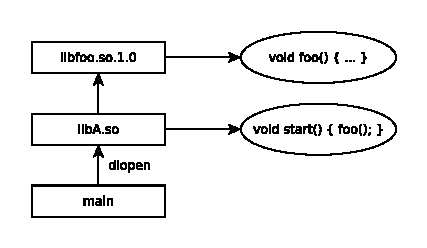
\includegraphics{figures/libdeps-ex1.pdf}
        \caption{Un exemple de dépendance de bibliothèques au sein d'un application simple fictive.
            La bibliothèque \textit{libA.so} est chargé dans l'application \texttt{main} via
            les appels au procédure \textit{dlopen} et \textit{dlsym}. Le fonctionnalités utilisés
            dans l'exemple sont marqué par un ellipse.
        }
        \label{fig:deps-ex1}
    \end{figure}
\end{center}

Dans la situation situation présenté dans la figure-\ref{fig:deps-ex1}, quels sont les étapes inclut
dans l'exécution de ce programme qui ne fait qu'appeler la fonctionnalité \texttt{start} de la
bibliothèque \textit{libA.so}. La fonctionnalité \texttt{start} est résolu de façon direct par
un appel à \verb|dlsym(libA, "start")|, qui commence la recherche de la procédure \texttt{start} dans
la bibliothèque spécifier dans \texttt{dlsym}. Le programme, une fois la procédure trouvé, l'exécute.
L'appel à une procédure non résolue (e.g.\ la procédure \texttt{foo} invoqué dans \texttt{start})
déclenche une procédure automatique de résolution des fonctionnalités. Cette procédure de résolution
commence sa recherche à partir de l'exécutable, puis itère la liste des dépendances directe. Si la
fonctionnalité n'est pas encore trouvé, la recherche continuera à partir de la bibliothèque passé à
\texttt{dlsym}.

% Stub

% TODO: exemple de résolution direct
Connaissant l'ordre de recherche du \textit{dynamic linker}, il est facile de construire un application avec des bibliothèques
qui cause un masquage de fonctionnalité. Deux possibilité facilement exploitable, faire que l'exécutable main fournisse
directement la fonctionnalité à masquer, ou avoir une des dépendances de l'exécutable contenant cette fonctionnalité. La figure-\ref{fig:deps-ex2}
en est l'exemple qui utilise la seconde méthode. La première consisterait à transformer l'exécutable main est bibliothèque
exécutable qui ne pourrait pas être supporté sur certaine plateforme. Sous Linux, il est possible de créer une bibliothèque qui
exécutable en passant le paramètre \texttt{-rdynamic} à \textit{gcc} lors de la construction.

\begin{center}
    \begin{figure}[ht]
        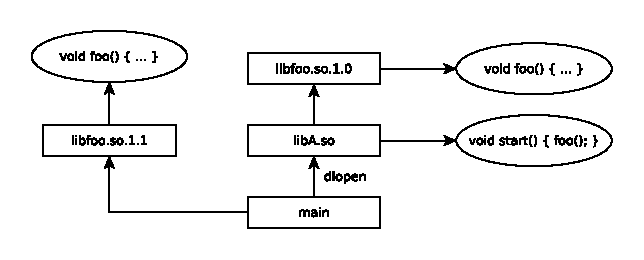
\includegraphics{figures/libdeps-ex2.pdf}
        \caption{Exemple de dépendance dans un application cause le masquage de la fonctionnalité \texttt{foo}
        de la bibliothèque \textit{libfoo.so.1.0} par la bibliothèque \textit{libfoo.so.1.1}}
        \label{fig:deps-ex2}
    \end{figure}
\end{center}
%% BEGIN
% D'autre langage compilé comme C/C++
% ne le permette pas directement, la liste des bibliothèques de code utilisé par un
% programme est déterminée lors de la création du fichier binaire, qui peut être
% soit un exécutable où une bibliothèque.
%% END


% TODO: pourquoi est-ce utile?
% XXX: structure pas final.
% - Les bibliothèques coexistent dans les application de tous les jours.
Analyser les interactions entre des bibliothèques au sein d'un même programme permet de
mieux comprendre quels sont les circonstance qui peuvent conduire à des comportements
non désirés, par exemple le masquage démontré dans la figure-\ref{fig:deps-ex2}.
Cela permet aussi d'établir les conditions qui inhibe ces comportements non désirés.

%Cela implique que ils possible de retrouvé une dépendance en diamant tel que représenter
%dans la figure-\ref{fig:dep1} qui peut causer un problème. % Détailler
%\begin{figure}[ht] %% Pas juste valide pour scheme.
%  \begin{center}
%    %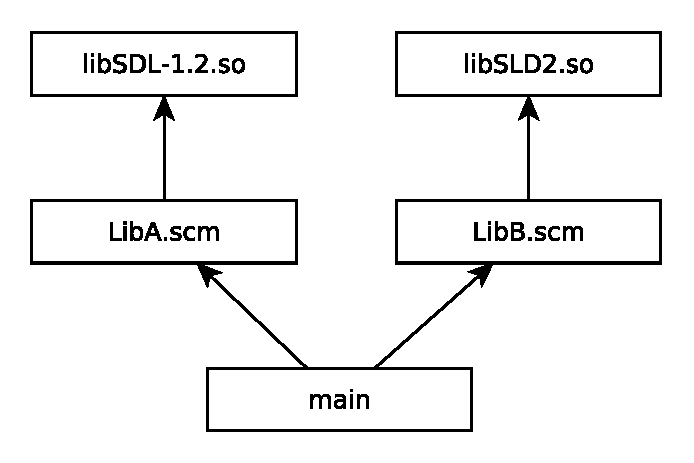
\includegraphics[width=4cm]{figures/SchemeLibrary}
%    \caption{Dépendence en diamant}
%    \label{fig:dep1}
%  \end{center}
%\end{figure}

%% NOTE: Soit P un processus, execution(A, P=[A,B]) == execution(A, P=[A]).
%Soit un processus \textbf{P} qui réfère aux bibliothèques \textbf{A} et \textbf{B}.
%Une bibliothèque peut masquer les symboles d'une autre bibliothèque chargé dans le même processus.
%La bibliothèque \textbf{A} coexiste avec la bibliothèque \textbf{B} si la \textbf{A}
%ne masque pas des symboles ne \textbf{B} qui amène un comportement non défini.


% Historiquement, il y avait un problème avec la coexistence entre deux dll sous Window. TODO: devellopper

% - Système distribué (Actor), non limité par la diversité des bibliothèque.


% TODO:
%La coexistance entre plusieurs versions d'une même bibliothèque
%===========================================================
%
% - Définition d'une bibliothèque
%   - Nom symboles:
%     - Fonction
%     - Variables global
%     - Structure de donnée
%     - Macro (Compilation)
%
%- Définition par coexistence de plusieurs bibliothèque.
%- Pourquoi est-ce utile?
%- Conditions nécessaire pour la coexistence entre plusieurs versions d'une même bibliothèque soit possible.
%  - Data race.
%  - État partagé.
%- Système d'exploitation (DOS)




\chapter{Bibliothèque Scheme}

Le langage Scheme\cite{Scheme} à été conçu en 1975 par Guy L. Steele et Gerald
Jay Sussman.  C'est un langage de programmation avec un système de type
dynamique, cela signifie que les variables peuvent contenir n'importe quels
types. Il supporte plusieurs paradigmes de programmation comme fonctionnelle,
impérative et méta. Chaque expression est représenté sous forme préfixé et
fortement parenthésé.  Un programme Scheme est une séquence de liste parenthésé
en forme préfixé, ce sont des \textit{s-expresssions}.  Chaque
\textit{s-expression} correspond soit à une constante, une application de
procédure ou une application de macro. Les macros sont lié au paradigme de
méta programmation qui manipulent les expressions.

Les formes de base usuelles en Scheme sont \lstcode{define}, \lstcode{lambda},
\lstcode{let}, \lstcode{if} and \lstcode{set!}.
\begin{itemize}
  \item La forme \lstcode{(define <name> <val>)} associe le nom \lstcode{<name>} avec
    la valeur \lstcode{<val>}. Il est utilisé pour définir des variables globales.

  \item La forme \lstcode{(lambda <args> <body>)} permet la définition de
    procédures anonymes. Les arguments sont \lstcode{<args>} et le corps
    de procédure \lstcode{<body>}.

  \item La forme \lstcode{(let <bindings> <body>)} permet de créer des
    associations (\lstcode{<bindings}) visible seulement dans le contexte de
    \lstcode{<body>}. Les associations sont sous la forme d'une liste
    associative nom et valeur.

  %% XXX: Too much???
  \item Les conditions sont géré par la forme \lstcode{(if <e1> <e2> <e3>)}.
    La branche \lstcode{<e1>} est exécutée si la condition \lstcode{<e2>} est
    vrai sinon \lstcode{<e3>}.

  \item La forme \lstcode{(set! <name> <val>)} modifie le contenu de la variable
    \lstcode{<name>} avec la valeur \lstcode{<val>}.
\end{itemize}

%read from here

La méta programmation est un paradigme lié à l'utilisation de macro qui sont
des entités qui manipulent la structure du programme. Elle est utilisé pour
ajouter des abréviations dans le langage qui simplifie l'écriture du code.  La
section \ref{sec:proc_and_macro} détaille de la méta programmation en Scheme.

Les expressions Scheme sont en forme préfixe. Cela signifie que l'opération
précède les opérandes. Cette forme est plus utilisé dans les langage de la famille
LISP.

% Une expression peut être organisé de plusieurs façons, infixe, préfixe ou
% suffixe.  La différence entre ces organisations est l'emplacement de
% l'opération et des opérandes dans l'expression.  Une expression en syntaxe
% infixe place l'opération entre les opérandes.  Cette forme est souvent utilisé
% dans les langages impératif. La forme préfixe commence par l'opérateur suivie
% des opérandes. Cette forme est plus utilisé dans les langages de la famille
% LISP.  La forme suffixe place les opérations après les opérandes.  Le tableau
% \ref{tab:prefix_vs_infix} donne des exemples d'expression préfixe avec
% l'équivalent infixes.


% \begin{verbatim}
% - Scheme
%    - Langage dynamique
%   - Supporte plusieurs paradigmes:
%     - fonctionnel
%     - impérative
%     - méta (programmation de macro)
%   - Préfixé / ~Infixe
%   - S-expression
% \end{verbatim}


\begin{table}[htbp]
\begin{center}
\begin{tabular}{|l|l|l|}
  \hline
  \textbf{Préfixe}& \textbf{Infixe}& \textbf{Suffixe}\\\hline
  \begin{mplisting}{0.1}
(+ 1 2)
\end{mplisting}&
  \begin{mplisting}{0.1}
1 + 2;
\end{mplisting}&
  \begin{mplisting}{0.1}
1 2 +
\end{mplisting}\\
\hline
  \begin{mplisting}{0.22}
(proc a1 a2 a3)
\end{mplisting}&
  \begin{mplisting}{0.22}
proc(a1, a2, a3);
\end{mplisting}&
  \begin{mplisting}{0.22}
a1 a2 a3 proc
\end{mplisting}\\
\hline
%    \begin{mplisting}{0.25}
%(if e1
%    e2
%    e3)
%\end{mplisting}&
%    \begin{mplisting}{0.25}
%if(e1)
%  e2;
%else
%  e3;
%\end{mplisting}\\
%\hline
\end{tabular}
\end{center}
  \caption{Voici des example qui montre une comparaison entre une syntaxe préfixe, infixe et suffixe.}
  \label{tab:prefix_vs_infix}
\end{table}

% La définition des associations globales en Scheme est effectuée avec \lstcode{define}.

Les différents types que les valeurs peuvent prendre sont Les types de donnée
disponible en Scheme sont \lstcode{boolean}, \lstcode{pair}, \lstcode{symbol},
\lstcode{number}, \lstcode{char}, \lstcode{string}, \lstcode{vector},
\lstcode{port} et \lstcode{procedure}.

\section{Procédure et Macro}
\label{sec:proc_and_macro}

Les procédures sont des objets de premier classe, cela signifie qu'elles
peuvent être manipulée comme n'importe quels types de donnée. Elles peuvent
être passées en tant que paramètre à une procédure et retourné en tant que
résultat.  Certaines fonctions -- telles que \lstcode{map}, \lstcode{fold}, etc.
-- bénéficie que les procédures sont des objets de premier classe.

Les procédures et les fonctions sont définis par le constructeur
\lstcode{lambda} qui prend une liste d'arguments et une séquence d'au moins une
\textit{s-expression} comme corps. Lors de l'application d'une procédure chacun
des arguments est évalué puis passés à la procédure. C'est un mode de passage
de paramètre par valeur. Il n'y a de forme spéciale pour les boucle, car elle
peuvent construite par la récursion. Le langage offre une récursion sans coût
avec l'appel terminal.  Il est possible d'ajouté une syntaxe pour les boucle en
utilisant la méta programmation.
% forme spéciale pour les boucle -> Les boucles sont faite par la récursion


% \begin{figure}[ht]
%   \begin{center}
%     \begin{tabular}{|l|}
%       \hline
%     \begin{mplisting}{0.55}
% (define fact
%   (lambda (n) (if (= n 0) 1
%                   (* n (fact (- n 1))))))
% \end{mplisting}\\\hline
%     \end{tabular}
%   \end{center}
%   \label{fig:fact1}
%   \caption{Voici une implémentation de la fonction factoriel en Scheme.
%   Cela montre un exemple de récursion.}
% \end{figure}

% READ Distinguer macro procedure.
% \begin{figure}[ht]
%   \begin{center}
%     \begin{tabular}{|l|}
%       \hline
%     \begin{mplisting}{0.65}
% (define map
%   (lambda (f lst)
%     (if (pair? lst)
%         (cons (f (car lst)) (map f (cdr lst)))
%         lst)))
% \end{mplisting}\\\hline
%     \end{tabular}
%   \end{center}
%   \label{fig:fact1}
%   \caption{Voici une implémentation de la fonction d'ordre supérieur \lstcode{map} en Scheme.
%   Cela montre un exemple utilise les procédure en objets de première classe et
%   aussi un exemple d'application récursive.}
% \end{figure}



% La récursion est la façon dont les boucle sont faites.
La programmation méta est présente dans plusieurs langage comme C, C++, LISP,
Haskell, Scheme, etc. Elle est basé sur la capacité d'un programme de manipuler
d'autre programme comme des données. Cela implique qu'il est possible de
générer, analyser et modifier le code d'un autre programme s'incluant.  Les
constructions utilisées pour manipuler le code du programme et
ajouter des extensions au langage sont les macros.

En C et C++, les macros ne permettent pas de récursion se référant à elle-même.
Ils sont basés sur un modèle de remplacement textuel simple. Un appel à la
macro est remplacer par le corps de celle-ci. Les macros de style LISP ont
accès à l'ensemble des procédure, ce qui leurs donne plus de flexibilité.  La
différence entre les procédures et les macros est le mode de passage de
paramètres.  Les paramètres sont passés à la macro sans être évalués, c'est ce
qu'on appelle le passage par nom.  Certain Scheme offre la forme
\lstcode{define-macro} pour définir les macros.  Cette forme est équivalente au
\lstcode{defmacro} de LISP. Elle accepte en entré des \textit{s-expression}s et
retourne une \textit{s-expression} (soit une liste ou une constante).  Le
problème de cette forme spéciale est l'hygiène qui est traité dans le chapitre
\ref{XXX}.

\begin{figure}[htbp]
  \begin{tabular}{|l|}\hline
\begin{mplisting}{0.7}
(define-macro (include filename)
  (call-with-input-file
    filename
    (lambda (port)
      `(begin
        ,@(read-all port)))))
\end{mplisting}\\\hline
\end{tabular}

  \caption{Implémentation de la macro \texttt{include} qui permet l'inclusion
  d'un fichier dans un autre fichier avec la syntax \texttt{define-macro}.}

  \label{fig:macro_include}
\end{figure}

Un exemple qui montre les capacité des macros Scheme est la macro
\lstcode{include}.  Cette macro permet l'inclusion du contenu d'un fichier au
point d'application.  Pour inclure un fichier dans un autre, il faut tout
d'abord lire le contenu du fichier à inclure. Ensuite, il suffit de retourné le
code lu. La figure \ref{fig:macro_include} montre une implémentation de cette
macro avec \lstcode{define-macro}.  Pour les implémentation de Scheme ne
supportant pas la forme \lstcode{define-macro}, il est possible d'implémenter
la forme \lstcode{include} avec \lstcode{define-syntax} qui est l'alternative à
\lstcode{define-macro}. L'implémentation de cette macro est donnée à la figure
\ref{fig:macro_include_def_syntax}. Les particularité de
\lstcode{define-syntax} ne sont pas mentionnées dans ce mémoire.

% --------------------------------------MOVE--------------------------------------

% Certaines implémentations de Scheme n'ont pas la forme
% \lstcode{define-macro}. Il est possible d'écrire la macro
% \lstcode{include} en utilisant la \lstcode{define-syntax}
% et \lstcode{syntax-case} qui fait partie du standard R5RS
% \cite{Scheme:R5RS}. La figure \ref{fig:macro_include_def_syntax}
% montre implémentation possible de cette macro.

\begin{figure}[ht]
\begin{tabular}{|l|}\hline
\begin{mplisting}{0.8}
(define-syntax include
  (lambda (stx)
    (define (read-all port)
      (let loop ((rev-lst '()))
        (let ((expr (read port)))
          (if (eof-object? expr)
            (reverse rev-lst)
            (loop (cons expr rev-lst))))))
    (syntax-case stx ()
      ((_ fn)
       (let ((filename (syntax->datum (syntax fn))))
         (let ((content
                 (call-with-input-file
                    filename
                    (lambda (port)
                      (cons 'begin (read-all port))))))
           (datum->syntax stx content)))))))
\end{mplisting}\\\hline

\end{tabular}
   \caption{Implémentation de la macro \texttt{include} qui permet l'inclusion
   d'un fichier dans un autre fichier avec la syntaxe \texttt{define-syntax}.
   Cette macro effectue la même action que celle définit dans la figure
   \ref{fig:macro_include}.}

   \label{fig:macro_include_def_syntax}
\end{figure}

\section{Structure des Bibliothèques}

Les bibliothèques, aussi appelées modules, facilitent le partage de
fonctionnalités entre plusieurs programmes. Dans le standard
R4RS\cite{Scheme:R4RS} et R5RS\cite{Scheme:R5RS} les modules consistent en des
fichiers Scheme qui contiennent des définitions de procédures et de macros. Il
sont chargés dans le module courant par la procédure \lstcode{load}. Certaines
implémentations de Scheme ont la forme spéciale \lstcode{include} qui permet de
séparer un module Scheme en plusieurs parties. Cette forme peut s'ajouter
facilement au langage (voir la figure \ref{fig:macro_include_def_syntax}).  Le
modèle de bibliothèque de la 4e et 5e révision de Scheme possède plusieurs
lacunes.

%% Gambit doc
\begin{itemize}
  \item Ce modèle de chargement n'est pas à l'abri des chargements multiples
    d'un module qui mène soit à de la duplication de code (dans le cas de \lstcode{include})
    ou à de la réévaluation d'un code (dans le cas de \lstcode{load}).

  \item Toutes les déclarations dans un module sont ajoutés à l'environnement
    global lors du chargement par \lstcode{load}. Cela mène à des conflits de
    nom entre les identifiants du module principal et des modules importés.

  \item L'importation d'un module par \lstcode{load} ou \lstcode{include} nécessite la connaissance
    de son emplacement dans le système de fichier. L'emplacement spécifier est soit relatif ou
    absolu.

\end{itemize}

% \begin{verbatim}
% +-----------------------------------+
% | - Analyse lexicale                |
% | - Analyse syntaxique              |
% | - Expansion macro                 |
% | - Evaluation                      |
% +-----------------------------------+
% \end{verbatim}

Le chargement d'un module dans Gambit Scheme par \lstcode{load} se fait en plusieurs
phases: l'analyse lexicale, l'analyse syntaxique, l'expansion de macro et
l'évaluation. L'analyse lexicale brise l'expression en mots. La séquence de
mots est associée à un contexte par l'analyse syntaxique dans laquelle il y a aussi
une expansion des macros. Le \lstcode{include} d'un fichier n'effectue qu'un
analyse lexicale qui est effectué par la procédure \lstcode{read}. L'évaluation
est effectué après l'analyse syntaxique et l'expansion des macros. D'autres systèmes
Scheme permettent le chargement des macros par \lstcode{load}.

Dans un module, il y a du code qui est exécuté lors de l'expansion (les macros)
et à l'évaluation. La procédure \lstcode{load} donne accès au procédure définit
dans le module, mais pas aux macros, car elles sont expansées.  Après un
\lstcode{load}, il ne reste que les procédures et variables globales qui
résultent de l'expansion des macros.  Pour avoir accès aux macros, il faut
utiliser la forme spécial \lstcode{include} qui est expansé par le contenu du
fichier.  L'expression \lstcode{(include "foo#.scm")} est remplacé par le
contenu du fichier \lstcode{foo#.scm}. L'exemple \ref{fig:r4rs_fact} montre un
exemple de module simple n'utilisant que \lstcode{load}.

\begin{figure}[ht]
  \begin{center}
    \begin{tabular}{|l|l|}
    \hline
    \begin{mplisting}{0.4}
;; fact.scm
(define (fact n)
  (if (< n 2)
    n
    (* n (fact (- n 1)))))
\end{mplisting} &
    \begin{mplisting}{0.4}
;; main.scm
(load "fact.scm")
(display (fact 5))
\end{mplisting} \\\hline
    \end{tabular}
  \end{center}

  \caption{Le fichier \texttt{fact.scm} est un exemple de module R4RS exposant
  la fonction mathématique \lstcode{fact}. Le fichier \texttt{main.scm} est un
  programme principal qui utilise le module \texttt{fact.scm}.}
  \label{fig:r4rs_fact}
\end{figure}


% - Structure global
% - Nom module
% - Export
% - Import
% - Corps de module

Le standard R6RS\cite{Scheme:R6RS} renforce le concept de modules avec la
syntaxe \lstcode{library}.  Un module R6RS est séparé en 4 parties: le nom, une
sous forme \lstcode{export}, une sous forme \lstcode{import} et le corps du
module. Le nom du module l'identifie de façon unique, il peut contenir une
spécification de version. La version est spécifié par une liste d'entiers
positifs. Une liste vide \lstcode{()} est l'équivalent de ne pas spécifier la
version. Ensuite, il y a la liste des exportation spécifier par la sous forme
\lstcode{export}. Chaque élément de cette liste est soit un identifiant ou un
une sous forme \lstcode{rename} qui renomme l'identifiant exporté. Le
\lstcode{import}, donne la liste des dépendances du module. Chaque dépendance
spécifie:

\begin{itemize}
  \item le nom du module importé et de façon optionnelle une contrainte sur
    la version;
  \item le niveau d'import (temps d'expansion ou évaluation);
  \item un sous ensemble du \lstcode{export} du module et le nom local
    utilisé au sein du module courant pour chaque exportation du module.
\end{itemize}

Le corps du module contient une séquence de définitions suivit par une séquence
d'expressions. Une définition peut être soit local ou exportée. Les expressions
initialisent le module lors de l'exécution.  Le R6RS ajoute aussi la forme
\lstcode{import} pour l'importation d'un module et enlève la procédure
\lstcode{load}.  Contrairement au \lstcode{load}, la forme \lstcode{import}
empêche le chargement multiple d'un module.  La syntaxe du \lstcode{import}
permet de manipuler les noms des symboles importés et exportés.\\
\begin{center}
  \lstset{language={scheme},
          captionpos=b,
          caption={Structure globale d'un module R6RS}}
  \begin{mplisting}{0.5}
(library <library name>
  (export <export spec> ...)
  (import <import spec> ...)
  <library body>)
\end{mplisting}
\end{center}

La forme \lstcode{import} de R6RS permet l'importation d'un ensemble de module.
Chaque spécification d'import \lstcode{<import spec>} peut être soit une simple
importation ou un importation avec un niveau. Le niveau d'importation est soit:
\lstcode{run}, \lstcode{expand} ou \lstcode{(meta <level>)}.  Le niveau méta
donné par \lstcode{<level>} est un entier exacte. Un niveau d'importation 0
correspond à \lstcode{run} et un niveau d'importation de 1 correspond
\lstcode{expand}.

% L'importation d'un module contient les sous formes suivantes:
% \begin{center}
% \begin{mplisting}{0.7}
%   <libref>
%   (library <libref>)
%   (only <import set> <identifier_1> ...)
%   (except <import set> <identifier_1> ...)
%   (prefix <import set> <identifier>)
%   (rename <import set> (<identifier_1> <identifier_2>))
% \end{mplisting}
% \end{center}

% \begin{itemize}
%   \item \lstcode{(rename  (<identifier1> <identifier_2>))}
% \end{itemize}

La syntaxe pour l'importation avec les niveau méta est décrit dans la
spécification R6RS~\cite{Scheme:R6RS}. Le \lstcode{import} R6RS permet un grand
contrôle lors de l'importation des modules au prix d'une sémantique plus complexe.

Les déclarations d'un module R6RS sont dans espace distinct de l'espace global et
des autres modules. Les déclarations d'un module ne peuvent pas être en conflit avec
des déclaration global ou d'autre module. L'élément qui distingue deux module est
son nom avec sa version. Le nom du module correspond à l'espace de nom du module.
C'est ce qui lie les déclarations au module et empêche les conflits de nom entre
les modules.


%Cette syntaxe
%est fortement lié à ce module. Chaque module a son propre
%espace de environnement. dans l'espace de nom du module sert d'espace de nom pour les associations
%du module. Ce modèle introduit le concept d'espace de nom
%qui donne l'appartenance des fonctionnalités à un module. Cela règle le
%problème que module redéfinisse les fonctionnalités d'un autre module.


% Le concept de bibliothèque a été raffiné  dans le R6RS.  Le R6RS rend le
% support de la procédure \texttt{load} optionnel et ajoute une forme spéciale
% \texttt{library} pour définir des bibliothèques et une autre forme spéciale
% \texttt{import} pour gérer la inclure une bibliothèque.  Les noms utilise
% pour nommer une bibliothèque peuvent seulement contenir des symboles et des
% numéros de versions à la fin. Les expression import et export doivent seulement
% apparaître une seul fois dans le définition de la bibliothèques.

% Les bibliothèques ainsi définit, lie chaque définitions à la bibliothèque.  Cela
% permet la réutilisation des mêmes identificateurs dans deux bibliothèque
% différente.  Les conflits de nom sont gérés lors de l'importation des la
% bibliothèques. L'importation d'un module est permit au sein d'une bibliothèque
% comme dans un programme principale. La syntaxe d'un import reste identique dans
% ce deux cas.

% Pour évité ces conflit, il faut que tous les noms utilisés au sein des
% bibliothèques soit distinct, ce qui ajoute une tâche au programmeur.

% What is define-library?
Le standard R7RS\cite{Scheme:R7RS} simplifie la syntaxe des modules
R6RS\cite{Scheme:R6RS}.  L'importation d'un module fait abstraction du niveau
d'importation. Les macros et les procédures sont importés de façon
transparente. La procédure \lstcode{load} est conservée. La forme spéciale pour
définir un module est \lstcode{define-library}. Il n'y a pas d'ordre spécifique
dans les déclarations de la bibliothèque comme en R6RS. Un module R7RS commence par
un nom suivit de plusieurs déclarations.\\
\begin{center}
  \lstset{language={scheme},
          captionpos=b,
          caption={Structure globale d'un module R7RS},
          label={lst:syntax->define-library}}
  \begin{mplisting}{0.5}
(define-library <library name>
  <library declaration>*)
\end{mplisting}
\end{center}

Une déclaration dans un module est soit un \lstcode{import}, un \lstcode{export},
un \lstcode{include}, un \lstcode{include-ci}, un \lstcode{cond-expand} ou un
bloque \lstcode{begin}.
\begin{itemize}
  \item La déclaration \lstcode{import} est équivalent au R6RS sans le concept
    de niveau d'importation.

  \item La déclaration \lstcode{export} est idem au R6RS.

  \item Les déclarations \lstcode{include} et \lstcode{include-ci} permettent
    l'inclusion d'un fichier en tant qu'un bloque de code.  La seconde version
    non sensible à la casse des caractères.

  \item La déclaration \lstcode{cond-expand} est un extension du \texttt{SRFI-0}
    dans le contexte d'une bibliothèque.

\end{itemize}

La forme \lstcode{import} en R7RS permet d'importer un ensemble d'identifiants
qui sont exporté par un module. Chaque ensemble importé spécifie le nom des
identifiants du module et parfois même associe un nom local aux identifiants.
Le \lstcode{import} peut prendre l'une des formes suivante:
\begin{itemize}
  \item \lstcode{<library-name>}
  \item \lstcode{(only <import-set> id1 ...)}
  \item \lstcode{(except <import-set> id1 ...)}
  \item \lstcode{(prefix <import-set> id)}
  \item \lstcode{(rename <import-set> (id1 id2) ...)}
\end{itemize}


--------------------------------------END---------------------------------------\\


% L'implémentation des bibliothèques Scheme est basé sur le standard R7RS qui
% conserve la procédure \texttt{load} que le R6RS enlève et remplace la structure
% des bibliothèques.  Une bibliothèque en R7RS remplace la forme
% \lstcode{library} par \texttt{define-library}. Ces deux formes ont beaucoup de
% similarité, il existe une méthode pour transformer certaines bibliothèques R6RS
% en bibliothèques R7RS. Takashi Kato a publié un article au \emph{Scheme
% Workshop} 2014 qui explique une procédure pour écrire un module R6RS en R7RS
% \cite{SW2014:R6RS/on/R7RS}.  L'extension de fichier utilisé par les définitions
% des bibliothèques est \verb|.sld| qui signifie \emph{Scheme Library
% Declaration}.

\begin{center}
  \begin{figure}[h]
  \begin{tabular}{|l|l|}
    \hline
    \begin{mplisting}{0.5}
;; Library R6RS
(library (math)
  (export fact)
  (import (rnrs base))
  (define (fact n)
    (if (< n 2)
      1
      (* n (fact (- n 1))))))
\end{mplisting} &
    \begin{mplisting}{0.5}
;; Library R7RS
(define-library (math)
  (export fact)
  (import (scheme base))
  (begin
    (define (fact n)
      (if (< n 2)
        1
        (* n (fact (- n 1)))))))
\end{mplisting}\\\hline
  \end{tabular}
    \caption{Comparaison entre la syntaxe des modules R6RS et R7RS}
% \caption{À gauche, il y a un exemple d'une bibliothèque mathématique dans le format R6RS qui implémente
% la fonction factoriel. À droite, une réécriture de la bibliothèque de gauche en R7RS.}
  \label{fig:r6rs_r7rs_math_mdoule}
\end{figure}
\end{center}

La syntaxe \lstinline{import} définit dans le R7RS indique le nom de
de la bibliothèque à collecter en plus des information sur les composante
à importer.
\begin{figure}[ht]
  \begin{mplisting}{0.9}
(import (only (gambit thread) make-thread thread-start! thread-join!))
\end{mplisting}
  \caption{Importation d'un sous-ensemble des fonctionnalité de la bibliothèque}
\end{figure}

% - (import (foo)) ; exportant f1 f2 f3
% ===>
% - (##demand-module foo)
% - (##namespace ("foo") f1 f2 f3)
% - macros
% - (##namespace (""))



%% ---- MOVED to chapter 4 ----

%\section{Chargement des bibliothèques}

%Un système est composé d'un ensemble d'éléments (modules) qui interagissent
%entre eux.  Une bibliothèque fait office de module au sein d'un système simple
%ou complexe.
%%La collection des modules s'effectue au sein d'un

%% TODO: voir chargé
%Le chargement d'une bibliothèque Scheme (ou module) est séparé en plusieurs niveaux.
%% TODO: later
%Les bibliothèques sont soit lu du disque vers la mémoire durant l'exécution
%ou déjà dans la mémoire du processus. Durant la compilation les modules sont
%collecté pour construire un exécutable. Le chargement
%d'une bibliothèque inclut une phase de recherche sur le système de fichier pour valider
%l'existence de la bibliothèque et des fonctionnalités demandés. L'emplacement des
%bibliothèques sur le système de fichier est lié par défaut aux chemin spécifié par
%le \lstinline{##module-search-order} a comme défaut \lstinline{~~lib} et \lstinline{~~userlib}.


%La procédure exacte de chargement des bibliothèques par \verb|import|
%n'est pas spécifier par le standard R7RS. Le standard spécifie seulement la syntaxe
%à utilisé et le de comportement principal qui est
%requis. L'importation d'une bibliothèque doit chargé la bibliothèque
%et rendre c'est fonctionnalité disponible dans le contexte
%l'importation a eu lieu qui peut soit ovenir d'un programme principale
%ou d'une bibliothèque.

%Le chargement d'une bibliothèque peut-être effectuée à l'exécution par
%l'utilisation de \texttt{eval} (par \texttt{load}) pour les fichiers source et
%\texttt{load-objcet-file} pour les bibliothèques compilées. Cette recherche
%peut aussi avoir lieu durant l'édition des lien en utilisant les méta-infos
%contenus dans les \textbf{.c} qui sont chacun compilé par le compilateur C
%en \textbf{.o} et lié par le \textit{linker}.

%\section{Modèle dynamique}
%Dans ce modèle les bibliothèques sont lié au programme durant l'exécution. Cela
%nécessite que les bibliothèques soit organisé sur le système de fichier d'une façon
%distingable. Chaque module doit posséder un nom unique qui permet d'y référer.
%Ce nom unique va être utilisé lors de la collection des dépendances.


%%Les bibliothèques
%%sont soit en code source ou compilé nativement avec l'extension (\textit{.oN})
%%où le N correspond à la version du binaire qui commence à 1.


%La recherche des bibliothèques est effectué dans un ordre spécifique
%indépendant de la spécification.  L'algorithme de recherche les bibliothèques
%prend entré le nom de la bibliothèque et retourne le chemin absolu
%correspondant à sont emplacement dans l'arborescence du système de fichier. Les
%bibliothèques sont situées dans différents répertoires l'origine du programme,
%le répertoire des bibliothèques système (\lstinline{~~lib}) et le
%répertoire de bibliothèque utilisateur (\lstinline{~~userlib}).

%% \begin{itemize}
%%   %% XXX: directory where the executable is located (usefull for devel no need to install the module). collecté
%%   \item \verb|origin/dummy.sld|
%%   \item \verb|origin/dummy/dummy.sld|
%%   \item \verb|~~userlib/dummy.sld|
%%   \item \verb|~~userlib/dummy/dummy.sld|
%%   \item \verb|~~lib/dummy.sld|
%%   \item \verb|~~lib/dummy/dummy.sld|
%% \end{itemize}

%Chaque module possède trois niveau d'initialisation dans le système numéroté de
%0 à 2. Le niveau 0 indique que le module n'a pas été initialisé. Ces les niveau
%des module qui ont juste été collecté par le système. Le niveau 1 indique que
%le descripteur du module à été récupéré. L'étape 2 est utilisé pour indiquer
%les module chargé.

%Soit un système avec les dépendance suivante:
%\begin{figure}[ht]
%  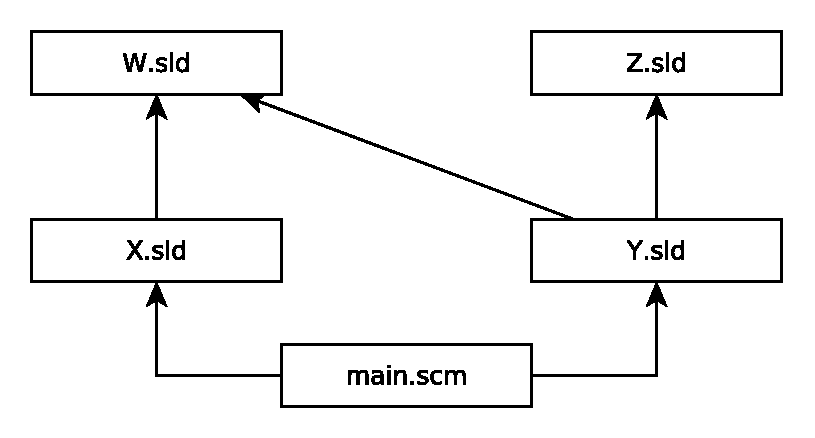
\includegraphics{figures/system-example}
%  \caption{Un exemple d'un système fictif composé de différents modules.
%  Le module principale se nomme utilise l'extension \textbf{.scm}
%  et les bibliothèques porte l'extension \textbf{.sld}}
%\end{figure} % TODO: use yed for that graph


%Le démarrage du module principal Main.scm déclenche la collection des modules X
%et Y, qui récursivement déclenche la collection de W et Z. L'algorithme de
%collection des modules ignore les module qui apparaisse plusieurs fois au sein
%du graphe.

%Une fois la collection de tous ces modules est complété le descripteur de
%module est récupéré par un appels à \verb|dlopen| et \verb|dlsym| dans le cas
%compilé.


%\section{Module hébergé}

%Un module qui est hébergé est un module qui dont son contenu
%se retrouve sur un domain comme \url{github.com}.


%\begin{figure}[ht]
%\begin{lstlisting}
%hostname      = +( domainlabel "." ) toplabel
%domainlabel   = alphanum | alphanum *( alphanum | "-" ) alphanum
%toplabel      = alpha | alpha *( alphanum | "-" ) alphanum
%alphanum      = alpha | digit
%alpha         = [a-zA-Z]
%digit         = [0-9]
%\end{lstlisting}
%  \caption{Grammaire BNF représentant un hostname selon un sous
%  ensemble du RFC-2396.}
%\end{figure}

%La différence avec la spécification du hostname dans le RFC-2396
%est que le hostname ne peut pas finir par un point et doit contenir
%au moins un \verb|domainlabel|. C'est pour permettre de distingué
%un module local et un module hébergé.

%\subsection{Module gambit/git}

%Ce module offre un interface pour utiliser interagir avec les des dépôts git.
%Il permet de cloner un dépôts qui est hébergé sur \url{github.com}. Un clone du
%dépôts est simplement un copie qui contient les informations suffisantes pour
%passer d'une version d'un module à un autre. L'opération qui permet de changer
%de version est \emph{checkout}.


%%-------------------------------------------------------------------------------
%%
%%Modèle "link dynamique" :
%%  recherche des libs au run time, utilisation de eval (par load) et
%%  load-object-file
%%
%%  % gsi main.scm      ou      % gsc main.scm ; gsi main.o1
%%
%%    origin/main.scm    : (import X Y)
%%          /X/X.sld     : (import)
%%
%% ~~userlib/Y/Y.sld     : (import Z)
%%
%%     ~~lib/Z/Z.sld     : (import)
%%          /Z.o1
%%
%%-------------------------------------------------------------------------------
%%
%%Modèle "link statique" :
%%  recherche des libs au link time en utilisant les méta-infos
%%  dans les .c (demand-lib et supply-lib), chaque .c compilé en
%%  un .o séparément et les .o linkés par le compilateur C
%%
%%  % gsc -obj -keep-c X.sld      ;; créer .c et .o
%%  % gsc -obj -keep-c Y.sld      ;; créer .c et .o
%%  % gsc -obj -keep-c Z.sld      ;; créer .c et .o
%%  % gsc -obj -keep-c main.scm   ;; créer .c et .o
%%  % gsc -exe main.c             ;; combine les .o pour créer main.exe
%%
%%    origin/main.scm    : (import X Y)
%%          /main.c      : (demand-lib X Y)
%%          /main.o
%%          /X/X.sld     : (import)
%%            /X.c       : (demand-lib) (supply-lib X)
%%            /X.o
%%
%% ~~userlib/Y/Y.sld     : (import Z)
%%          /Y/Y.c       : (demand-lib Z) (supply-lib Y)
%%          /Y/Y.o
%%
%%     ~~lib/Z/Z.sld     : (import)
%%          /Z/Z.c       : (demand-lib) (supply-lib Z)
%%          /Z/Z.o
%%
%%-------------------------------------------------------------------------------
%%
%%Modèle "whole-program" :
%%  recherche des libs au compile time en utilisant les imports
%%  dans les fichiers sources, les AST de toutes les libs fusionnées
%%  en un seul AST compilé par gsc (donc un seul .c généré et compilé
%%  par le compilateur C pour créer main.exe)
%%
%%  % gsc -exe -whole-program main.scm
%%
%%    origin/main.scm    : (import X Y)
%%          /X/X.sld     : (import)
%%
%% ~~userlib/Y/Y.sld     : (import Z)
%%
%%     ~~lib/Z/Z.sld     : (import)
%%
%%-------------------------------------------------------------------------------
%% correction d’une petite coquille…
%% /Y.c       : (demand-lib Z) (supply-lib Y)
%% /Y.o
%%
%% ~~lib/Z/Z.sld     : (import)
%% /Z.c       : (demand-lib) (supply-lib Z)
%% ...


%% (check-sld "/tmp/scheme/base/base.sld" "/tmp/scheme/base")
%% (check-sld "/tmp/scheme/base.sld" "/tmp/scheme")
%% (check-sld
%%  "/home/frederic/Documents/MasterResearch/gambit9/lib/cocolappin/scheme/base/base.sld"
%%  "/home/frederic/Documents/MasterResearch/gambit9/lib/cocolappin/scheme/base")
%% (check-sld
%%  "/home/frederic/Documents/MasterResearch/gambit9/lib/cocolappin/scheme/base.sld"
%%  "/home/frederic/Documents/MasterResearch/gambit9/lib/cocolappin/scheme")
%% (check-sld
%%  "/home/frederic/Documents/MasterResearch/g9/lib/scheme/base/base.sld"
%%  "/home/frederic/Documents/MasterResearch/g9/lib/scheme/base")
%% object-file-path: /home/frederic/Documents/MasterResearch/g9/lib/scheme/base/.gambit_409003@C/base.o1
%% ("/home/frederic/Documents/MasterResearch/g9/lib/scheme/base/base.sld"
%%  .
%%  #<input-port #2 "/home/frederic/Documents/MasterResearch/g9/lib/scheme/base/base.sld">)

\chapter{Interaction entre les modules}
\label{ch:module_systems}

Ce chapitre traite du fonctionnement de l'éditeur de liens (\textit{dynamique
linker}) et des problématiques des bibliothèques dynamiques. Le système de
modules, présenté dans ce mémoire, supporte le chargement de plusieurs versions
d'un module. Ce qui peut causer des problèmes d'exécution du programme. Le
système de module utilise des bibliothèques dynamiques, il est donc nécessaire
de déterminer la nature de ces situations.

\section{Format des modules}

% Une bibliothèque de code est le regroupement de plusieurs types de données, des
% entiers, des nombres à virgule flottant, des chaînes de caractères, des
% fonctions et des données composites. L'ensemble de ces données constitue les
% fonctionnalités de la bibliothèque.

% Les fonctionnalités d'une bibliothèque
% peut être copié dans l'exécutable (bibliothèque statique), cela facilité la
% déploiement puisque que ses dépendances sont inclus dans un seul
% fichier.

Un module sépare un programme monolithique en plusieurs composantes
relativement indépendantes. La forme dans laquelle un module est utilisé dépend
du contexte. Dans les langages interprétés, les modules ont la forme de fichier
de texte, contenant du code, qui est compréhensible par un humain. Cela
avantage les modifications du code du module. Par contre, l'interprétation
de module en format texte est beaucoup plus lente. Les modules compilés sont
l'alternative aux modules textes.

Un module qui est compilé en format binaire est plus difficile à comprendre
du point de vue d'un humain, mais est plus rapide à s'exécuter. Le compromis
est la rapidité contre la lisibilité. Le format binaire peut varier d'un système
à l'autre. Les systèmes Linux utilisent le format ELF (\textit{Extensible Linking
Format}), Microsoft Window le format PE (\textit{Portable Executable})
et MacOSX le format Mach-O (\textit{Mach object}). Ces formats binaires sont
utilisés pour les exécutables, les bibliothèques statiques et les bibliothèques
dynamiques.

Les bibliothèques dynamiques ont des problèmes inexistants avec
les bibliothèques statiques.

% XXX: bytecodes aussi pour les langage compilé. (or ignore)

%Les langages
%de programmation interprétés fournisse leurs bibliothèques directement
%en code source. Dans cette catégorie, il y a Ruby, Python, Perl, Lua et
%Scheme -- dont le code des bibliothèques est écrit et frounit dans le
%langage respectif. Les langages compilés -- comme C, C++, C\# et Java --
%utilisent plutôt des formats binaires destiné, soit à une machine virtuelle
%(e.g. la \textit{Java Virtual Machine} JVM ou un architecture
%physique (e.g. i686, x86\_64, ARM). Les bibliothèques natives peuvent
%être utilisé


\section{Édition de liens dynamique}

Une application qui utilise une bibliothèque partagée ne contient pas le code
de la bibliothèque, mais plutôt le nom des fonctionnalités utilisées.  La
routine qui récupère la fonctionnalité à partir du nom est la
résolution qui est effectuée par le \textit{dynamic loader}.  Lorsqu'un
programme lié dynamiquement à plusieurs bibliothèques partagées exécute invoque
une procédure externe, la routine de résolution est démarrée pour résoudre le
code de cette procédure.

%% Bibiothèque dynamique native.
Par exemple, sous Linux l'utilitaire <<yes>>, qui est écrit en C,
est lié aux bibliothèques système suivantes:
\begin{verbatim}
  linux-vdso.so.1 (0x00007ffeef7f9000)
  libc.so.6 => /usr/lib/libc.so.6 (0x00007ff68161c000)
  /lib64/ld-linux-x86-64.so.2 => ...
\end{verbatim}

La bibliothèque \textit{libc.so.6} contient la plupart des fonctions standards
du système sous Linux.  Le chargement des bibliothèques s'effectue au début de
l'application, avant l'exécution de la fonction principale souvent nommée
\textbf{main}. Plusieurs bibliothèques peuvent coexister simultanément au sein
d'un même processus sans que l'exécution du programme en soit affectée.

La résolution des fonctionnalités de ces bibliothèques est effectuée par un
programme adapté le \textit{program interpreter} du système qui correspond à
\textit{/lib64/ld-linux-x86-64.so.2}.  Il est possible de forcer la résolution
d'une fonctionnalité d'une bibliothèque de façon manuelle. Ce genre d'interaction
est possible sur les trois principales plateformes utilisées sur le marché
(Windows, MacOSX et Linux).

%% TODO: continue here FIXME
Sur Linux, l'API qui permet d'interagir avec les bibliothèques partagées provient de \textit{libdl.so}.
Elle contient les fonctions \textit{dlopen}, \textit{dlsym}, \textit{dlerror} et \textit{dlclose} pour gérer
des bibliothèques de code supplémentaire chargé manuellement à l'exécution.  Pour charger la fonction
\textit{foo}, qui ne prend pas d'argument et ne retourne rien de la bibliothèque \textit{libFoo.so} en C,
il faut exécuter les deux appels suivant:
\begin{center}
  \begin{figure}[ht]
\begin{lstlisting}[language=C,frame=single]
  ...
  void *handle = dlopen("./libFoo.so", RTLD_LAZY);
  void (*foo)() = dlsym(handle, "foo");
  ...
\end{lstlisting}
\caption{Chargement dynamique de la bibliothèque \textit{libFoo.so} et
résolution de la fonction \textit{foo} sans gestion d'erreur sous Linux}
  \end{figure}
\end{center}
L'équivalent des bibliothèques partagées sous Window est les DLLs, ils peuvent être chargés de façon similaire dans un
programme en utilisant les fonctions \textit{LoadLibrary}, \textit{LoadLibraryEx} et \textit{GetProcAddress}. Ils
fonctionnent de la même façon que leur équivalent Linux. Pour MacOSX, il faut passer par les routines:
\begin{itemize}
    \item \textit{NSCreateObjectFileImageFromFile}
    \item \textit{NSLinkModule}
    \item \textit{NSLookupSymbolInModule}
    \item \textit{NSAddressOfSymbol}
\end{itemize}

La majorité des langages interprétés permettent l'importation de bibliothèques
de code natives, via une interface nommée \textit{foreign function interface}.
Cette interface offre une couche d'abstraction de ces procédures.
Prenons comme exemple les langages Python, Ruby, Lua et Scheme. Python possède
le module \textbf{ctypes} qui permet de chargé des bibliothèques natives dynamique, Ruby
possède le module \textbf{ffi}.
%Ces modules ne font qu'encapsuler les fonction de chargement de bibliotheques
%native pour qu'il puisse être invoqué dans le langage cible.

% Bibliothèque Lua en C
% - La bibliothèque doit avoir le même nom que celui utilisé par le \textit{import}.

Certains langages ont un mécanisme pour charger des bibliothèques natives s'ils
ont été conçus spécialement.  Dans le langage de programmation Lua, il est
possible chargé directement une bibliothèque dynamique si elle contient une
fonction \textbf{luaopen\_\textit{libname}} où \textit{libname} est le nom de
la bibliothèque.  Gambit Scheme utilise un mécanisme équivalent. Il permet le
chargement de ces modules qui ont été compilés en bibliothèque partagée (DLL)
avec la fonction \textit{(\textbf{load} "libname")}.

%% Python
%\begin{figure}[ht]
%\begin{lstlisting}[language=python,frame=single]
%# From https://docs.python.org/2/library/ctypes.html
%from ctypes import *
%# Chargement d'une bibliotheque native.
%lib = cdll.LoadLibrary("./libFoo.so")
%# Appel de la fonction foo.
%lib.foo()
%\end{lstlisting}
%\caption{Code d'importation de la fonction \textbf{foo} de la bibliothèque \textit{libFoo.so} en Python}
%\end{figure}

\begin{center}
% Ruby
\begin{figure}[ht]
\begin{lstlisting}[language=ruby,frame=single]
require 'ffi'
# Chargement d'une bibliotheque native.
module LibFoo
    extend FFI::Library
    ffi_lib './libFoo.so'
    attach_function :foo, [], :void
end
# Appel de la fonction foo.
LibFoo.foo
\end{lstlisting}
\caption{Code d'importation de la fonction \textbf{foo} de la bibliothèque \textit{libFoo.so} en Ruby}
\end{figure}
\end{center}

La résolution des fonctionnalités effectuée par le \textit{dynamic linker}
utilise un ordre de recherche définit. Cet ordre de recherche inclut
l'exécutable courant, les dépendances de l'exécutable, la bibliothèque passée à
\textit{dlsym}. Une résolution d'une fonctionnalité est soit directe ou
indirecte. La résolution d'une fonctionnalité par \textit{dlsym} qui n'engendre
pas la résolution d'un autre fonctionnalité externe est directe. Une résolution
directe n'utilise pas le programme principal dans l'ordre de recherche.
Les résolutions de fonctionnalité provenant d'appels indirects au
\textit{dynamic linker} inclut le programme principal et ses dépendances avant
la bibliothèque passée à \verb|dlsym|.

\begin{center}
    \begin{figure}[ht]
        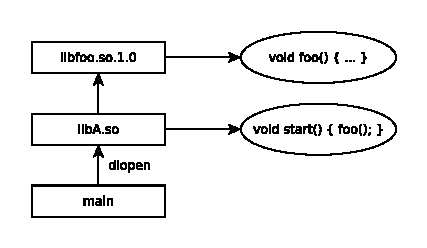
\includegraphics{figures/libdeps-ex1.pdf}
        \caption{Un exemple de dépendance de bibliothèques au sein d'un application simple fictive.
            La bibliothèque \textit{libA.so} est chargée dans l'application \texttt{main} via
            les appels aux procédures \textit{dlopen} et \textit{dlsym}. Les fonctionnalités utilisées
            dans l'exemple sont marquées dans des ellipses.
        }
        \label{fig:deps-ex1}
    \end{figure}
\end{center}

Dans la situation présentée dans la figure-\ref{fig:deps-ex1}, qu’elles sont les étapes incluses
dans l'exécution de ce programme qui invoque la fonctionnalité \texttt{start} de la
bibliothèque \textit{libA.so}. La fonctionnalité externe \texttt{start} est résolu de façon directe par
un appel à \verb|dlsym(libA, "start")|, qui commence la recherche de la procédure \texttt{start} dans
la bibliothèque spécifier dans \texttt{dlsym}. Le programme l'invoque une fois la procédure trouvée.
L'appel à une procédure non résolue (e.g.\ la procédure \texttt{foo} invoqué dans \texttt{start})
déclenche une procédure automatique de résolution des fonctionnalités. Cette procédure de résolution
commence sa recherche à partir de l'exécutable, puis itère la liste des dépendances directe. Si la
fonctionnalité n'est pas encore trouvé, la recherche continuera à partir de la bibliothèque passée à
\texttt{dlsym}.

% Stub

% TODO: exemple de résolution direct
Il est facile d'exploiter l'ordre de recherche du \textit{dynamic linker} pour
causer un masquage de fonctionnalité dans une application. Ce masquage est
utilisé dans certains contextes pour déboguer un programme, mais il peut aussi
nuire à l'exécution du programme. Il y au moins deux structures de programme
qui cause un masquage. L'application principale est construit comme une
bibliothèque dynamique exécutable et fournit une fonctionnalité qui porte le
même nom qu'une fonctionnalité exportée par une bibliothèque externe chargée
manuellement.  L'application principale est liée avec une bibliothèque qui
exporte une fonctionnalité qui porte le même nom que celle utilisée dans la
bibliothèque externe.

La figure-\ref{fig:deps-ex2} est un exemple de masquage qui utilise la seconde
méthode. La première méthode requiert des bibliothèques exécutables qui ne sont pas
disponibles sur toutes les plateformes. Sous Linux, il est possible de créer une
bibliothèque exécutable en passant le paramètre \texttt{-rdynamic} à \textit{gcc}
lors de la construction.

\begin{center}
    \begin{figure}[ht]
        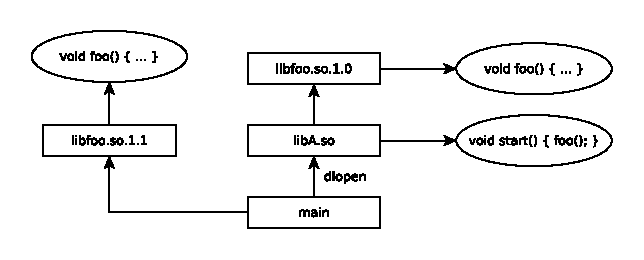
\includegraphics{figures/libdeps-ex2.pdf}
        \caption{Exemple de dépendance dans une application cause le masquage de la fonctionnalité \texttt{foo}
        de la bibliothèque \textit{libfoo.so.1.0} par la bibliothèque \textit{libfoo.so.1.1}}
        \label{fig:deps-ex2}
    \end{figure}
\end{center}
%% BEGIN
% D'autre langage compilé comme C/C++
% ne le permette pas directement, la liste des bibliothèques de code utilisé par un
% programme est déterminée lors de la création du fichier binaire, qui peut être
% soit un exécutable où une bibliothèque.
%% END


% TODO: pourquoi est-ce utile?
% XXX: structure pas final.
% - Les bibliothèques coexistent dans les application de tous les jours.
L'analyse des interactions entre des bibliothèques au sein d'un même programme permet de
mieux comprendre quelles sont les circonstances qui peuvent conduire à des comportements
non désirés, comme le masquage de fonctionnalité présent l'exemple de la figure-\ref{fig:deps-ex2}.
Cela permet aussi d'établir les conditions qui permettent d'éviter ces comportements non désirés.

\subsection{Coexistence entre les bibliothèques}

Les bibliothèques coexistent dans deux contextes principaux, de façon passive
dans un système fichier et de façon active durant l'exécution d'un programme.
Un système de fichier contient une arborescence hiérarchique de répertoires et
de fichiers avec une seule racine. Un fichier est l'entité dans un système de
fichier qui contient le code des bibliothèques.  Les répertoires sont les
entités qui permette de regrouper plusieurs fichiers de façon logique. La
racine correspond au sommet de la hiérarchie du système de fichier. La façon de
référer à un fichier dans un système de fichier est d'utiliser le
chemin absolu. Cela correspond à la liste des répertoires à parcourir de la
racine jusqu'au fichier. L'outil responsable d'organiser les bibliothèques sur
un système est le \textit{package manager}. Il a plusieurs objectifs
incluant l'installation de bibliothèque, la mise à jour des
bibliothèques installées, la désinstallation de bibliothèque et la résolution
des dépendances.

Un cas intéressant de coexistence entre bibliothèques est celui qui inclue
plusieurs versions d'une bibliothèque. Les problèmes peuvent être liés à
d'organisation sur le système de fichier et au masquage de fonctionnalité
durant l'exécution d'un processus.  Il y a aussi plusieurs utilités de
conserver plusieurs versions d'une bibliothèque, cela permet de supporter des
applications qui dépendent de bibliothèques antérieures.

Une autre application est de convertir un vieux format de fichier vers un format
plus récent. Dans le cas où il n'est pas possible de plusieurs versions d'une bibliothèque
il faut alors écrire un \textit{reader} pour lire le vieux format manuellement ensuite le
utilise fonctions de la version cible de bibliothèque pour générer le nouveau format du fichier.
Cette solution à comme problème que le \textit{reader} est beaucoup moins testé que la
vielle version de la bibliothèque. Cela demande aussi de réécrire qu'est-ce qui à déjà été fait.

\begin{figure}[ht]
  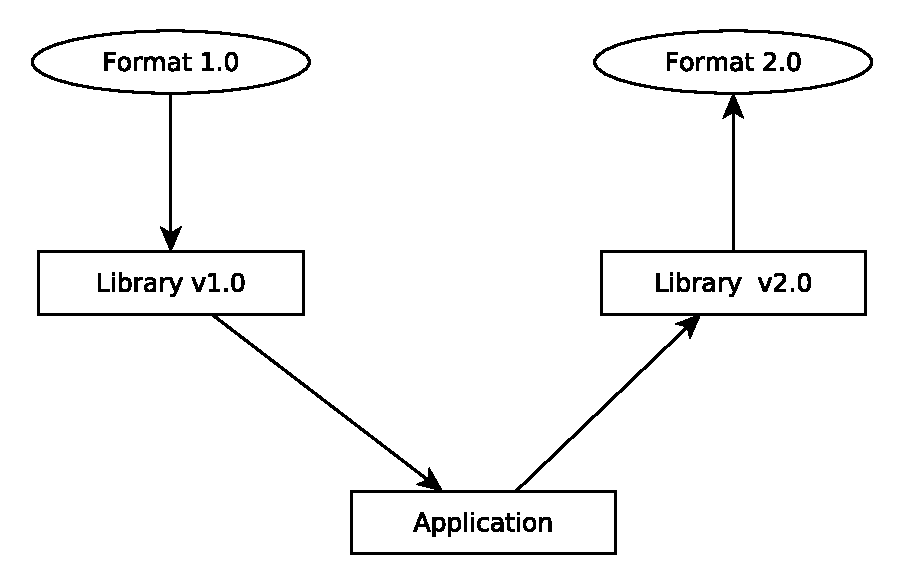
\includegraphics[width=30em]{figures/app_convert_v1_to_v2.pdf}
  \caption{Un exemple d'application de conversion entre deux version d'un format
  de fichier comme sqlite2 et sqlite3 exploitant la possibilité de charger plusieurs
  versions d'une bibliothèque.}
\end{figure}

% L'architecture de processus sur un système permet plusieurs propriétés. La
% robustesse, un processus failli les autres processus ne sont pas affectés. La
% sécurité et l'isolation, chaque processus possède leur mémoire qui n'est pas
% accessible par les autre processus et peuvent utilisé une version spécifique
% des bibliothèques. Il est possible de concevoir l'architecture de processus en
% utilisant des threads.  Un \textit{thread} décrit un courant d'exécution d'un
% programme. Un processus à au minimum un \textit{thread} qui correspond au
% courant d'exécution principal du programme. Les \textit{threads} sont utiles
% pour paralléliser l'exécution d'un processus. La création de \textit{threads}
% est beaucoup plus rapide que la création d'un processus, car elle ne nécessite
% pas l'appel au système d'exploitation.

% Ce modèle exploite la légèreté des \textit{threads} par rapport au processus et
% la possibilité de charger plusieurs version des bibliothèques qu'il a besoin au sein
% du système. Cela est similaire au modèle de processus utilisé par les
% système d'exploitation, sauf que l'ensemble est juste au sein d'un seul processus.
% Étant donnée que les \textit{threads} vivent tous au sein d'un même processus,
% il est donc facile de partagé des informations d'un \textit{thread} à un autre.
% Ce qui est plus difficile avec le modèle de processus, cela nécessite l'utilisation
% mécanisme comme la mémoire partagé.

%\todo{picture: Thread as Light process}

% TODO: exemple de chemin.

%et s'il c'est un cas qui peut
%contenir un coexistence néfaste.  Cela n'est possible que s'il est possible de
%distinguer les deux version de la bibliothèque et aussi répartir les appels à
%des fonctions de même nom à la bonne version de la bibliothèque.

\section{Conditions entre des versions des bibliothèques}
%
Des conditions suffisantes pour que deux bibliothèques puissent coexister
ensemble au sein d'un processus incluant deux versions de la même bibliothèque
sont l'absence d'état global ou local, et l'unicité des noms des fonctionnalités.
L'absence d'état garantit que chaque fonction de la bibliothèque retourne
toujours un résultat prévisible dans un contexte identique. Un cas extrême est
la pureté fonctionnelle, qui est avantageux dans un contexte
\textit{multi-threadé}, car il n'est pas possible d'avoir une condition de
course sur une donnée partagée. La pureté fonctionnelle garantit qu'il n'y a pas
d'assignation.  Le fait que chaque fonctionnalité est associée à un nom unique
cela inhibe la capacité d'une bibliothèque de masquer une fonctionnalité d'une
autre bibliothèque.


% Une condition de courses survient lorsque l'ordre des opérations d'un programme
% s'exécute dans un ordre que le programmeur n'a pas conçu. Par exemple, un
% application avec deux fils d'exécutions, un qui lit la valeur d'une variable
% globales l'autre qui l'écrit.  Deux scénarios sont possible, la lecture peut
% s'effectuer avant ou après la la modification de la variable globale selon
% l'ordonnancement de ces deux fils d'exécution.  Le résultat de la lecture est
% dépendant de l'ordonnancement de ces deux opérations.

Ces conditions sont suffisantes pour que deux bibliothèques coexistent sans
problème, mais elles ne sont pas nécessaires. Il existe des bibliothèques qui
ne respectent pas ces conditions, mais coexistent avec d'autres bibliothèques.
Pour tester la coexistence entre plusieurs bibliothèques, des expériences ont
été effectuées dans plusieurs systèmes de modules existants. Le but de
l'expérience est d'observer le bon fonctionnement des la bibliothèque au sein
de même processus.

Les expériences qui suivent permettent d'observer d'identifier les cas de cohabitation de bibliothèques
au sein d'une application qui cause des problèmes. Ils permettent aussi d'identifier les capacités d'un
langage à charger plusieurs versions d'une bibliothèque.

% XXX
%La capacité d'un langage d'interfacer avec d'autre langage via la FFI propage
%les limitations du langage cible.


\subsection{Bibliothèque C}
%
Les bibliothèques dans le langage C sont compilées dans un format natif pour la
plateforme courante (e.g. Window, MacOSX, Linux). Leur format diffère d'un
système d'exploitation à un autre, Window utilise le format \textit{dll}
(\textit{dynamic loading library}), MacOSX utilise le format \textit{dylib}
(\textit{Mach-O dynamic library}) et Linux utilise le format \textit{so}
(\textit{shared library}).

Les bibliothèques C consistent de symboles qui correspondent aux fonctions est
variables globales exportées. Une bibliothèque est généralement liée à un
programme C en lors de la création du programme. Les symboles non définis sont
résolus durant l'exécution du programme.

% TODO: complete
% - Bibliotheques avec collisions de nom de symboles
% - Masquage de fonctionnalité d'une des deux bibliothèque
Les collisions de symboles entre deux bibliothèques causent un masquage de
fonctionnalité d'une des deux bibliothèques. Un problème est de savoir si cela est
possible de charger deux bibliothèques avec des collisions de symboles et accéder aux
fonctionnalités distincts de ces bibliothèques.

Pour chargé deux versions d'une même bibliothèque en C, il faut utilisé un
moyen qui prend en compte des symboles communs.  La résolution des symboles ce
fait par un parcourt en largeur dans la liste des symboles des bibliothèques.
Le résultat est le premier objet qui correspond au nom de symbole recherché.
L'ordre des bibliothèques utilisé dans la résolution des symboles correspond à
l'ordre spécifié lors de la construction de l'exécutable.

%    \vspace{-10pt}
\begin{center}
\begin{figure}[ht]
\begin{lstlisting}[frame=single]
> gcc -lSDL -lSDL2 exemple.c -o exemple
> ldd ./exemple
libSDL.so => /usr/lib/libSDL.so
libSDL2.so => /usr/lib/libSDL2.so
\end{lstlisting}
\caption{Création d'un exécutable lié aux deux bibliothèques
SDL et SDL2 dans cette ordre.}
\label{fig:sdl_mask_sdl2}
\end{figure}
\end{center}

La figure \ref{fig:sdl_mask_sdl2} donne la procédure de création d'un
exécutable lié avec deux versions de SDL.  Les tests ont été effectués sur deux
versions de SDL, 1.2 et 2, ils peuvent utiliser des ressources communes comme
les évènements du clavier, la mémoire et le GPU en utilisant OpenGL pour faire
de l'affichage 2D ou 3D.  Plusieurs situations sont testées, chacune sans thread
et avec des threads:
%
\begin{enumerate}
    \item Une utilisation de SDL minimaliste qui n'écoute pas les évènements utilisateurs.
    \item Une utilisation de SDL avec une boucle d'évènements de base.
    \item Une utilisation de SDL avec une utilisation d'un contexte OpenGL.
\end{enumerate}

%% SDL1.2 appel ces propres fonctions et SDL2 appel ces propres fonctions.
Puisque SDL1.2 et SDL2 ont des collisions de symboles (i.e.\ \verb+SDL_Init+,
\verb+SDL_FillRect+, \verb+SDL_BlitSurface+, \dots), l'une des premières
observations à effectuer est la bonne répartition des appels de fonctions des
deux bibliothèques dans le contexte d'une même application. Le problème à
identifier est un appel invalide à une procédure de SDL2 qui était destiné à
SDL1.2. Le facteur qui influence laquelle des deux bibliothèques va masquer
l'autre est l'ordre dans laquelle ils sont liés au programme à la création,
qui est montrée à la figure-\ref{fig:sdl_mask_sdl2}.

Le masquage est une problématique qui peut mener à une défaillance du
programme, car cela peut provoquer la transmission d'une structure incompatible
de la première bibliothèque à la deuxième. Dans le cas de SDL, la structure
\verb+SDL_Surface+ à une disposition différente des champs, donc incompatible.
Le premier champ qui décale l'alignement de ces deux structures est le
\textit{pitch}, qui dans SDL1.2 est déclaré en Uint16 alors qu'en SDL2 il est
un int qui sont des types de taille différente. Donc, l'accès au prochain champ
\texttt{pixels} est différent entre SDL1.2 et SDL2, ce qui peut causer un accès
non désiré en mémoire si une structure de SDL1.2 est accédé comme une structure
de SDL2.

\begin{figure}[h]
  \centering
\begin{tabular}{p{18em}p{18em}}
\begin{lstlisting}[frame=single,numbers=left]
typedef struct SDL_Surface {
    Uint32 flags;
    SDL_PixelFormat *format;
    int w, h;
    Uint16 pitch;
    // Different offset here
    void *pixels;
    ...
} SDL_Surface;
\end{lstlisting}&
\begin{lstlisting}[frame=single,numbers=right]
typedef struct SDL_Surface {
    Uint32 flags;
    SDL_PixelFormat *format;
    int w, h;
    int pitch;
    // Different offset here
    void *pixels;
    ...
} SDL_Surface;
\end{lstlisting}\\
\end{tabular}
  \caption{C'est la comparaison entre la structure \textbf{SDL\_Surface} de SDL1.2 et SDL2 respectivement.}
  \label{fig:sdl_surface}
\end{figure}

%% Instable: gcc -lSDL -lSDL2 ...
%Puisque les programmeurs cherchent une certaine stabilité dans leurs bibliothèques, ils ont
%tendance à éviter les dépendances avec des bibliothèques qui ont des collisions de fonctionnalités.

La cohabitation entre deux bibliothèques conflictuelles au sein d'une application n'est pas possible
en lien l'application au bibliothèques durant sa construction~\ref{fig:sdl_mask_sdl2}.
Il est peu probable d'avoir une cohabitation entre deux bibliothèques avec des noms de fonctionnalités
similaires au sein.
% XXX: continue here

La façon d'avoir plusieurs bibliothèques conflictuelles au sein d'un programme 

Le cas qui pourrait permettre plusieurs bibliothèques avec des collisions de symboles
au sein d'une même est avec l'API du \textit{dynamic linker}. Un test simple permet
de démontrer la capacité de répartir les appels d'une fonction identifiés par le même nom
dans différentes bibliothèques.

La structure générale des tests est organisée comme suit. Deux bibliothèques implémentant
une interaction valide avec l'une des versions de la bibliothèque (e.g. SDL1.2, SDL2).
Une application qui unit ces deux bibliothèques en utilisant l'API du
\textit{dynamic linker} pour exécuter ces deux bibliothèques séquentiellement ou
parallèlement.

%% TODO: expliquer la structure des programmes.

Dans le test minimaliste sans gestion d'évènements, l'exécution des bibliothèque
fonctionne dans les deux cas, séquentiellement et en parallèle. La raison qui
explique ce bon fonctionnement est la répartition des appels au fonctions
des deux bibliothèques et le fait qu'il n'utilise pas de structure commune,
qui pourrait causer des conditions de course dans le test en parallèle.

\begin{center}
  \begin{figure}[ht]
\begin{lstlisting}[language=C,frame=single]
#include <SDL/SDL.h>

int main(int argc, char **argv) {
  SDL_Init(SDL_INIT_VIDEO);
  SDL_WM_SetCaption("sdl1_2", NULL);
  SDL_Surface *win =
    SDL_SetVideoMode(200, 200, 24, SDL_HWSURFACE);

  Uint32 color = SDL_MapRGB(win->format, 255, 0, 0);

  SDL_FillRect(win, NULL, color);
  SDL_Flip(win);
  SDL_Delay(1000);

  SDL_FreeSurface(win);
  SDL_Quit();
  return 0;
}
\end{lstlisting}
    \caption{Programme qui utilise la bibliothèque SDL1.2 sans la gestion des évènements
    Cette application génère une fenêtre rouge qui se ferme après 1 seconde de délais.}
  \end{figure}
\end{center}

%TODO: wrap these into frame
\begin{center}
  \begin{figure}[ht]
\begin{lstlisting}[language=C,frame=single]
#include <SDL2/SDL.h>

int main(int argc, char **argv) {
  SDL_Init(SDL_INIT_VIDEO);
  SDL_Window *win = SDL_CreateWindow("title",
      SDL_WINDOWPOS_CENTERED, SDL_WINDOWPOS_CENTERED,
      200, 200, SDL_WINDOW_SHOWN);
  SDL_Surface *screen = SDL_GetWindowSurface(win);

  Uint32 color = SDL_MapRGB(screen->format, 0, 255, 0);
  SDL_FillRect(screen, NULL, color);
  SDL_UpdateWindowSurface(win);
  SDL_Delay(1000);
  SDL_DestroyWindow(win);
  SDL_Quit();
  return 0;
}
\end{lstlisting}
    \caption{Programme qui utilise la bibliothèque SDL2 sans la gestion des évènements.
    Cette application génère fenêtre verte qui se ferme aussi après 1 seconde de délais.}
  \end{figure}
\end{center}

Dans le test incluant des évènements, l'hypothèse supposait que les évènements du clavier
aurait causé des problèmes de conditions de course en parallèle. Le test a aussi fonctionné
séquentiellement et en parallèle, malgré la dépendance commune du clavier.

Le test qui incluait OpenGL, n'aurait pas dû fonctionner par hypothèse. Les deux versions
de SDL référaient à une unique version de OpenGL. Le résultat a été surprenant, car le test
séquentiel et parallèle à fonctionné. Ce qui amène à conclure qu'il existe des cas
de coexistence entre des bibliothèques avec des collisions de symbole qui fonctionne
sans causer des problèmes d'exécution.



%%% Possible de compile le programme principale en un exécutable et en bibliothèque.
%Les deux programmes sont compilés en bibliothèques et en exécutables.
%Le fonctionnement de chaque programme est testé de façon séparé.
%Le programme principale, qui charge le main des deux autres programmes en utilisant
%l'API du \textit{dynamic loader}, est compilé en mode séquentiel et en mode parallèle.
%La version séquentielle permet d'observer la coexistance entre les deux bibliothèques,
%celle parallèle est utilisé pour évaluer les conditions de course sur des ressources
%communes.
%
%%% TODO: schema.
%\begin{center}
%  \begin{figure}[ht]
%\begin{lstlisting}[language=C,frame=single]
%  ...
%  void *hndl1 = dlopen(prog1, RTLD_NOW);
%  void *hndl2 = dlopen(prog2, RTLD_NOW);
%
%  int(*main1)(int,char**) = dlsym(hndl1, "main");
%  int(*main2)(int,char**) = dlsym(hndl2, "main");
%
%  main1(argc, argv);
%  main2(argc, argv);
%  ...
%\end{lstlisting}
%  \caption{Le chargement et exécution séquentiel de la fonction main des programmes
%  \textbf{prog1} et \textbf{prog2} via l'API du \textit{dynamic loader}.}
%  \end{figure}
%\end{center}
%% \begin{center}
%%   \begin{figure}[ht]
%% \begin{lstlisting}[language=C,frame=single]
%% struct MainCallback {
%%   int argc;
%%   char **argv;
%%   int (*main)(int,char**);
%% };
%%
%% void *run(void* args) {
%%   struct MainCallback* callback = (MainCallback*)args;
%%   callback->main(callback->argc, callback->argv);
%%   return NULL;
%% }
%% \end{lstlisting}
%%   \caption{Callback utilisé pour exécuté le main de la bibliothèque chargé par
%%   \textbf{dlsym} en parallèle avec pthread.}
%%   \end{figure}
%% \end{center}
%
%\begin{center}
%  \begin{figure}[ht]
%\begin{lstlisting}[language=C,frame=single]
%  ...
%  struct MainCallback callback = {
%    .argc = argc,
%    .argv = argv,
%    .main = main1
%  };
%
%  pthread_t th1;
%  pthread_create(&th1, NULL, run, &callback);
%  main2(argc, argv);
%  pthread_join(th1, NULL);
%  ...
%\end{lstlisting}
%    \caption{Exécution du code des deux programme en parallèle avec l'utilisation de pthread.
%    Contrairement à la figure précédente, la fonction main de \textbf{prog1} exécuté dans un
%    threads.}
%  \end{figure}
%\end{center}
%
%
%Tout d'abord, la compatibilité entre SDL1.2 et SDL2 à été testé par un code sans
%la gestion des évènements, pour vérifier si les fonctions respective de chaque
%bibliothèque étaient à appellé correctement.
%% coexistance sans interraction directe.
%#ifdef THREADED

% SDL1.2/SDL2/OpenGL
% - Hypothèse
%   - Non-threaded without OpenGL
%   - Non-threaded with OpenGL
%   - Threaded without OpenGL
%   - Threaded with OpenGL
% - Démarche
% - Résultat
% - Petite Conclusion

% OpenSSL+RSA/OpenSSL+Socket
% - Hypothèse
% - Démarche
% - Résultat
% - Petite Conclusion

\clearpage
\subsection{Bibliothèque Scheme avec FFI}
La compatibilité entre versions a été testée sur la partie cryptographique
RSA de OpenSSL, SDL et un générateur aléatoire qui possède un état global.
Pour observer le comportement de bibliothèque Scheme liant des fonctionnalités
implémenté dans un autre langage, dans ces exemple C. Ces tests montrent le problème
de masquage décrit précédemment dans des bibliothèques réelle.
Pour tester les bibliothèques natives en Scheme, il a fallut écrire des
un code spécial pour lier les types et les fonction au monde Scheme. Ces

Par hypothèse la partie cryptographique des deux versions de OpenSSL peuvent
coexister. Chacune des fonctions cryptographique de OpenSSL1.0 et OpenSSL1.1
exécute du code disjoint qui n'interfère pas avec une zone mémoire commune.
Cela implique qu'un appelle à une fonction de OpenSSL1.0 n'affectera pas les
résultats des appelles futures de OpenSSL1.1. Les fonctions nécessaires
pour tester la partie cryptographique RSA sont:
\begin{itemize}
    \item \lstinline{PEM_read_bio_RSA_PUBKEY} et \lstinline{PEM_read_bio_RSAPrivateKey}:
        Ce sont les fonctions OpenSSL qui permettent de lire la clef publique et la clef privée.
    \item \lstinline{RSA_public_encrypt}:
        La fonction de cryptage qui crypte un  message en utilisant une clef publique.
    \item \lstinline{RSA_private_decrypt}:
        La fonction qui permet de décrypter un message en utilisant la clef privée.
    \item \lstinline{RSA_free}:
        La fonction qui libère la mémoire allouée pour les clefs publiques et privées.
        Cette fonction n'est pas nécessaire pour les tests, mais utile pour une bonne
        gestion mémoire.
\end{itemize}
La structure de donnée utilisée par les fonctions d'OpenSSL pour la cryptographie RSA
est un pointeur vers un enregistrement RSA. La liaison avec le type C est effectuée avec
la forme spéciale \lstinline{c-define-type}.

Le test consiste à crypter un message en utilisant une clé publique, décrypter le
cryptogramme avec la clé privée et comparer le message original avec le message décrypter
pour les deux versions de OpenSSL chargé dans le même processus. Pour vérifier la bonne
invocation des fonctions de OpenSSL1.0 et OpenSSL1.1 respectifs, le débogueur \textbf{gdb}
a été utilisé. Les bibliothèques d'OpenSSL consistent en deux fichiers \url{libssl.so} et \url{libcrypto.so}.
En déboguant la répartition des appels avec \textit{gdb}, il y a eu l'observation que
la bibliothèque \url{libcrypto.so} de OpenSSL1.1 masquait la version de OpenSSL1.0 s'il
n'est pas spécifié explicitement lors de la création de la bibliothèque Scheme \textit{rsa.scm}
comme à la figure-\ref{fig:scm_masq1}. Les raisons sont liées à plusieurs facteurs qui étaient présents
durant l'expérience. L'ordre de recherche des symboles qui inclue les symboles des bibliothèques liés à
l'exécutable qui sont prioritaire qui contenait \url{libssl.so} et \url{libcrypto.so} de OpenSSL1.1.
Dans ce cas, il était possible de résoudre ce problème en ajoutant une
dépendance directe à \textit{libcrypto} lors de la construction des bibliothèques Scheme \verb+RSA+
comme montré dans la figure-\ref{fig:scm_masq_fix1}.

\begin{center}
\begin{figure}[ht]
\begin{lstlisting}[frame=single]
gsc-script -o rsa-1-0-0.o1 \
  -cc-options '-I /usr/include/openssl-1.0' \
  -ld-options '-L /usr/lib/openssl-1.0 -lssl' \
  -prelude '(define-cond-expand-feature|openssl-v10|)' rsa.scm

gsc-script -o rsa-1-1-0.o1 \
  -ld-options "-lssl" rsa.scm
\end{lstlisting}
\caption{Création des bibliothèques \textit{rsa.scm} pour OpenSSL1.0 et OpenSSL1.1
sans la spécification de \textit{libcrypto.so}}
\label{fig:scm_masq1}
\end{figure}
\end{center}

\begin{center}
\begin{figure}[ht]
\begin{lstlisting}[frame=single]
gsc-script -o rsa-1-0-0.o1 \
  -cc-options '-I /usr/include/openssl-1.0' \
  -ld-options '-L /usr/lib/openssl-1.0 -lssl -lcrypto' \
  -prelude '(define-cond-expand-feature|openssl-v10|)' rsa.scm

gsc-script -o rsa-1-1-0.o1 \
  -ld-options "-lssl -lcrypto" rsa.scm
\end{lstlisting}
\caption{Création des bibliothèques \textit{rsa.scm} pour OpenSSL1.0 et OpenSSL1.1
avec la spécification de \textit{libcrypto.so}}
\label{fig:scm_masq_fix1}
\end{figure}
\end{center}

\begin{center}
\begin{figure}[ht]
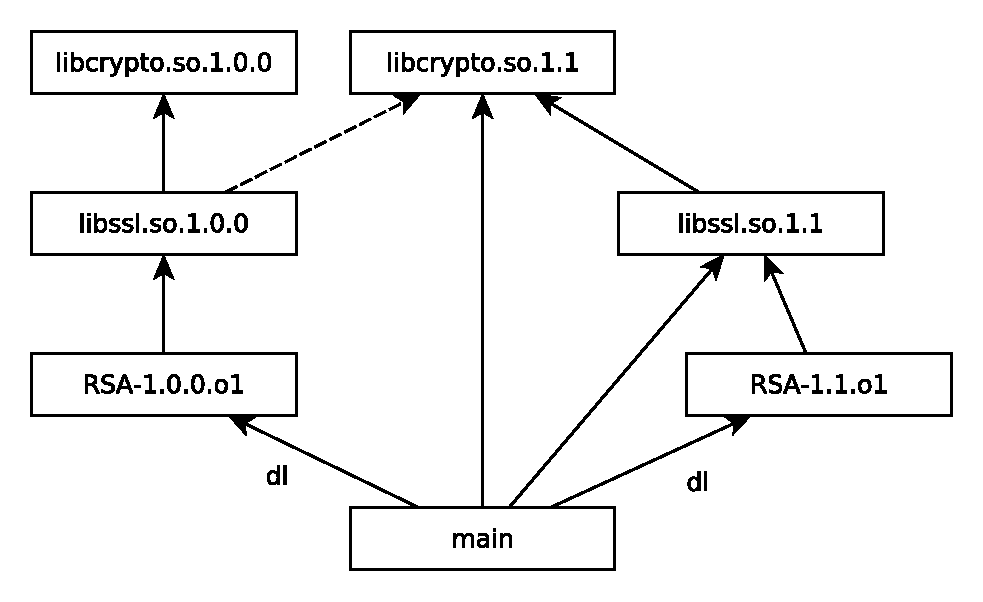
\includegraphics{figures/libssl_masking.pdf}
\caption{Schéma des dépendances entre les bibliothèques au sein d'un processus.
Les dépendances qui ont été lié dynamiquement lors la création de l'application sont représentés par une flèche avec
trait plein sans annotation. Ceux qui représente les chargement de bibliothèque dynamique via \texttt{dlopen} ont
l'annotation \textit{dl}. La flèche en pointillé indique un masquage des symboles de la bibliothèque
source par celle pointée.}
\label{fig:scm_masq_schema}
\end{figure}
\end{center}

TODO: rng générator

%\begin{lstlisting}[frame=single]
%(c-define-type RSA* (pointer "RSA"))
%\end{lstlisting}


%Heureuse Gambit Scheme possède un interface pour lié
%une fonction C au monde Scheme.

%Une bibliothèque liant les fonctions principales de SDL au monde Scheme.


%\TODO{Fill}
% SDL / SDL2
% - Hypothèse
% - Démarche
% - Résultat
% - Petite Conclusion

% OpenSSL+RSA
% - Hypothèse
% - Démarche
% - Résultat
% - Petite Conclusion

% RNG-splitmx64/RNG-xoroshiro128+
% - Hypothèse
% - Démarche
% - Résultat
% - Petite Conclusion


\subsection{Bibliothèque JavaScript (NodeJS)}
%\TODO{Fill}
% Démarche général
% express / sqlite3
% - Hypothèse * 2
% - Démarche/Expérimentation
% - Résultat
% - Petite Conclusion

Pour effectuer des tests sur la coexistence de différente version d'une bibliothèque
JavaScript dans NodeJS, il faut tout d'abord permettre l'importation de plusieurs
versions d'une même bibliothèque. Dans NodeJS, l'importation de modules s'effectue
avec la fonction \verb|require(module-name)|. Puisque l'information de version
de la bibliothèque n'est pas fournie en paramètre à la fonction, il faut donc
utilisé une autre méthode de forcer plusieurs versions des bibliothèques.
La configuration d'un module dans NodeJS utilise le format JSON pour spécifier
le nom, la version, les dépendances \dots.

Les dépendances sont conservées sous la forme d'un arbre, chaque module à ses dépendances directes
qui ont aussi des dépendances indirectes.  Lors de l'écriture d'un module JavaScript, il est possible
de spécifier la version de chaque dépendance dans le fichier \textit{package.json}.
\begin{verbatim}
{
  ...
  "dependencies": {
    "express": "4.16.3"
  },
  ...
}
\end{verbatim}
En utilisant cette fonctionnalité du système de module de NodeJS, deux bibliothèques \textit{wrapper}
sont écrites pour interfacer les deux versions de express. Puisque l'API public d'express n'a pas changé entre
les versions 3.21.1 et 4.16.3, il est possible de recycler le code de la bibliothèque qui encapsule une
version d'express (figure-\ref{fig:express}).
\begin{center}
\begin{figure}[ht]
    % FIXME: language=Javascript
    \begin{lstlisting}[language=C,frame=single]
const express = require('express');

function start() {
  const app = express();
  const port = Math.floor(Math.random() * 64535 + 1000);

  app.get('/', (req, res) => {
    res.send('Hello world!\n');
  });

  app.listen(port, 'localhost', () => {
    console.log('Listen on port ' + port);
  });
}
exports.start = start;
\end{lstlisting}
\end{figure}
\label{fig:express}
\end{center}
Le programme principal ne fait qu'importer les deux encapsulations de bibliothèque
et invoque la fonction \textit{start}.

Le résultat attendu dans cette expérience est que ces deux versions de la bibliothèque
express coexistent sans problème, sauf dans le cas où le port tcp utilisé par les deux
versions est le même. Dans ce cas, c'est la bibliothèque dont la fonction
\textit{start} a été invoqué en premier qui va monopoliser le tcp port. Dans ce cas
la ressource qui inhibe la coexistence de ces modules au sein d'un même processus
est liée au \textit{socket}.

\subsection{Variables globales communs}

Puisque qu'il n'existe qu'une seule instance de chaque bibliothèque en mémoire, cela implique
que les variables globales d'une bibliothèque.

Définissons 3 bibliothèques B, C et D telle que D a une variable globale nommée \textit{value}.
B et C ont chacun une dépendance directe vers D, et exportent une référence de la variable
globale \textit{value} de D.

Le programme principal A commence par charger B et C. Ensuite lit la valeur de \textit{B.D.value}
puis modifie \textit{C.D.value} et relit \textit{B.D.value}. Le test réussi si la valeur de
\textit{B.D.value} reste inchangé par la modification de \textit{C.D.value}. Cela implique que
les références vers la bibliothèque D est différentes de via B et via C.

Dans NodeJS, un module peut être installé via un dossier, une archive tarball, un dépôt de code source git ou
directement via Npmjs. Puisqu’un module publié dans Npmjs ne peut pas être retiré facilement étant donné
la politique liée au module (\url{https://docs.npmjs.com/cli/unpublish}).
%L'expérience va utilisé un serveur git qui est auto-hébergé.

% TODO: shift chapter number.

\chapter{Implémentation des modules}

Le format des modules nécessite plusieurs composantes.
Chaque module doit avoir sont propre espace de nom
disjoint des autres modules. Un liste d'importation
qui indique les dépendances entre les modules et permet
l'interaction entre les modules. Certaines formes spéciales
ont été ajouté dans pour pouvoir exprimer les relation entre
les modules.

\section{Formes spéciale}

Les espaces de nom sont gérer avec une forme spécial propre à Gambit. Cet forme
se nomme \lstcode{##namespace}.  La seul restriction sur les espaces de nom
dans Gambit est qu'ils doit se terminer par le caractère \lstcode{#}.
La forme \lstcode{##namespace} permet de préfixer et renommé des identifiants
dans un contexte.

Cela permet de créer un espace distinct pour chaque module. Cela permet
d'éviter les conflits de nom entre les modules tant que les espaces de nom sont
différents. Chaque module commence par déclarer son espace de nom suivit des
définitions des procédures du module. Une déclaration d'espace de nom à la forme
suivante \lstcode{(##namespace ("<name>#"))}. La partie \lstcode{<name>} de la
forme \lstcode{##namespace} doit être un chaine d'au moins un caractères.

\begin{center}
  \begin{tabular}{|l|}
\hline
\begin{mplisting}{0.6}
;; example.scm
(##namespace ("example#" hello))
(define (hello)
  (display "Hello, world!\n"))
(hello)
\end{mplisting}\\\hline
  \end{tabular}
\end{center}
L'exemple ci-dessus est un exemple d'utilisation de la forme \lstcode{##namespace}











Gambit offre un mécanisme pour aider a minimiser les conflits de nom. Ce
mécanisme permet d'associer un identifiant à un autre avec la forme spécial
\lstcode{##namespace}.  L'appel à \lstcode{(##namespace ("foo#" A B))} indique
qu'une référence futur à \lstcode{A} devient une référence à
\lstcode{foo#A} et l'un à \lstcode{B} devient une à \lstcode{foo#B}. Le espace
de nom dans lequel \lstcode{A} et \lstcode{B} est \lstcode{foo#}.

\begin{center}
  \begin{figure}[h]
  \begin{tabular}{|l|}
\hline
\begin{mplisting}{0.5}
;; math#.scm
(##namespace ("math#" fact fib))
\end{mplisting} \\\hline
\begin{mplisting}{0.6}
;; math.scm
(##namespace ("math#" fact fib))
(define (fib n)
  (if (< n 2)
    n
    (+ (fib (- n 1)) (fib (- n 2)))))
(define (fact n)
  (if (< n 2)
    1
    (* n (fact (- n 1)))))
\end{mplisting}\\\hline
  \end{tabular}
  \caption{Écriture d'un petit module mathématique qui implémente les fonctions \lstcode{fact}
    et \lstcode{fib}. Ce module est séparé en 2 fichiers, \texttt{math\#.scm} est un fichier
    contenant les déclarations de l'espace de noms et des définitions de macros que le module
    exporte.}
  \label{fig:math_module1}
\end{figure}
\end{center}
% XXX: END implementation

%\begin{center}
%  \begin{figure}[h]
%  \begin{tabular}{|l|l|}
%\hline
%\begin{mplisting}{0.5}
%;; Library
%(library (math)
%  (export fact)
%  (import (rnrs base))
%  (define (fact n)
%    (if (< n 2)
%      1
%      (* n (fact (- n 1))))))
%\end{mplisting} &
%\begin{mplisting}{0.5}
%;; Main program
%(import
%  (rnrs base)
%  (rnrs io simple)
%  (math))
%
%(display (fact 5))
%(newline)
%\end{mplisting}\\\hline
%  \end{tabular}
%\caption{À gauche, il y a un exemple d'une bibliothèque mathématique dans le format R6RS qui implémente
%la fonction factoriel. À droite, un exemple d'importation de la bibliothèques qui utilise la forme
%spéciale \texttt{import}.}
%\end{figure}
%\end{center}

\section{Implémentation des modules systèmes}

\section{Implémentation des modules R7RS}
% XXX: Implémentation


\chapter{Modèle de chargement}
\label{ch:loading-model}

Un système est composé d'un ensemble d'éléments (modules) qui interagissent
entre eux.  Une bibliothèque fait office de module au sein d'un système simple
ou complexe.

\section{Chargement des bibliothèques}

%La collection des modules s'effectue au sein d'un

% TODO: voir chargé
Le chargement d'une bibliothèque Scheme (ou module) est séparé en plusieurs niveaux.
% TODO: now
Les bibliothèques sont soit lu du disque vers la mémoire durant l'exécution
ou déjà dans la mémoire du processus. Durant la compilation les modules sont
collecté pour construire un exécutable. Le chargement
d'une bibliothèque inclut une phase de recherche sur le système de fichier pour valider
l'existence de la bibliothèque et des fonctionnalités demandés. L'emplacement des
bibliothèques sur le système de fichier est lié par défaut aux chemin spécifié par
le \lstinline{##module-search-order} a comme défaut \lstinline{~~lib} et \lstinline{~~userlib}.


La procédure exacte de chargement des bibliothèques par \verb|import|
n'est pas spécifier par le standard R7RS. Le standard spécifie seulement la syntaxe
à utilisé et le de comportement principal qui est
requis. L'importation d'une bibliothèque doit chargé la bibliothèque
et rendre c'est fonctionnalité disponible dans le contexte
l'importation a eu lieu qui peut soit ovenir d'un programme principale
ou d'une bibliothèque.

Le chargement d'une bibliothèque peut-être effectuée à l'exécution par
l'utilisation de \texttt{eval} (par \texttt{load}) pour les fichiers source et
\texttt{load-objcet-file} pour les bibliothèques compilées. Cette recherche
peut aussi avoir lieu durant l'édition des lien en utilisant les méta-infos
contenus dans les \textbf{.c} qui sont chacun compilé par le compilateur C
en \textbf{.o} et lié par le \textit{linker}.

\section{Modèle dynamique}
Dans ce modèle les bibliothèques sont lié au programme durant l'exécution. Cela
nécessite que les bibliothèques soit organisé sur le système de fichier d'une façon
distingable. Chaque module doit posséder un nom unique qui permet d'y référer.
Ce nom unique va être utilisé lors de la collection des dépendances.


%Les bibliothèques
%sont soit en code source ou compilé nativement avec l'extension (\textit{.oN})
%où le N correspond à la version du binaire qui commence à 1.


La recherche des bibliothèques est effectué dans un ordre spécifique
indépendant de la spécification.  L'algorithme de recherche les bibliothèques
prend entré le nom de la bibliothèque et retourne le chemin absolu
correspondant à sont emplacement dans l'arborescence du système de fichier. Les
bibliothèques sont situées dans différents répertoires l'origine du programme,
le répertoire des bibliothèques système (\lstinline{~~lib}) et le
répertoire de bibliothèque utilisateur (\lstinline{~~userlib}).

% \begin{itemize}
%   %% XXX: directory where the executable is located (usefull for devel no need to install the module). collecté
%   \item \verb|origin/dummy.sld|
%   \item \verb|origin/dummy/dummy.sld|
%   \item \verb|~~userlib/dummy.sld|
%   \item \verb|~~userlib/dummy/dummy.sld|
%   \item \verb|~~lib/dummy.sld|
%   \item \verb|~~lib/dummy/dummy.sld|
% \end{itemize}

Chaque module possède trois niveau d'initialisation dans le système numéroté de
0 à 2. Le niveau 0 indique que le module n'a pas été initialisé. Ces les niveau
des module qui ont juste été collecté par le système. Le niveau 1 indique que
le descripteur du module à été récupéré. L'étape 2 est utilisé pour indiquer
les module chargé.

Soit un système avec les dépendance suivante:
\begin{figure}[ht]
  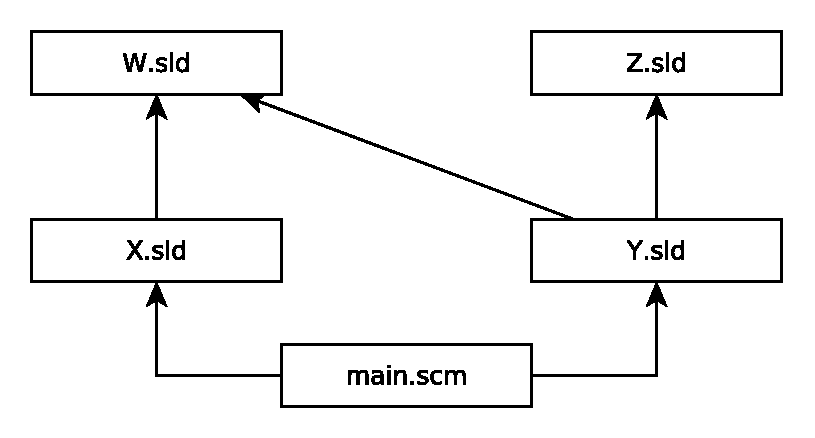
\includegraphics{figures/system-example}
  \caption{Un exemple d'un système fictif composé de différents modules.
  Le module principale se nomme utilise l'extension \textbf{.scm}
  et les bibliothèques porte l'extension \textbf{.sld}}
\end{figure} % TODO: use yed for that graph


Le démarrage du module principal Main.scm déclenche la collection des modules X
et Y, qui récursivement déclenche la collection de W et Z. L'algorithme de
collection des modules ignore les module qui apparaisse plusieurs fois au sein
du graphe.

Une fois la collection de tous ces modules est complété le descripteur de
module est récupéré par un appels à \verb|dlopen| et \verb|dlsym| dans le cas
compilé.


\section{Module hébergé}

Un module qui est hébergé est un module qui dont son contenu
se retrouve sur un domain comme \url{github.com}.\\
\begin{center}
  \lstset{caption={Grammaire BNF représentant un hostname selon un sous
  ensemble du RFC-2396.},captionpos=b,frame=single}
  \begin{mplisting}{0.9}
hostname      = +( domainlabel "." ) toplabel
domainlabel   = alphanum | alphanum *( alphanum | "-" ) alphanum
toplabel      = alpha | alpha *( alphanum | "-" ) alphanum
alphanum      = alpha | digit
alpha         = [a-zA-Z]
digit         = [0-9]
\end{mplisting}
  \label{lst:hostname->grammar}
\end{center}

La différence avec la spécification du hostname dans le RFC-2396
est que le hostname ne peut pas finir par un point et doit contenir
au moins un \verb|domainlabel|. C'est pour permettre de distingué
un module local et un module hébergé.

\subsection{Module \texttt{\_git}}

Ce module offre un interface pour utiliser interagir avec les des dépôts git.
Il permet de cloner un dépôts qui est hébergé sur \url{github.com}. Un clone du
dépôts est simplement un copie qui contient les informations suffisantes pour
passer d'une version d'un module à un autre. L'opération qui permet de changer
de version est \emph{checkout}.


%-------------------------------------------------------------------------------
%
%Modèle "link dynamique" :
%  recherche des libs au run time, utilisation de eval (par load) et
%  load-object-file
%
%  % gsi main.scm      ou      % gsc main.scm ; gsi main.o1
%
%    origin/main.scm    : (import X Y)
%          /X/X.sld     : (import)
%
% ~~userlib/Y/Y.sld     : (import Z)
%
%     ~~lib/Z/Z.sld     : (import)
%          /Z.o1
%
%-------------------------------------------------------------------------------
%
%Modèle "link statique" :
%  recherche des libs au link time en utilisant les méta-infos
%  dans les .c (demand-lib et supply-lib), chaque .c compilé en
%  un .o séparément et les .o linkés par le compilateur C
%
%  % gsc -obj -keep-c X.sld      ;; créer .c et .o
%  % gsc -obj -keep-c Y.sld      ;; créer .c et .o
%  % gsc -obj -keep-c Z.sld      ;; créer .c et .o
%  % gsc -obj -keep-c main.scm   ;; créer .c et .o
%  % gsc -exe main.c             ;; combine les .o pour créer main.exe
%
%    origin/main.scm    : (import X Y)
%          /main.c      : (demand-lib X Y)
%          /main.o
%          /X/X.sld     : (import)
%            /X.c       : (demand-lib) (supply-lib X)
%            /X.o
%
% ~~userlib/Y/Y.sld     : (import Z)
%          /Y/Y.c       : (demand-lib Z) (supply-lib Y)
%          /Y/Y.o
%
%     ~~lib/Z/Z.sld     : (import)
%          /Z/Z.c       : (demand-lib) (supply-lib Z)
%          /Z/Z.o
%
%-------------------------------------------------------------------------------
%
%Modèle "whole-program" :
%  recherche des libs au compile time en utilisant les imports
%  dans les fichiers sources, les AST de toutes les libs fusionnées
%  en un seul AST compilé par gsc (donc un seul .c généré et compilé
%  par le compilateur C pour créer main.exe)
%
%  % gsc -exe -whole-program main.scm
%
%    origin/main.scm    : (import X Y)
%          /X/X.sld     : (import)
%
% ~~userlib/Y/Y.sld     : (import Z)
%
%     ~~lib/Z/Z.sld     : (import)
%
%-------------------------------------------------------------------------------
% correction d’une petite coquille…
% /Y.c       : (demand-lib Z) (supply-lib Y)
% /Y.o
%
% ~~lib/Z/Z.sld     : (import)
% /Z.c       : (demand-lib) (supply-lib Z)
% ...


% (check-sld "/tmp/scheme/base/base.sld" "/tmp/scheme/base")
% (check-sld "/tmp/scheme/base.sld" "/tmp/scheme")
% (check-sld
%  "/home/frederic/Documents/MasterResearch/gambit9/lib/cocolappin/scheme/base/base.sld"
%  "/home/frederic/Documents/MasterResearch/gambit9/lib/cocolappin/scheme/base")
% (check-sld
%  "/home/frederic/Documents/MasterResearch/gambit9/lib/cocolappin/scheme/base.sld"
%  "/home/frederic/Documents/MasterResearch/gambit9/lib/cocolappin/scheme")
% (check-sld
%  "/home/frederic/Documents/MasterResearch/g9/lib/scheme/base/base.sld"
%  "/home/frederic/Documents/MasterResearch/g9/lib/scheme/base")
% object-file-path: /home/frederic/Documents/MasterResearch/g9/lib/scheme/base/.gambit_409003@C/base.o1
% ("/home/frederic/Documents/MasterResearch/g9/lib/scheme/base/base.sld"
%  .
%  #<input-port #2 "/home/frederic/Documents/MasterResearch/g9/lib/scheme/base/base.sld">)


\chapter{Gestion des modules}
\label{ch:module_management}

% TODO: too much detail in intro
%       il ne faut pas faire un sommaire du carteau du chapitre, mais motiver
%       l'existance de ce chapitre
%       et mentionner ce dont tu va parler et pourquoi (le lien avec ce travail)

Ce chapitre décrit l'organisation des modules sur le système de fichier pour
permettre plusieurs versions d'un module. Notre approche est d'associer à
chaque version d'un module un répertoire différent. Cela permet de stocker les
différentes versions d'un module dans le système de fichier.  Nous avons
comparé les différentes façons d'organiser les modules dans plusieurs langages
comme Python, JavaScript, Go, OCaml. Il est important que l'installation d'un
module n'altère pas le bon fonctionnement des autres modules.  Le modèle de gestion des
modules choisi garantit que les dépendances d'un module sont fixes.

\section{Sommaire}
% Installation, Désinstallation, Mise à jour, Compilation/Exécution
La gestion des modules inclut généralement l'installation, la mise à jour et
la désinstallation. L'organisation des modules est un élément important
dans la gestion des modules. Les gestionnaires de modules sont présents dans
beaucoup de langages tels que Python, Ruby, JavaScript, Common Lisp, Go, etc.
Un gestionnaire de module est inclus dans le système Gambit Scheme pour
organiser les modules.

Le gestionnaire de module de Gambit Scheme fournit les opérations
d'installation, de désinstallation, de mise à jour, de compilation
d'un module et l'exécution des tests unitaires du module. Les modules
sont versionnés par Git. L'emplacement des modules est spécifié par
une liste de répertoires qui inclut les modules système et les modules
utilisateur. La gestion des modules est effectuée par le module \lstcode{_pkg}
qui offre les procédures d'installation d'installation et de désinstallation.


% % quicklisp.org
% Les gestionnaires de module permettent plusieurs opérations sur les modules
% comme l'installation, la mise à jour et la désinstallation. La gestion inclut
% l'organisation des versions des modules sur le système de fichier. Beaucoup de
% de langages ont au moins un gestionnaire de modules. Le langage Python a le
% gestionnaire de module \textbf{pip}. L'implémentation NodeJS pour Javascript à
% le gestionnaire de module \textbf{npm}. Le langage Common Lisp a le gestionnaire
% \textit{quicklisp}.

% Les gestionnaires de module utilisent une hiérarchie de répertoires pour
% organiser les modules. Il existe plusieurs façon pour gérer les modules.
% Certain permette plusieurs versions d'un module dans un même environnement,
% comme dans le langage Go.

% Les module Gambit sont situés dans des répertoires spécifié dans le
% \lstcode{search-order}. Par défaut, il y a un répertoire pour les modules
% systèmes\ref{modules_systems} et un répertoire pour les modules
% utilisateurs\ref{modules_utilisateurs}. Ces répertoires sont associés au
% répertoire d'installation de Gambit. Les répertoires d'installation sont
% dénotés par un préfixe \lstcode{\~\~}.  Le modules système utilise utilise par
% défaut le répertoire d'installation \lstcode{\~\~lib} alors que les modules
% utilisateurs utilise le répertoire \lstcode{\~\~userlib}. Chaque module peut
% être installé, désinstallé, testé et compilé. La plupart de ces opérations est
% faite par le module gambit \lstcode{_pkg}.  Il est possible d'invoquer ces
% opérations par des arguments de ligne de commande passé à Gambit.

\section{Organisation des modules}

Les modules sont organisés dans des répertoires donnés par le système Gambit.
Ils contiennent l'ensemble des modules internes et actuellement installés sur
le système. Il y a trois principaux répertoires spéciaux qui contiennent des
modules.

\begin{itemize}
  \item \lstcode{\~\~userlib}: c'est le répertoire qui contient les modules
    de l'utilisateur, par défaut \texttt{.gambit\_userlib} dans le répertoire
    maison de l'utilisateur.

  \item \lstcode{\~\~lib}: c'est le répertoire d'installation de Gambit
    qui contient les modules système. Les modules dans ce répertoire sont
    communs à tous les utilisateurs.

  \item \lstcode{\~\~instlib}: c'est le répertoire d'installation des modules.
    Par défaut, il correspond au répertoire \lstcode{\~\~userlib}.
\end{itemize}

Un module local ou hébergé est identifié de façon unique par un
\lstcode{module-ref}.  Un \lstcode{module-ref} est séparé en trois parties: le
\lstcode{hostname}, le \lstcode{path} et l'étiquette qui donne la version.  La
différence entre une référence à un module local et hébergé est la première
partie. Dans le cas hébergé, le champ \lstcode{hostname} contient l'information
du nom de domaine qui, dans le cas local, est vide.  Le \lstcode{<tag>}
spécifie la version du module avec une référence à un commit du système de
révision Git. Un \lstcode{<tag>} vide réfère à la version de développement du
module (à éviter pour le déploiement final).  La syntaxe du nom de domaine est
donnée par la grammaire[\ref{lst:hostname->grammar}].  La grammaire
formelle~\ref{lst:module-ref->grammar} décrit la syntaxe du
\lstcode{<module-ref>} dans le cas hébergé et local.\\

\begin{figure}[ht]
  \lstset{frame=single}
  \begin{mplisting}{0.8}
<module-ref> := <local> | <hosted>
<local>      := <id>(/<id>)*<tag>
<hosted>     := <hostname>/<id>/<id>(/<id>)*(@<tag>)?
\end{mplisting}
  \caption{Grammaire formelle}
  \label{lst:module-ref->grammar}
\end{figure}

Le \lstcode{module-ref} \lstcode{github.com/gambit/hello} réfère
au module \lstcode{hello} sur le serveur de révision \lstcode{github.com}
dans l'espace \lstcode{gambit}. Le champ \lstcode{host} est dans ce
cas \lstcode{github.com/gambit} qui correspond au nom de domaine avec
le nom de l'espace sur le serveur.

% \begin{itemize}
%   \item \lstcode{install} effectue l'installation de modules.
%   \item \lstcode{update} effectue la mise à jour de la cache des modules demandés. Cela
%     permet d'actualiser les nouvelles versions disponible d'un module.
%   \item \lstcode{uninstall} désinstalle les modules spécifié.
%   \item \lstcode{test} exécute les tests unitaires des modules spécifiés.
% \end{itemize}

\subsection{Installation de module}
L'installation des modules peut être soit à partir d'un serveur de révision
ou d'un répertoire local versionné par git. Dans les deux cas d'installation,
le \lstcode{module-ref}  est utilisé pour déterminer l'emplacement du module
dans le répertoire des modules. Chaque \lstcode{module-ref} est associé à un
répertoire unique dans le répertoire des modules.

% Les modules qui sont hébergés sur un serveur de révision comme github, gitlab, bitbucket,
% etc ont un \lstcode{module-ref} distinct.

% L'organisation des module doit permettre l'installation de plusieurs
% version d'un même module. C'est pour cela qu'il sont organisés dans une
% hiérarchie de répertoire lié au \lstcode{module-ref} du module.
% Chaque version d'un module est identifié par un seul \lstcode{module-ref}
% qui est associé à un seul emplacement sur le système de fichier.

% L'organisation des répertoires des modules permet l'installation de plusieurs
% versions d'un même module. Cela garantie que tous les modules qui utilise une
% version antérieur de modules fonctionne toujours. Certains systèmes de module
% ne conserve qu'une seul version de chaque module. La mise à jour d'un module
% peut briser le fonctionnement de ses dépendances.

% Les versions des modules sont lié au publications des module sur les serveurs
% de version tels que que github, gitlab, bitbucket, etc. Une versions est soit
% une branche ou un étiquette. Les versions sont spécifier par un \lstcode{@}
% suivie de la version. Par exemple, la version \lstcode{1.0.0} est notée le
% suffixe \lstcode{@1.0.0}.


Les modules sont hébergés sur des serveurs de version tels que github, gitlab,
bitbucket, etc. Chaque version d'un module est installée dans un répertoire
distinct. Il est donc possible d'avoir plus d'une version d'un module installé
sur le système de fichier.
L'installation des modules s'effectue par l'intermédiaire du module
\lstcode{_git} qui offre une interface à l'utilitaire \lstcode{git}. Le
processus d'installation est séparé en plusieurs étapes.  Le contenu du module
est installé dans un répertoire temporaire qui est ensuite renommé au
répertoire de destination. Cela permet de faire apparaitre le module installé
de façon atomique.

Tout d'abord, la
branche \lstcode{master} du dépôt du module est clonée. Ensuite, une archive de la
version est faite et extraite dans le préfixe des modules. Le préfixe est par
défaut \lstcode{\~\~userlib}.  Il est possible de spécifier un préfixe
d'installation dans lequel installer les modules. Plusieurs versions d'un même
module coexistent dans le même préfixe d'installation.

La branche \lstcode{master} est utilisée comme version de développement et
comme cache pour installer les autres versions. Une version d'un module est soit
un \textit{commit}, une branche ou une étiquette. L'installation d'une version
spécifique utilise la cache pour récupérer l'archive de la version demandée
et l'extraire dans l'espace des modules.

La procédure \lstcode{install} de \lstcode{_pkg} accepte deux paramètres:
le nom du module et de façon optionnelle le préfixe d'installation. Elle
retourne la valeur de vérité vraie (\lstcode{#t}) si l'installation réussit,
sinon elle retourne la valeur de vérité fausse (\lstcode{#f}).
\begin{center}
  \begin{mplisting}{0.4}
(install mod #!optional dir)
\end{mplisting}
\end{center}

L'installation peut être effectuée en passant l'option \lstcode{-install}
à l'interprète Gambit. Cette option requiert le nom du module et
de façon optionnelle le préfixe d'installation.
\begin{center}
  \begin{mplisting}{0.8}
$ gsi -install [-dir <path>] module [...]
\end{mplisting}
\end{center}
Le préfixe \lstcode{<path>} est la racine utilisée pour installer les modules
et est spécifié par l'option \lstcode{-dir}.  La racine par défaut est
\lstcode{\~\~userlib}. Voici un exemple d'installation d'une version spécifique du module
\lstcode{semver} qui implémente la logique du \textit{semantic versioning}.

\begin{center}
  \begin{mplisting}{1}
$ gsi -install -dir /tmp/exemple github.com/frederichamel/semver
\end{mplisting}
\end{center}

\section{Désinstallation}

La désinstallation d'un module consiste à supprimer les fichiers
de ce module. Le module \lstcode{_pkg} offre la procédure
\lstcode{uninstall} qui accepte deux arguments: le nom du module,
et de façon optionnelle, le répertoire dans lequel les modules
sont situés. Les valeurs retournées par cette procédure sont
similaires à la procédure \lstcode{install}.
\begin{center}
  \begin{mplisting}{0.4}
(uninstall mod #!optional dir)
\end{mplisting}
\end{center}
La désinstallation peut être faite en passant l'option \lstcode{-uninstall}
à l'interprète Gambit. Cette option requiert le nom du module et le
répertoire  des modules à désinstaller.
\begin{center}
  \begin{mplisting}{0.8}
$ gsi -uninstall [-dir <path>] module
\end{mplisting}
\end{center}
Le répertoire \lstcode{<path>} est l'emplacement des modules
à désinstaller. Le format des arguments pour la désinstallation
est le même que pour l'installation. Le répertoire par défaut
est le répertoire \lstcode{\~\~userlib}.

La désinstallation du module \lstcode{semver} qui est installé dans
le répertoire \lstcode{/tmp/exemple} est fait par la commande suivante:
\begin{center}
  \begin{mplisting}{1}
$ gsi -uninstall -dir /tmp/exemple github.com/frederichamel/semver
\end{mplisting}
\end{center}


\section{Mise à jour}
Cette opération actualise la branche \lstcode{master} du module.
Cela donne accès aux nouvelles publications d'un module. Pour installer
une nouvelle version d'un module, il suffit de faire la mise à jour
de la branche master et d'installer la nouvelle version.

\begin{center}
  \begin{mplisting}{0.8}
$ gsi -update [-dir <path>] module
\end{mplisting}
\end{center}

\section{Tests unitaires}
Les tests unitaires exécutés sont dans un fichier conjoint au module.
Gambit offre un module de test unitaire nommé \lstcode{_test}. Il
contient plusieurs procédures et macros pour tester le bon fonctionnement d'un module.
Les tests unitaires pour un module nommé \lstcode{A} sont par convention dans le sous-module
\lstcode{A/test}.

\begin{center}
\begin{mplisting}{0.8}
$ gsi module/test
*** all tests passed out of a total of %*\textit{N}* tests
\end{mplisting}
\end{center}

La commande affiche le résultat des tests unitaires contenus dans le
sous-module test.

% Exemple de tests.

\section{Compilation d'un module}
%
La compilation d'un module est faite en passant le nom du module
(\texttt{\textit{<module-ref>}}) en paramètre.  Le compilateur cherche le
module dans les répertoires du \lstcode{##module-search-order}. Le module est
installé au besoin et ensuite compilé dans un sous répertoire. Ce dossier associe
la compilation de ce module à la version de Gambit et à la cible (C, JavaScript, \dots).
La compilation d'un module se fait par la commande suivante:

\begin{center}
\begin{mplisting}{0.8}
$ gsc %*\textit{<module-ref>}*
\end{mplisting}
\end{center}

%% Module avec du C.
L'arborescence du répertoire du module après la compilation du module
\texttt{\_digest} pour le \textit{backend} C est:
%
\begin{center}
\begin{mplisting}{0.8}
|-- _digest@gambit409003@C
|   |-- _digest.c
|   \-- _digest.o1
|-- _digest#.scm
|-- _digest.scm
\-- test.scm
\end{mplisting}
\end{center}


\section{Comparaison avec d'autres systèmes}

L'organisation des modules sur le système de fichier dans Gambit
diffère de celui de OCaml, Python et NodeJS. Ceux-ci ne permettent pas
l'installation de plus d'une version d'un module directement. Le système
de module qui est utilisé dans le langage de programmation Go est le plus
similaire à celui dans Gambit.

Un système de module permet la coexistence de plusieurs versions du même module
sur le système de fichier s'ils sont considérés comme des modules différents.
L'installation d'une version différente d'un module ne remplace pas la version
déjà installée. L'organisation des bibliothèques est importante pour permettre
cette coexistence.

La caractéristique que le système de bibliothèque doit avoir pour permettre
plusieurs versions d'une bibliothèque est une organisation qui permet de
distinguer les différentes versions de la bibliothèque par un chemin unique.
La plupart des systèmes de module ne distinguent pas les versions d'un même
module et ne permettent l'installation que d'une seule version. Les systèmes de
module permettent la gestion de différents préfixes dans lesquels les modules sont
installés. Chaque préfixe peut contenir une version différente d'un même
module. Pour avoir une nouvelle version d'un module, il faut créer un nouveau
préfixe.


%Le nombre de bibliothèque moyen dans un langage est d'environ 90000 \colorbox{red}{ref}
%en prennant en compte les gestionnaire de modules (bibliothèques) suivant:

% \todo{Include number of module in pm from www.modulecounts.com}

% Il est à noté que le nombre de bibliothèques qu'un langage possède est lié au nombre
% d'utilisateur. Aussi le nombre de bibliothèques n'est pas représentatif du nombre
% réellement utilisé.

\begin{figure}[h]
\begin{tabular}{|r|c|c|c|c|}
  \hline   & Multiple versions \\\hline
  OCaml    & \xmark            \\\hline
  Python   & \xmark            \\\hline
  NodeJS   & \xmark            \\\hline
  Java     & \xmark            \\\hline
  Go       & \checkmark        \\\hline
%  Gambit Scheme & \checkmark & \checkmark & default \\\hline
\end{tabular}

\caption{Une table qui compare différents systèmes de module sur la capacité
  d'installer plusieurs versions d'un module.  Le système Go permet plusieurs
  versions d'un module pour des versions incompatibles selon le sémantique de
  version. La version \texttt{1.0.0} coexiste avec la version \texttt{2.0.0}.
  La version récente \texttt{1.2.0} remplace la vieille version \texttt{1.0.1}.}

\end{figure}




%\subsubsection{Organisation dans Gambit Scheme}
%\todo{}
% exemple coexistence sur un système de fichier

\subsection{Organisation de OCaml}
%
Le système de gestion de bibliothèques d'OCaml se nomme OPAM. Ce système permet
d'avoir plusieurs environnements distincts contenant chacun un ensemble de
versions des bibliothèques.  Chaque environnement permet l'installation d'une
version spécifique de chaque bibliothèque et est étiqueté avec un nom choisi
par l'utilisateur. Un changement d'environnement est effectué par une requête
de l'utilisateur \verb|opam switch <envname>|. Il utilise le projet
\textit{mancoosi} pour gérer les contraintes de
version, les dépendances optionnelles et la gestion des conflits.
L'environnement par défaut est lié aux dépôts standard d'OCaml.

\subsection{Organisation de Python}
%
L'organisation des bibliothèques Python ne permet de stocker qu'un (typiquement la dernière)
version d'une bibliothèque. Les emplacements des bibliothèques sont modifiés
par la variable d'environnement \verb|PYTHONPATH| qui correspond dans Python à
la variable \verb|path| de la bibliothèque interne \verb|sys|. Le système de
bibliothèque de Python ne permet pas la coexistence de plusieurs versions de la
même bibliothèque. Le \textit{package manager} principal de Python est
\textit{pip}.  L'installation d'une autre version d'une bibliothèque
désinstalle ou masque la version déjà installée. Le système de module ne permet
pas de référer à deux versions de la même bibliothèque.

\begin{figure}[ht]
    \begin{minipage}[t]{0.5\textwidth}
\begin{verbatim}
>>> import sys
>>> print('\n'.join(sys.path))
/usr/lib/python37.zip
/usr/lib/python3.7
/usr/lib/python3.7/lib-dynload
/home/username/.local/lib/python3.7/site-packages
/usr/lib/python3.7/site-packages
\end{verbatim}
    \end{minipage}
    \caption{L'ensemble des répertoires qui est utilisé par Python version 3.7
    pour organiser les bibliothèques sur un système de type Linux.}
\end{figure}

Python a le concept équivalent à OCaml de \texttt{virtualenv} qui permet
d'avoir plusieurs versions installées sur la même machine. Cela permet
d'installer des bibliothèques dans un environnement isolé des autres.
L'avantage est qu'il est possible d'avoir une compatibilité avec des logiciels
qui utilisent des versions de bibliothèques antérieures. Un inconvénient est
qu'il n'y a pas un partage des versions de bibliothèques communes entre les
différents environnements, cela a comme effet d'avoir plus d'un exemplaire d'une
version de la bibliothèque installée sur le système de fichier. Chaque
\texttt{virtualenv} ne permet qu'une seule version de chaque bibliothèque
d'être installé.

%\todo{\hspace{2.5in}Image de coexistence venv}

\subsection{Organisation de NodeJS}
%
NodeJS est un interprète JavaScript qui a été conçu pour être exécuté du côté
serveur dans un modèle client-serveur. Les bibliothèques sont installées au
niveau du projet. Cela implique que plusieurs projets qui utilisent la même
version de la bibliothèque vont référer au même exemplaire de la
bibliothèque.

La structure d'une bibliothèque dans NodeJS est décrite par un fichier
\texttt{package.json} qui contient plusieurs méta données comme
le nom, la version, le nom des dépendances, la version des dépendances,
la licence sous laquelle la bibliothèque est publiée et plusieurs autres
méta données liées à la bibliothèque. Sous NodeJS, les bibliothèques sont gérées
par projet plutôt que globalement cela a comme avantage que chaque projet
fonctionne avec ses versions des bibliothèques.

\subsection{Organisation de Java}
%
Les modules en Java sont nommés \textit{package}.  Le nom des modules utilise
généralement l'inverse d'une URL comme espace de nom. Par exemple, les noms des
modules liés aux services Google vont débuter par \texttt{com.google}. Cette
convention a pour but d'unifier les noms de module. La version des modules
n'est pas liée au nom du module dans le cas de Java. Il n'est pas possible de
charger deux modules qui utilisent le même espace de nom, comme deux versions
d'un même module.

\subsection{Organisation de Go}
%
L'organisation des bibliothèques dans Go~\cite{GoLang} est plus dans un contexte
environnement dont la racine est spécifiée par la variable d'environnement
\texttt{GOPATH} avec un répertoire pour les exécutables compilés
(\texttt{bin}), un répertoire contenant le code source des différents projets
(\texttt{src}) et un répertoire pour les objets des modules installés
(\texttt{pkg}). Chaque paire de systèmes d'exploitation et d'architecture a son
propre répertoire dans \texttt{pkg}.

Le système Go permet l'installation de plusieurs versions d'un même module dans
le même environnement en utilisant le service \textit{gopkg.in}. Il y a deux
syntaxes utilisées pour l'URL des modules Go avec \textit{gopkg.in}. Il est possible
de spécifier une version spécifique du module lors de l'importation.

\noindent
\begin{figure}[ht]
  \centering
\begin{mplisting}{1}
gopkg.in/pkg.v3      -> github.com/go-pkg/pkg (branch/tag v3, v3.N, or v3.N.M)
gopkg.in/user/pkg.v3 -> github.com/user/pkg   (branch/tag v3, v3.N, or v3.N.M)
\end{mplisting}
  \caption{Exemple d'importation de la version v3 du module pkg en utilisant
    le service \textit{gopkg.in}.}
  \label{fig:gopkg_import}
\end{figure}

\begin{figure}[h]
  \lstset{language={Go},frame=single}
\begin{mplisting}{1}
package main

import (
  hellov1 "gopkg.in/FredericHamel/go-hello.v1"
  hellov2 "gopkg.in/FredericHamel/go-hello.v2"
)

func main() {
  // use hello version 1
  hellov1.Hello("Bob")

  // use hello version 2
  hellov2.Salut("Alice")

  // hellov1.Salut("Eve")
}
\end{mplisting}
  \caption{Un exemple qui montre l'importation de deux versions d'un même module
    en Go. Le module \textbf{go-hello} version 2 exporte la fonction \texttt{Salut}
    qui n'existe pas dans la version \texttt{1}.}
\end{figure}

% https://labix.org/gopkg.in
% go help importpath

%La structure du répertoire dans un projet g
\begin{figure}[ht]
  \centering
  \lstset{frame=single}
\begin{mplisting}{1}
$GOPATH/
  - bin
    - ... binaries
  - src
    - github.com
      - UserName1
        - project1
        - project2
      - UserName2
        - projectA
        - projectB
  - pkg
    - linux_amd64
      - pkglist
        - objets
\end{mplisting}
  \caption{Arborescence des fichier dans le gopath.}
  \label{fig:organisation_go}
\end{figure}

\section{Conclusion}
%
Ce chapitre a traité de la gestion des modules.  Les opérations du système de
modules présentés dans ce chapitre sont l'installation, la désinstallation et
la mise à jour.  Notre approche de gestion des modules offre correctement la
possibilité d'avoir plus d'une version d'un module. Cela empêche les bris de
dépendances lors de l'installation de nouveaux modules.  L'installation des
modules peut-être déclenchés procéduralement ce qui est nécessaire pour diffuser
les modules.

Il est possible de forcer la compilation d'un module par la présence d'un fichier
\textit{module-name.\_must-build\_}. Cette fonctionnalité permet le chargement d'un
module qui doit être compilé pour fonctionner.



\chapter{Gestion des modules}
\label{ch:module_management}

Gambit utilise deux répertoires principaux pour les modules.  Ils sont associés
aux alliasses de répertoire \lstcode{\~\~userlib} et \lstcode{\~\~lib} qui
correspond aux emplacements respectifs des modules utilisateurs et des modules
systèmes. Les différents opérations sont l'installation de modules, la mise à
jour des modules, la désinstallation de modules, l'exécution des tests
unitaires et la compilation. La gestion des modules est faite par le module
\lstcode{gambit/pkg}. Il est possible d'invoquer ces opérations par des
arguments de ligne de commande passé à Gambit.

% \begin{itemize}
%   \item \lstcode{install} effectue l'installation de modules.
%   \item \lstcode{update} effectue la mise à jour de la cache des modules demandés. Cela
%     permet d'actualiser les nouvelles versions disponible d'un module.
%   \item \lstcode{uninstall} désinstalle les modules spécifié.
%   \item \lstcode{test} exécute les tests unitaires des modules spécifiés.
% \end{itemize}

\section{Installation}

Les modules sont hébergés sur des serveur de version tel que github, gitlab,
bitbucket, etc. L'installation des modules s'effectue par l'intermédiaire de
\lstcode{git}. Un module est installé en plusieurs étapes. Tout d'abord, la
branche \lstcode{master} dépôt du module est cloné. Ensuite un archive de la
version est faite et extraite dans le préfixe des modules. Le préfixe est par
défaut \lstcode{\~\~userlib}.  Il est possible de spécifier un préfixe
d'installation dans lequel installer les modules. Plusieurs versions d'un même
module coexistent dans le même préfixe d'installation.

La branche \lstcode{master} est utilisé comme version de développement et
comme cache pour installer les autres versions. Une version d'un module est soit
un commit une branche ou un étiquette. L'installation d'une version
spécifique utilise la cache pour récupérer l'archive de la version demandé
et l'extraire dans l'espace des module.

La procédure \lstcode{install} de \lstcode{gambit/pkg} accepte deux paramètres:
le nom du module et de façon optionnelle le préfixe d'installation. Elle
retourne la valeur de vérité vrai (\lstcode{#t}) si l'installation réussi,
sinon faux (\lstcode{#f}).
\begin{center}
  \begin{mplisting}{0.4}
(install mod #!optional to)
\end{mplisting}
\end{center}

L'installation peut être effectué en passant l'option \lstcode{-install}
à l'interprète gambit. Cette option requière le nom du module et
de façon optionnelle le préfixe d'installation.
\begin{center}
  \begin{mplisting}{0.8}
> gsi -install [-to <path>] module [...]
\end{mplisting}
\end{center}
Le préfixe \lstcode{<path>} est la racine utilisée pour installer les modules
et est spécifier par l'option \lstcode{-to}.  La racine par défaut est
\lstcode{\~\~userlib}. Voici un exemple d'installation d'une version spécifique du module
\lstcode{semver} qui implémente la logique du \textit{semantic versioning}.

\begin{center}
  \begin{mplisting}{1}
> gsi -install -to /tmp/exemple github.com/frederichamel/semver/tree/1.0.1
\end{mplisting}
\end{center}

\section{Désinstallation}

La désinstallation d'un module consiste à supprimer les fichier
de ce module.

Cette commande efface les fichiers liés au module spécifier.
Par défaut, elle affecte les modules installés dans le répertoire
utilisateur. Pour désinstaller un module installé dans un autre
répertoire, il faut le spécifier par l'option \lstcode{-to}. Cette option
est la même que dans l'installation.

\begin{center}
  \begin{mplisting}{0.8}
> gsi -uninstall [-to <path>] module
\end{mplisting}
\end{center}

\section{Mise à jour}
Cette opération actualise la branche \lstcode{master} du module.
Cela donne accès au nouvelle publication d'un module. Pour installer
une nouvelle version d'un module, il suffit de faire la mise à jour
de la branche master et d'installer la nouvelle version.

\begin{center}
  \begin{mplisting}{0.8}
> gsi -update [-to <path>] module
\end{mplisting}
\end{center}

\section{Tests unitaires}
Les tests unitaires exécutés sont dans dans un fichier conjoint au module.
Gambit offre un module de test unitaire nommé \lstcode{gambit/test}. Il
contient plusieurs procédure pour tester le bon fonctionnement d'un module.
Les tests unitaires pour un module nommé \lstcode{A} est un fichier
\lstcode{A-test.scm} dans le répertoire du module.

\begin{center}
  \begin{mplisting}{0.8}
> gsi -test [-to <path>] module
\end{mplisting}
\end{center}

La commande de test ci-dessus réussi si l'exécution des teste termine sans
lancer d'erreurs.

% Exemple de tests.

\section{Compilation d'un module}
Il n'y a pas d'options spécial pour demander la compilation d'un module.
Il suffit d'invoquer le compilateur de Gambit avec le nom du module
à compiler. Le nom du module est le même que celui utilisé dans la
l'importation.

%% Module avec du C.




\chapter{Évaluation}

Ce chapitre évalue les performances du système de modules.  Notre approche
d'évaluation utilise trois programmes de test (benchmarks). Nous avons
fait des expérimentations pour comparer les performances de la diffusion de
module, que nous avons conçu, dans un contexte compilé avec la diffusion
de code interprété déjà présent dans Termite Scheme.

Le but est de prouver que l'utilisation de modules compilés, rendu possible par
notre approche, est plus avantageuse au niveau de la performance par rapport à
la diffusion de code interprété. Nous avons aussi testé la diffusion des modules
entre des nœuds de nature différente (ARM, x86).

% de taille
% différente. Nous les avons adaptés pour qu'ils testent la diffusion des
% modules. Les éléments évalués sont le temps d'exécution complet, le temps de
% compilation Scheme vers C, le temps de compilation du code C, le temps
% d'installation des modules, le temps de transfert et le temps d'exécution du
% benchmark.

% L'hypothèse est que les temps d'exécution, de compilation,
% d'installation et de transfert dépendent de la taille du module de
% test.

% Nous avons comme hypothèse que le temps d'exécution global des tests est plus
% rapide lorsque compilé qu'interprété. L'interprétation d'un programme a un coût en
% temps.

\section{Description des expériences}

% NOTE: distingué version .oN et version du code.
Les expériences exploitent l'installation automatique des modules pour la
diffusion.  Les performances du système de module sont mesurées en utilisant le
temps de téléchargement, de compilation et de chargement des modules. Les
modules pour tester les capacités de diffusion de code sont basés sur certains
\textit{benchmarks} standard de Scheme présent dans Gambit:

\begin{itemize}
  \item Puzzle (4K)
  \item Scheme (40K)
  \item Compiler (400K)
\end{itemize}

Nous référons à ces \textit{benchmarks} par leur taille du code source
en octets (4K, 40K et 400K).

Les tests de performance sont effectués sur deux nœuds \textbf{A}
et \textbf{B}. Le test de RPC consiste à diffuser une tâche
sur le nœud générique \textbf{B} qui ne connait aucun
code qui est diffusé dessus.

La diffusion de code est effectuée 100 fois pour chaque benchmark. Le temps
d'exécution du benchmark est paramétré de telle sorte que le temps de la
version interprétée du benchmark soit proportionnel à sa taille. Le temps
respectif de la version interprétée des benchmarks: Puzzle, Scheme et Compiler
sont respectivement dans les ordres de 0.1 seconde, 1 seconde et 10 secondes.
La première ligne des
figures~[\ref{fig:gambit-arctic-interp},~\ref{fig:tictoc-arctic-interp}] montre
cette tendance dans les temps d'exécutions. Notre but est de montrer un lien
entre la taille du programme et le temps d'exécution.

\section{Spécification des machines}
Les machines sur lesquelles les tests ont été effectués sont:
\begin{itemize}
  \item arctic, une machine \texttt{x86\_64} roulant Linux;
  \item gambit, une machine \texttt{x86\_64} roulant macOS;
  \item tictoc, un Raspberry Pi \texttt{ARM} roulant Linux.
\end{itemize}

Les spécifications détaillées de ces machines sont présentes à
l'annexe~\ref{ch:annexeA}. La diversité des machines utilisées montre que la
diffusion de code compilé est indépendante de la plateforme et de l'architecture de la
machine.

La machine \textbf{arctic} est la machine la plus stable de toutes
celles utilisées, car elle a un système de refroidissement au liquide.

\section{Résultats}

Les temps dans les tests sont mesurés en millisecondes (ms).  Les éléments qui
affectent les résultats sont le réseau et la vitesse de la machine de
destination. Étant donné que le réseau a perturbé 10\% des transmissions
effectuées dans l'ensemble des tests dans l'ordre des millisecondes, nous avons
enlevé 5\% des valeurs minimales et 5\% des valeurs maximales pour minimiser
l'effet aléatoire du réseau.  Cela est observé par une variance élevée dans le
temps de transfert.  Pour la même taille de transmission, le temps de transfert
est plus grand pour plusieurs exécutions.

\begin{figure}[ht]
  \centering
\begin{tabular}{|l|r|r|r|}
\hline & 4K & 40K & 400K\\\hline
Temps total & $~~~~~150.9(\sigma = ~~1.4)$ & $~~~~~978.2(\sigma = ~~1.5)$ & $~~~12397.7(\sigma = ~~5.2)$\\\hline
%Serialization & $~~~~~~~0.2(\sigma = ~~0.0)$ & $~~~~~~~0.2(\sigma = ~~0.0)$ & $~~~~~~~0.1(\sigma = ~~0.0)$\\\hline
%Deserialization & $~~~~~~~5.2(\sigma = ~~0.0)$ & $~~~~~~10.6(\sigma = ~~0.0)$ & $~~~~~~46.7(\sigma = ~~1.0)$\\\hline
%Transmission & $~~~~~~~0.4(\sigma = ~~0.0)$ & $~~~~~~~0.7(\sigma = ~~0.0)$ & $~~~~~~~7.7(\sigma = ~~0.1)$\\\hline
Transfert & $~~~~~~~5.8(\sigma = ~~0.0)$ & $~~~~~~11.6(\sigma = ~~0.0)$ & $~~~~~~54.6(\sigma = ~~1.0)$\\\hline
Exécution & $~~~~~139.0(\sigma = ~~1.3)$ & $~~~~~957.3(\sigma = ~~1.3)$ & $~~~12274.7(\sigma = ~~5.0)$\\\hline
\end{tabular}
  \caption{Comparaison de la performance RPC de Termite avant les modules dans un contexte interprété sur
    la machine Gambit. (temps en millisecondes)}
  \label{fig:gambit-arctic-interp}
\end{figure}

\begin{figure}[ht]
  \centering
\begin{tabular}{|l|r|r|r|}
\hline & 4K & 40K & 400K\\\hline
Temps total & $~~~~~178.6(\sigma = ~~1.4)$ & $~~~~1033.0(\sigma = ~~1.8)$ & $~~~12871.0(\sigma = ~18.5)$\\\hline
%Serialization & $~~~~~~~0.2(\sigma = ~~0.0)$ & $~~~~~~~0.2(\sigma = ~~0.0)$ & $~~~~~~~0.1(\sigma = ~~0.0)$\\\hline
%Deserialization & $~~~~~~~5.2(\sigma = ~~0.0)$ & $~~~~~~10.9(\sigma = ~~0.0)$ & $~~~~~~33.9(\sigma = ~12.5)$\\\hline
%Transmission & $~~~~~~~1.1(\sigma = ~~0.2)$ & $~~~~~~~1.9(\sigma = ~~0.3)$ & $~~~~~~16.3(\sigma = ~~4.8)$\\\hline
Transfert & $~~~~~~~6.6(\sigma = ~~0.2)$ & $~~~~~~13.1(\sigma = ~~0.3)$ & $~~~~~~50.4(\sigma = ~13.6)$\\\hline
Exécution & $~~~~~154.3(\sigma = ~~1.1)$ & $~~~~~987.1(\sigma = ~~1.5)$ & $~~~12559.9(\sigma = ~~4.6)$\\\hline
\end{tabular}
  \caption{Comparaison de la performance RPC de Termite avant les modules dans un contexte interprété sur
    la machine Tictoc. (temps en millisecondes)}
  \label{fig:tictoc-arctic-interp}
\end{figure}

\begin{figure}[ht]
\centering
\begin{tabular}{|l|r|r|r|}
\hline & 4K & 40K & 400K\\\hline
Temps total & $~~~~1761.6(\sigma = ~84.9)$ & $~~~~4816.6(\sigma = 136.5)$ & $~~~48609.4(\sigma = 112.4)$\\\hline
Scheme à C & $~~~~~122.7(\sigma = ~~4.9)$ & $~~~~~589.6(\sigma = ~~4.9)$ & $~~~~9335.7(\sigma = ~15.7)$\\\hline
Compilation C & $~~~~~686.3(\sigma = ~~0.0)$ & $~~~~3102.1(\sigma = ~99.7)$ & $~~~36443.8(\sigma = ~53.8)$\\\hline
% Serialization & $~~~~~~~0.2(\sigma = ~~0.1)$ & $~~~~~~~0.3(\sigma = ~~0.1)$ & $~~~~~~~0.1(\sigma = ~~0.0)$\\\hline
% Deserialization & $~~~~~~57.5(\sigma = ~63.7)$ & $~~~~~170.7(\sigma = ~59.8)$ & $~~~~~131.4(\sigma = ~77.9)$\\\hline
Install & $~~~~~850.4(\sigma = ~17.6)$ & $~~~~~918.6(\sigma = ~82.3)$ & $~~~~1192.3(\sigma = ~67.4)$\\\hline
% Transmission & $~~~~~~~0.4(\sigma = ~~0.0)$ & $~~~~~~~0.5(\sigma = ~~0.0)$ & $~~~~~~~0.5(\sigma = ~~0.1)$\\\hline
Transfert & $~~~~~~58.1(\sigma = ~63.8)$ & $~~~~~172.0(\sigma = ~60.0)$ & $~~~~~133.5(\sigma = ~77.4)$\\\hline
Exécution & $~~~~~~~9.3(\sigma = ~~4.8)$ & $~~~~~~~0.2(\sigma = ~~0.0)$ & $~~~~1473.0(\sigma = ~~9.3)$\\\hline
\end{tabular}
  \caption{Temps d'exécution et transmission de module de différente taille entre les machines
  Gambit et Arctic. Les modules sont installés automatiquement sur Arctic lors de l'exécution.}
  \label{fig:gambit-arctic-uninstall}
\end{figure}

\begin{figure}[ht]
  \centering
\begin{tabular}{|l|r|r|r|}
\hline & 4K & 40K & 400K\\\hline
Temps total & $~~~~1851.8(\sigma = ~93.6)$ & $~~~~4885.8(\sigma = 167.9)$ & $~~~48656.7(\sigma = 112.8)$\\\hline
Scheme à C & $~~~~~123.3(\sigma = ~~5.0)$ & $~~~~~590.1(\sigma = ~~5.2)$ & $~~~~9336.8(\sigma = ~16.3)$\\\hline
Compilation C & $~~~~~686.3(\sigma = ~~0.1)$ & $~~~~3068.8(\sigma = ~98.5)$ & $~~~36444.8(\sigma = ~54.6)$\\\hline
% Serialization & $~~~~~~~0.2(\sigma = ~~0.1)$ & $~~~~~~~0.3(\sigma = ~~0.1)$ & $~~~~~~~0.1(\sigma = ~~0.0)$\\\hline
% Deserialization & $~~~~~~61.7(\sigma = ~65.0)$ & $~~~~~166.0(\sigma = ~66.0)$ & $~~~~~116.7(\sigma = ~79.2)$\\\hline
Install & $~~~~~869.8(\sigma = ~56.6)$ & $~~~~~948.1(\sigma = ~98.7)$ & $~~~~1213.5(\sigma = ~29.4)$\\\hline
% Transmission & $~~~~~~27.1(\sigma = ~~4.2)$ & $~~~~~~27.7(\sigma = ~~1.3)$ & $~~~~~~33.9(\sigma = ~~1.3)$\\\hline
Transfert & $~~~~~~89.1(\sigma = ~64.8)$ & $~~~~~194.0(\sigma = ~66.1)$ & $~~~~~150.7(\sigma = ~79.2)$\\\hline
Exécution & $~~~~~~10.2(\sigma = ~~5.5)$ & $~~~~~~~0.2(\sigma = ~~0.1)$ & $~~~~1467.6(\sigma = ~~9.8)$\\\hline
\end{tabular}
  \caption{Cette expérience est le même que la figure~\ref{fig:gambit-arctic-uninstall}, sauf que le transfert de module est fait entre
  une machine ARM (tictoc) et x86 (arctic).}
  \label{fig:tictoc-arctic-uninstall}
\end{figure}

\begin{figure}[ht]
  \centering
\begin{tabular}{|l|r|r|r|}
\hline & 4K & 40K & 400K\\\hline
Temps total & $~~~~~~23.6(\sigma = ~~0.9)$ & $~~~~~~10.5(\sigma = ~~0.3)$ & $~~~~1492.8(\sigma = ~~1.9)$\\\hline
%Serialization & $~~~~~~~0.2(\sigma = ~~0.0)$ & $~~~~~~~0.3(\sigma = ~~0.0)$ & $~~~~~~~0.2(\sigma = ~~0.0)$\\\hline
%Deserialization & $~~~~~~~4.1(\sigma = ~~0.0)$ & $~~~~~~~4.9(\sigma = ~~0.0)$ & $~~~~~~13.5(\sigma = ~~0.5)$\\\hline
%Transmission & $~~~~~~~0.4(\sigma = ~~0.0)$ & $~~~~~~~0.5(\sigma = ~~0.0)$ & $~~~~~~~0.5(\sigma = ~~0.1)$\\\hline
Transfert & $~~~~~~~4.8(\sigma = ~~0.1)$ & $~~~~~~~5.7(\sigma = ~~0.1)$ & $~~~~~~14.2(\sigma = ~~0.5)$\\\hline
Exécution & $~~~~~~14.0(\sigma = ~~0.7)$ & $~~~~~~~0.2(\sigma = ~~0.0)$ & $~~~~1473.5(\sigma = ~~1.6)$\\\hline
\end{tabular}
  \caption{Temps d'exécution et de transmission de module de différente taille entre Gambit et Arctic
  suite à la première exécution (modules compilés déjà installés.}
  \label{fig:gambit-arctic}
\end{figure}


\begin{figure}[ht]
  \centering
\begin{tabular}{|l|r|r|r|}
\hline & 4K & 40K & 400K\\\hline
Temps total & $~~~~~~92.6(\sigma = ~15.2)$ & $~~~~~~92.9(\sigma = ~~5.2)$ & $~~~~1554.1(\sigma = ~17.3)$\\\hline
%Serialization & $~~~~~~~0.3(\sigma = ~~0.0)$ & $~~~~~~~0.3(\sigma = ~~0.0)$ & $~~~~~~~0.2(\sigma = ~~0.0)$\\\hline
%Deserialization & $~~~~~~~4.1(\sigma = ~~0.0)$ & $~~~~~~~4.9(\sigma = ~~0.1)$ & $~~~~~~14.7(\sigma = ~~0.0)$\\\hline
%Transmission & $~~~~~~27.3(\sigma = ~~1.5)$ & $~~~~~~27.6(\sigma = ~~1.4)$ & $~~~~~~33.9(\sigma = ~~1.4)$\\\hline
Transfert & $~~~~~~31.7(\sigma = ~~1.5)$ & $~~~~~~32.9(\sigma = ~~1.4)$ & $~~~~~~49.0(\sigma = ~~1.4)$\\\hline
Exécution & $~~~~~~19.8(\sigma = ~~0.0)$ & $~~~~~~~0.2(\sigma = ~~0.0)$ & $~~~~1486.6(\sigma = ~~2.1)$\\\hline
\end{tabular}
  \caption{Cette expérience est le même que la figure \ref{fig:gambit-arctic}, sauf que le transfert de module est fait entre
  un système ARM (tictoc) et x86 (arctic).}
  \label{fig:tictoc-arctic}
\end{figure}

\begin{figure}[ht]
  \centering
\begin{tabular}{|l|r|r|r|}
\hline & 4K & 40K & 400K\\\hline
Temps total & $~~~~2123.0(\sigma = 152.4)$ & $~~~~5219.7(\sigma = 152.9)$ & $~~~49377.5(\sigma = 154.4)$\\\hline
Scheme à C & $~~~~~123.3(\sigma = ~~5.2)$ & $~~~~~590.9(\sigma = ~~5.5)$ & $~~~~9345.3(\sigma = ~20.7)$\\\hline
Compilation C & $~~~~~686.3(\sigma = ~~0.1)$ & $~~~~3094.8(\sigma = 100.4)$ & $~~~36440.8(\sigma = ~47.8)$\\\hline
%Serialization & $~~~~~~~0.2(\sigma = ~~0.1)$ & $~~~~~~~0.3(\sigma = ~~0.1)$ & $~~~~~~~0.1(\sigma = ~~0.0)$\\\hline
%Deserialization & $~~~~~~62.3(\sigma = ~65.6)$ & $~~~~~172.2(\sigma = ~57.4)$ & $~~~~~128.7(\sigma = ~80.0)$\\\hline
Install & $~~~~~895.6(\sigma = 133.8)$ & $~~~~~999.1(\sigma = ~71.2)$ & $~~~~1614.4(\sigma = ~95.2)$\\\hline
%Transmission & $~~~~~272.4(\sigma = ~20.3)$ & $~~~~~276.7(\sigma = ~16.9)$ & $~~~~~339.1(\sigma = ~12.5)$\\\hline
Transfert & $~~~~~335.0(\sigma = ~71.6)$ & $~~~~~449.2(\sigma = ~61.9)$ & $~~~~~468.0(\sigma = ~80.7)$\\\hline
Exécution & $~~~~~~10.4(\sigma = ~~5.6)$ & $~~~~~~~0.2(\sigma = ~~0.0)$ & $~~~~1467.7(\sigma = ~10.5)$\\\hline
\end{tabular}
  \caption{Ce test est identique à celui de la figure~\ref{fig:tictoc-arctic}, mais avec un réseau de $10Mbit/s$.}
\end{figure}


\subsection{Dépendance entre la taille du module et les temps}
Le temps d'installation du module sur le nœud de destination
est dépendant de sa taille. Plus un module est
gros, plus il prend de temps à s'installer.

Les temps de compilation de Scheme à C et C à langage machine sont stable pour
toutes les expériences, puisque les compilations ont tous été effectuées sur le
même système \textbf{arctic} pour la stabilité d'exécution.  Les temps de
compilation croissent avec la taille du programme.

Le temps d'exécution ne suit pas la même tendance. Dans les cas
compilés, l'expérience 40K est plus rapide que 4K dans l'exécution.  Cela
s'explique par le fait que certains programmes sont mieux optimisés que
d'autres par le compilateur.

Cela respecte la première l'hypothèse qui suppose le temps de compilation de
transfert et d'exécution sont dépendant de la taille du module.

\subsection{Comparaison entre les temps interprétés et compilés}

% tests est le téléchargement et la compilation du modules. Les temps interprété
% est présenté dans la figure~\ref{fig:gambit-arctic-interp}. Les temps compilé,
% nécessitant l'installation et la compilation du module, sont présentés dans les
% figures~[\ref{fig:gambit-arctic-uninstall},~\ref{fig:tictoc-arctic-uninstall}].

Le temps d'exécution total des programmes de tests exploitant la diffusion de
code compilé, nécessitant l'installation et la compilation du module, est plus
lent que la version interprétée. Le facteur qui prend le plus de temps dans le
contexte compilé est l'installation et la compilation des modules diffusés.
Suite à une première exécution qui a installé les module compilés, l'exécution
est plus rapide que dans le cas interprété par un facteur d'environ 10.

Dans le cas où les modules ont déjà été installés et compilés, le temps global
d'exécution des programmes de tests est plus rapide dans le cas compilé.  Dans ce cas,
les modules sont chargés dynamiquement dans le programme de tests lors de la
diffusion de code.  Les
figures~[\ref{fig:gambit-arctic},~\ref{fig:tictoc-arctic}] montrent les temps
dans le cas où les modules ont été compilés et les
figures~[\ref{fig:gambit-arctic-interp},~\ref{fig:tictoc-arctic-interp}] montrent
les temps des modules interprétés. Cela s'explique par le fait qu'il y a moins
de données transmises et que l'exécution de code compilé est plus rapide que
l'interprétation.

Le temps de transmission des données dans les programmes de test compilés était
plus lent que dans le cas interprété pour certaines des transmissions, malgré
le fait qu'il y a moins de données à transmettre. Cela affecte environ 10\% des
transmissions et est lié à des facteurs aléatoires du réseau.

\section {Conclusion}

Le temps de diffusion des modules est proportionnel à leurs tailles.  Plus un
module est gros plus son temps de diffusion est grand.  La diffusion de modules
compilés est avantagée lorsque le temps d'exécution de l'appel RPC interprété
est plus grand que les temps de compilation et d'installation. Le temps
d'exécution compilé lorsque les modules sont déjà installés, mais non chargés
est plus rapide que la transmission des modules interprétés.  Notre approche de
diffusion offre une exécution qui est amortie après la première diffusion de module,
c'est-à-dire après que les modules aient été installés et compilés.


% Le temps des benchmarks compilés semble plus lent que les benchmarks
% interprétés. La cause est le transfert moyen est plus influencé par
% le facteur réseau. Certaine valeur extrème affecte la moyenne de façon
% significative. Sans ces valeurs extrèmes la version compilé est plus
% rapide que la version interprété.

% Dans le cas où le module est déjà installé sur le système le temps de
% chargement du modules déjà est plus rapide que le temps de transmission du code
% interprété. Les temps observé dans le contexte compilé sont présentés dans les
% figures \ref{fig:gambit-arctic} et \ref{fig:tictoc-arctic}. Les temps interprétés
% sont présentés dans la figure~\ref{fig:gambit-arctic-interp}.


% % \begin{tabular}{l|c|c|c|c|c}
% %   & Exécution & Installation & Gambuild & Migration & Total \\\hline
% %   Puzzle (\~4K) & & & & & \\\hline
% %   Scheme (\~40K) & & & & & \\\hline
% %   Compiler (\~400K) & & & & &
% % \end{tabular}
% \begin{tabular}{|l|r|r|r|}
% \hline & 4K & 40K & 400K\\\hline
% RPC & $    1772.5(\sigma = 9.2)$ & $    4723.3(\sigma = 40.5)$ & $   48407.3(\sigma = 41.3)$\\\hline
% Scheme à C & $     123.3(\sigma =  .0)$ & $     588.0(\sigma =  .0)$ & $    9313.8(\sigma =  .5)$\\\hline
% Gambuild & $     685.5(\sigma =  .0)$ & $    3053.5(\sigma = 8.9)$ & $   36316.1(\sigma = 10.9)$\\\hline
% Serialization & $        .2(\sigma =  .0)$ & $        .2(\sigma =  .0)$ & $        .1(\sigma =  .0)$\\\hline
% Deserialization & $      66.1(\sigma = 4.3)$ & $     136.6(\sigma = 7.0)$ & $     116.5(\sigma = 3.7)$\\\hline
% Install & $     857.1(\sigma = 2.1)$ & $     914.6(\sigma = 8.3)$ & $    1176.7(\sigma = 6.5)$\\\hline
% Transmission & $        .1(\sigma =  .0)$ & $       1.4(\sigma =  .0)$ & $        .2(\sigma =  .0)$\\\hline
% Exécution & $      10.5(\sigma =  .0)$ & $        .2(\sigma =  .0)$ & $    1468.5(\sigma =  .2)$\\\hline
% \end{tabular}



% \begin{tabular}{|l|r|r|r|}
% \hline & 4K & 40K & 400K\\\hline
% RPC & $~~~~~205.8(\sigma = 0.0)$ & $~~~~1065.5(\sigma = 0.0)$ & $~~~13296.3(\sigma = 3.8)$\\\hline
% Serialization & $~~~~~~~0.2(\sigma = 0.0)$ & $~~~~~~~0.2(\sigma = 0.0)$ & $~~~~~~~0.1(\sigma = 0.0)$\\\hline
% Deserialization & $~~~~~~~4.0(\sigma = 0.0)$ & $~~~~~~~8.5(\sigma = 0.0)$ & $~~~~~~47.9(\sigma = 0.0)$\\\hline
% Transmission & $~~~~~~44.7(\sigma = 0.0)$ & $~~~~~~78.0(\sigma = 0.0)$ & $~~~~~909.3(\sigma = 3.8)$\\\hline
% Exécution & $~~~~~152.5(\sigma = 0.0)$ & $~~~~~971.0(\sigma = 0.0)$ & $~~~12268.7(\sigma = 0.0)$\\\hline
% \end{tabular}

% \begin{tabular}{|l|r|r|r|}
% \hline & 4K & 40K & 400K\\\hline
% RPC & $~~~~~~36.4(\sigma = 33.3)$ & $~~~~~~56.7(\sigma = 232.5)$ & $~~~~1926.0(\sigma = 21756.7)$\\\hline
% Serialization & $~~~~~~~0.2(\sigma = 0.0)$ & $~~~~~~~0.2(\sigma = 0.0)$ & $~~~~~~~0.1(\sigma = 0.0)$\\\hline
% Deserialization & $~~~~~~~3.9(\sigma = 0.2)$ & $~~~~~~~5.3(\sigma = 0.4)$ & $~~~~~~~5.4(\sigma = 0.1)$\\\hline
% Transmission & $~~~~~~~0.0(\sigma = 0.0)$ & $~~~~~~~1.6(\sigma = 0.1)$ & $~~~~~~~0.1(\sigma = 0.0)$\\\hline
% Exécution & $~~~~~~11.6(\sigma = 0.0)$ & $~~~~~~~0.1(\sigma = 0.0)$ & $~~~~1453.1(\sigma = 0.0)$\\\hline
% \end{tabular}

% \subsection{Dummy}
% \begin{tabular}{|l|r|r|r|}
% \hline & 4K & 40K & 400K\\\hline
% RPC & $~~~~1772.5(\sigma = 96.0)$ & $~~~~4723.3(\sigma = 201.3)$ & $~~~48407.3(\sigma = 203.2)$\\\hline
% Scheme à C & $~~~~~123.3(\sigma = 5.1)$ & $~~~~~588.0(\sigma = 5.4)$ & $~~~~9313.8(\sigma = 21.9)$\\\hline
% Gambuild & $~~~~~685.5(\sigma = 0.0)$ & $~~~~3053.5(\sigma = 94.6)$ & $~~~36316.1(\sigma = 104.3)$\\\hline
% Serialization & $~~~~~~~0.2(\sigma = 0.1)$ & $~~~~~~~0.2(\sigma = 0.1)$ & $~~~~~~~0.1(\sigma = 0.1)$\\\hline
% Deserialization & $~~~~~~66.1(\sigma = 65.7)$ & $~~~~~136.6(\sigma = 84.0)$ & $~~~~~116.5(\sigma = 60.5)$\\\hline
% Install & $~~~~~857.1(\sigma = 45.5)$ & $~~~~~914.6(\sigma = 91.2)$ & $~~~~1176.7(\sigma = 80.3)$\\\hline
% Transmission & $~~~~~~~0.1(\sigma = 0.1)$ & $~~~~~~~1.4(\sigma = 5.9)$ & $~~~~~~~0.2(\sigma = 0.1)$\\\hline
% Exécution & $~~~~~~10.5(\sigma = 5.4)$ & $~~~~~~~0.2(\sigma = 0.1)$ & $~~~~1468.5(\sigma = 13.8)$\\\hline
% \end{tabular}

% \begin{tabular}{|l|r|r|r|}
% \hline & 4K & 40K & 400K\\\hline
% RPC & $~~~~~~36.4(\sigma = 182.6)$ & $~~~~~~56.7(\sigma = 482.2)$ & $~~~~1926.0(\sigma = 4664.4)$\\\hline
% Serialization & $~~~~~~~0.2(\sigma = 0.0)$ & $~~~~~~~0.2(\sigma = 0.1)$ & $~~~~~~~0.1(\sigma = 0.0)$\\\hline
% Deserialization & $~~~~~~~3.9(\sigma = 13.9)$ & $~~~~~~~5.3(\sigma = 20.4)$ & $~~~~~~~5.4(\sigma = 10.1)$\\\hline
% Transmission & $~~~~~~~0.0(\sigma = 0.1)$ & $~~~~~~~1.6(\sigma = 7.1)$ & $~~~~~~~0.1(\sigma = 0.1)$\\\hline
% Exécution & $~~~~~~11.6(\sigma = 3.0)$ & $~~~~~~~0.1(\sigma = 0.1)$ & $~~~~1453.1(\sigma = 4.7)$\\\hline
% \end{tabular}

% \begin{tabular}{|l|r|r|r|}
% \hline & 4K & 40K & 400K\\\hline
% RPC & $~~~~1793.9(\sigma = 199.2)$ & $~~~~4735.7(\sigma = 505.3)$ & $~~~48005.2(\sigma = 4699.1)$\\\hline
% Scheme à C & $~~~~~121.9(\sigma = 4.7)$ & $~~~~~588.3(\sigma = 5.4)$ & $~~~~9307.5(\sigma = 18.6)$\\\hline
% Gambuild & $~~~~~685.5(\sigma = 0.0)$ & $~~~~3050.1(\sigma = 93.3)$ & $~~~36327.1(\sigma = 100.4)$\\\hline
% Serialization & $~~~~~~~0.2(\sigma = 0.1)$ & $~~~~~~~0.2(\sigma = 0.1)$ & $~~~~~~~0.1(\sigma = 0.1)$\\\hline
% Deserialization & $~~~~~~52.9(\sigma = 62.8)$ & $~~~~~140.7(\sigma = 82.0)$ & $~~~~~112.2(\sigma = 49.0)$\\\hline
% Install & $~~~~~868.1(\sigma = 63.3)$ & $~~~~~915.5(\sigma = 87.2)$ & $~~~~1215.5(\sigma = 58.3)$\\\hline
% Transmission & $~~~~~~37.6(\sigma = 6.4)$ & $~~~~~~47.7(\sigma = 2.9)$ & $~~~~~~~2.2(\sigma = 0.3)$\\\hline
% Exécution & $~~~~~~10.2(\sigma = 5.1)$ & $~~~~~~~0.2(\sigma = 0.1)$ & $~~~~1471.0(\sigma = 12.4)$\\\hline
% \end{tabular}

% \begin{tabular}{|l|r|r|r|}
% \hline & 4K & 40K & 400K\\\hline
% RPC & $~~~~~~79.6(\sigma = 165.4)$ & $~~~~~111.2(\sigma = 458.2)$ & $~~~~1974.8(\sigma = 4663.1)$\\\hline
% Serialization & $~~~~~~~0.3(\sigma = 0.0)$ & $~~~~~~~0.3(\sigma = 0.0)$ & $~~~~~~~0.2(\sigma = 0.0)$\\\hline
% Deserialization & $~~~~~~~4.1(\sigma = 0.5)$ & $~~~~~~~4.9(\sigma = 0.2)$ & $~~~~~~15.4(\sigma = 7.5)$\\\hline
% Transmission & $~~~~~~27.8(\sigma = 3.2)$ & $~~~~~~47.3(\sigma = 2.8)$ & $~~~~~~~2.2(\sigma = 0.7)$\\\hline
% Exécution & $~~~~~~19.2(\sigma = 1.8)$ & $~~~~~~~0.2(\sigma = 0.0)$ & $~~~~1478.9(\sigma = 2.7)$\\\hline
% \end{tabular}

% \begin{tabular}{|l|r|r|r|}
% \hline & 4K & 40K & 400K\\\hline
% RPC & $~~~~1809.2(\sigma = 122.6)$ & $~~~~4844.6(\sigma = 186.1)$ & $~~~48499.1(\sigma = 134.4)$\\\hline
% Scheme à C & $~~~~~121.8(\sigma = 4.7)$ & $~~~~~588.4(\sigma = 5.3)$ & $~~~~9310.9(\sigma = 21.7)$\\\hline
% Gambuild & $~~~~~685.5(\sigma = 0.0)$ & $~~~~3035.5(\sigma = 85.9)$ & $~~~36308.1(\sigma = 99.6)$\\\hline
% Serialization & $~~~~~~~0.2(\sigma = 0.1)$ & $~~~~~~~0.2(\sigma = 0.1)$ & $~~~~~~~0.1(\sigma = 0.1)$\\\hline
% Deserialization & $~~~~~~47.4(\sigma = 60.1)$ & $~~~~~132.4(\sigma = 84.3)$ & $~~~~~119.4(\sigma = 56.4)$\\\hline
% Install & $~~~~~855.7(\sigma = 39.9)$ & $~~~~~975.3(\sigma = 88.8)$ & $~~~~1221.4(\sigma = 34.2)$\\\hline
% Transmission & $~~~~~~64.0(\sigma = 5.6)$ & $~~~~~~74.0(\sigma = 3.3)$ & $~~~~~~35.7(\sigma = 6.2)$\\\hline
% Exécution & $~~~~~~~9.8(\sigma = 4.7)$ & $~~~~~~~0.2(\sigma = 0.1)$ & $~~~~1466.9(\sigma = 13.3)$\\\hline
% \end{tabular}

% \begin{tabular}{|l|r|r|r|}
% \hline & 4K & 40K & 400K\\\hline
% RPC & $~~~~~205.8(\sigma = 4.1)$ & $~~~~1065.5(\sigma = 1.5)$ & $~~~13296.3(\sigma = 61.4)$\\\hline
% Serialization & $~~~~~~~0.2(\sigma = 0.0)$ & $~~~~~~~0.2(\sigma = 0.0)$ & $~~~~~~~0.1(\sigma = 0.0)$\\\hline
% Deserialization & $~~~~~~~4.0(\sigma = 1.1)$ & $~~~~~~~8.5(\sigma = 0.0)$ & $~~~~~~47.9(\sigma = 6.6)$\\\hline
% Transmission & $~~~~~~44.7(\sigma = 0.1)$ & $~~~~~~78.0(\sigma = 0.2)$ & $~~~~~909.3(\sigma = 61.9)$\\\hline
% Exécution & $~~~~~152.5(\sigma = 3.5)$ & $~~~~~971.0(\sigma = 1.4)$ & $~~~12268.7(\sigma =~6.0)$\\\hline
% \end{tabular}
% \subsection{dummy 2}

% \begin{tabular}{|l|r|r|r|}
% \hline & 4K & 40K & 400K\\\hline
% RPC & $~~~~1772.5(\sigma = ~96.0)$ & $~~~~4723.3(\sigma = 201.3)$ & $~~~48407.3(\sigma = 203.2)$\\\hline
% Scheme à C & $~~~~~123.3(\sigma = ~~5.1)$ & $~~~~~588.0(\sigma = ~~5.4)$ & $~~~~9313.8(\sigma = ~21.9)$\\\hline
% Gambuild & $~~~~~685.5(\sigma = ~~0.0)$ & $~~~~3053.5(\sigma = ~94.6)$ & $~~~36316.1(\sigma = 104.3)$\\\hline
% Serialization & $~~~~~~~0.2(\sigma = ~~0.1)$ & $~~~~~~~0.2(\sigma = ~~0.1)$ & $~~~~~~~0.1(\sigma = ~~0.1)$\\\hline
% Deserialization & $~~~~~~66.1(\sigma = ~65.7)$ & $~~~~~136.6(\sigma = ~84.0)$ & $~~~~~116.5(\sigma = ~60.5)$\\\hline
% Install & $~~~~~857.1(\sigma = ~45.5)$ & $~~~~~914.6(\sigma = ~91.2)$ & $~~~~1176.7(\sigma = ~80.3)$\\\hline
% Transmission & $~~~~~~~0.1(\sigma = ~~0.1)$ & $~~~~~~~1.4(\sigma = ~~5.9)$ & $~~~~~~~0.2(\sigma = ~~0.1)$\\\hline
% Exécution & $~~~~~~10.5(\sigma = ~~5.4)$ & $~~~~~~~0.2(\sigma = ~~0.1)$ & $~~~~1468.5(\sigma = ~13.8)$\\\hline
% \end{tabular}

% \begin{tabular}{|l|r|r|r|}
% \hline & 4K & 40K & 400K\\\hline
% RPC & $~~~~~~36.4(\sigma = 182.6)$ & $~~~~~~56.7(\sigma = 482.2)$ & $~~~~1926.0(\sigma = 4664.4)$\\\hline
% Serialization & $~~~~~~~0.2(\sigma = ~~0.0)$ & $~~~~~~~0.2(\sigma = ~~0.1)$ & $~~~~~~~0.1(\sigma = ~~0.0)$\\\hline
% Deserialization & $~~~~~~~3.9(\sigma = ~13.9)$ & $~~~~~~~5.3(\sigma = ~20.4)$ & $~~~~~~~5.4(\sigma = ~10.1)$\\\hline
% Transmission & $~~~~~~~0.0(\sigma = ~~0.1)$ & $~~~~~~~1.6(\sigma = ~~7.1)$ & $~~~~~~~0.1(\sigma = ~~0.1)$\\\hline
% Exécution & $~~~~~~11.6(\sigma = ~~3.0)$ & $~~~~~~~0.1(\sigma = ~~0.1)$ & $~~~~1453.1(\sigma = ~~4.7)$\\\hline
% \end{tabular}

% \begin{tabular}{|l|r|r|r|}
% \hline & 4K & 40K & 400K\\\hline
% RPC & $~~~~1793.9(\sigma = 199.2)$ & $~~~~4735.7(\sigma = 505.3)$ & $~~~48005.2(\sigma = 4699.1)$\\\hline
% Scheme à C & $~~~~~121.9(\sigma = ~~4.7)$ & $~~~~~588.3(\sigma = ~~5.4)$ & $~~~~9307.5(\sigma = ~18.6)$\\\hline
% Gambuild & $~~~~~685.5(\sigma = ~~0.0)$ & $~~~~3050.1(\sigma = ~93.3)$ & $~~~36327.1(\sigma = 100.4)$\\\hline
% Serialization & $~~~~~~~0.2(\sigma = ~~0.1)$ & $~~~~~~~0.2(\sigma = ~~0.1)$ & $~~~~~~~0.1(\sigma = ~~0.1)$\\\hline
% Deserialization & $~~~~~~52.9(\sigma = ~62.8)$ & $~~~~~140.7(\sigma = ~82.0)$ & $~~~~~112.2(\sigma = ~49.0)$\\\hline
% Install & $~~~~~868.1(\sigma = ~63.3)$ & $~~~~~915.5(\sigma = ~87.2)$ & $~~~~1215.5(\sigma = ~58.3)$\\\hline
% Transmission & $~~~~~~37.6(\sigma = ~~6.4)$ & $~~~~~~47.7(\sigma = ~~2.9)$ & $~~~~~~~2.2(\sigma = ~~0.3)$\\\hline
% Exécution & $~~~~~~10.2(\sigma = ~~5.1)$ & $~~~~~~~0.2(\sigma = ~~0.1)$ & $~~~~1471.0(\sigma = ~12.4)$\\\hline
% \end{tabular}

% \begin{tabular}{|l|r|r|r|}
% \hline & 4K & 40K & 400K\\\hline
% RPC & $~~~~~~79.6(\sigma = 165.4)$ & $~~~~~111.2(\sigma = 458.2)$ & $~~~~1974.8(\sigma = 4663.1)$\\\hline
% Serialization & $~~~~~~~0.3(\sigma = ~~0.0)$ & $~~~~~~~0.3(\sigma = ~~0.0)$ & $~~~~~~~0.2(\sigma = ~~0.0)$\\\hline
% Deserialization & $~~~~~~~4.1(\sigma = ~~0.5)$ & $~~~~~~~4.9(\sigma = ~~0.2)$ & $~~~~~~15.4(\sigma = ~~7.5)$\\\hline
% Transmission & $~~~~~~27.8(\sigma = ~~3.2)$ & $~~~~~~47.3(\sigma = ~~2.8)$ & $~~~~~~~2.2(\sigma = ~~0.7)$\\\hline
% Exécution & $~~~~~~19.2(\sigma = ~~1.8)$ & $~~~~~~~0.2(\sigma = ~~0.0)$ & $~~~~1478.9(\sigma = ~~2.7)$\\\hline
% \end{tabular}

% \begin{tabular}{|l|r|r|r|}
% \hline & 4K & 40K & 400K\\\hline
% RPC & $~~~~1809.2(\sigma = 122.6)$ & $~~~~4844.6(\sigma = 186.1)$ & $~~~48499.1(\sigma = 134.4)$\\\hline
% Scheme à C & $~~~~~121.8(\sigma = ~~4.7)$ & $~~~~~588.4(\sigma = ~~5.3)$ & $~~~~9310.9(\sigma = ~21.7)$\\\hline
% Gambuild & $~~~~~685.5(\sigma = ~~0.0)$ & $~~~~3035.5(\sigma = ~85.9)$ & $~~~36308.1(\sigma = ~99.6)$\\\hline
% Serialization & $~~~~~~~0.2(\sigma = ~~0.1)$ & $~~~~~~~0.2(\sigma = ~~0.1)$ & $~~~~~~~0.1(\sigma = ~~0.1)$\\\hline
% Deserialization & $~~~~~~47.4(\sigma = ~60.1)$ & $~~~~~132.4(\sigma = ~84.3)$ & $~~~~~119.4(\sigma = ~56.4)$\\\hline
% Install & $~~~~~855.7(\sigma = ~39.9)$ & $~~~~~975.3(\sigma = ~88.8)$ & $~~~~1221.4(\sigma = ~34.2)$\\\hline
% Transmission & $~~~~~~64.0(\sigma = ~~5.6)$ & $~~~~~~74.0(\sigma = ~~3.3)$ & $~~~~~~35.7(\sigma = ~~6.2)$\\\hline
% Exécution & $~~~~~~~9.8(\sigma = ~~4.7)$ & $~~~~~~~0.2(\sigma = ~~0.1)$ & $~~~~1466.9(\sigma = ~13.3)$\\\hline
% \end{tabular}

% \begin{tabular}{|l|r|r|r|}
% \hline & 4K & 40K & 400K\\\hline
% RPC & $~~~~~205.8(\sigma = ~~4.1)$ & $~~~~1065.5(\sigma = ~~1.5)$ & $~~~13296.3(\sigma = ~61.4)$\\\hline
% Serialization & $~~~~~~~0.2(\sigma = ~~0.0)$ & $~~~~~~~0.2(\sigma = ~~0.0)$ & $~~~~~~~0.1(\sigma = ~~0.0)$\\\hline
% Deserialization & $~~~~~~~4.0(\sigma = ~~1.1)$ & $~~~~~~~8.5(\sigma = ~~0.0)$ & $~~~~~~47.9(\sigma = ~~6.6)$\\\hline
% Transmission & $~~~~~~44.7(\sigma = ~~0.1)$ & $~~~~~~78.0(\sigma = ~~0.2)$ & $~~~~~909.3(\sigma = ~61.9)$\\\hline
% Exécution & $~~~~~152.5(\sigma = ~~3.5)$ & $~~~~~971.0(\sigma = ~~1.4)$ & $~~~12268.7(\sigma = ~~6.0)$\\\hline
% \end{tabular}

%\subsection{Dummy-2}

% \begin{figure}[ht]
% \centering
%   \begin{tabular}{|l|r|r|r|}
% \hline & 4K & 40K & 400K\\\hline
% RPC & $~~~~1772.5(\sigma = ~96.0)$ & $~~~~4723.3(\sigma = 201.3)$ & $~~~48407.3(\sigma = 203.2)$\\\hline
% Scheme à C & $~~~~~123.3(\sigma = ~~5.1)$ & $~~~~~588.0(\sigma = ~~5.4)$ & $~~~~9313.8(\sigma = ~21.9)$\\\hline
% Gambuild & $~~~~~685.5(\sigma = ~~0.0)$ & $~~~~3053.5(\sigma = ~94.6)$ & $~~~36316.1(\sigma = 104.3)$\\\hline
% Serialization & $~~~~~~~0.2(\sigma = ~~0.1)$ & $~~~~~~~0.2(\sigma = ~~0.1)$ & $~~~~~~~0.1(\sigma = ~~0.1)$\\\hline
% Deserialization & $~~~~~~66.1(\sigma = ~65.7)$ & $~~~~~136.6(\sigma = ~84.0)$ & $~~~~~116.5(\sigma = ~60.5)$\\\hline
% Install & $~~~~~857.1(\sigma = ~45.5)$ & $~~~~~914.6(\sigma = ~91.2)$ & $~~~~1176.7(\sigma = ~80.3)$\\\hline
% Transmission & $~~~~~~~0.1(\sigma = ~~0.1)$ & $~~~~~~~1.4(\sigma = ~~5.9)$ & $~~~~~~~0.2(\sigma = ~~0.1)$\\\hline
% Exécution & $~~~~~~10.5(\sigma = ~~5.4)$ & $~~~~~~~0.2(\sigma = ~~0.1)$ & $~~~~1468.5(\sigma = ~13.8)$\\\hline
% \end{tabular}
%   \caption{Ce sont les temps d'exécution et transmission de module de différente taille entre les machines
%   Gambit et Arctic. Les modules sont installés automatiquement sur Arctic lors de l'exécution.}
%   \label{fig:gambit-arctic-uninstall}
% \end{figure}

% \begin{figure}[ht]
%   \centering
% \begin{tabular}{|l|r|r|r|}
% \hline & 4K & 40K & 400K\\\hline
% RPC & $~~~~~~18.2(\sigma = ~~3.9)$ & $~~~~~~~8.7(\sigma = ~~6.0)$ & $~~~~1461.9(\sigma = ~~6.1)$\\\hline
% Serialization & $~~~~~~~0.2(\sigma = ~~0.0)$ & $~~~~~~~0.2(\sigma = ~~0.1)$ & $~~~~~~~0.1(\sigma = ~~0.0)$\\\hline
% Deserialization & $~~~~~~~2.5(\sigma = ~~0.7)$ & $~~~~~~~3.2(\sigma = ~~1.0)$ & $~~~~~~~4.4(\sigma = ~~2.3)$\\\hline
% Transmission & $~~~~~~~0.0(\sigma = ~~0.1)$ & $~~~~~~~1.2(\sigma = ~~5.8)$ & $~~~~~~~0.1(\sigma = ~~0.1)$\\\hline
% Exécution & $~~~~~~11.7(\sigma = ~~3.0)$ & $~~~~~~~0.1(\sigma = ~~0.0)$ & $~~~~1452.9(\sigma = ~~4.0)$\\\hline
% \end{tabular}
%   \caption{Ce sont les temps d'exécution et de transmission de module de différente taille entre Gambit et Arctic
%   dans le cas ou les modules sont présents sur chaque nœud.}
%   \label{fig:gambit-arctic}
% \end{figure}

% \begin{figure}[ht]
% \begin{tabular}{|l|r|r|r|}
% \hline & 4K & 40K & 400K\\\hline
% RPC & $~~~~1793.9(\sigma = 199.2)$ & $~~~~4735.7(\sigma = 505.3)$ & $~~~48005.2(\sigma = 4699.1)$\\\hline
% Scheme à C & $~~~~~121.9(\sigma = ~~4.7)$ & $~~~~~588.3(\sigma = ~~5.4)$ & $~~~~9307.5(\sigma = ~18.6)$\\\hline
% Gambuild & $~~~~~685.5(\sigma = ~~0.0)$ & $~~~~3050.1(\sigma = ~93.3)$ & $~~~36327.1(\sigma = 100.4)$\\\hline
% Serialization & $~~~~~~~0.2(\sigma = ~~0.1)$ & $~~~~~~~0.2(\sigma = ~~0.1)$ & $~~~~~~~0.1(\sigma = ~~0.1)$\\\hline
% Deserialization & $~~~~~~52.9(\sigma = ~62.8)$ & $~~~~~140.7(\sigma = ~82.0)$ & $~~~~~112.2(\sigma = ~49.0)$\\\hline
% Install & $~~~~~868.1(\sigma = ~63.3)$ & $~~~~~915.5(\sigma = ~87.2)$ & $~~~~1215.5(\sigma = ~58.3)$\\\hline
% Transmission & $~~~~~~37.6(\sigma = ~~6.4)$ & $~~~~~~47.7(\sigma = ~~2.9)$ & $~~~~~~~2.2(\sigma = ~~0.3)$\\\hline
% Exécution & $~~~~~~10.2(\sigma = ~~5.1)$ & $~~~~~~~0.2(\sigma = ~~0.1)$ & $~~~~1471.0(\sigma = ~12.4)$\\\hline
% \end{tabular}
%   \caption{Cette expérience est le même que \ref{fig:gambit-arctic-uninstall}, sauf que le transfert de module est fait entre
%   une machine ARM (tictoc) et x86 (arctic).}
%   \label{fig:tictoc-arctic}
% \end{figure}

% \begin{figure}[ht]
%   \centering
% \begin{tabular}{|l|r|r|r|}
% \hline & 4K & 40K & 400K\\\hline
% RPC & $~~~~~~63.2(\sigma = ~~4.7)$ & $~~~~~~65.6(\sigma = ~~5.5)$ & $~~~~1510.8(\sigma = ~~7.2)$\\\hline
% Serialization & $~~~~~~~0.3(\sigma = ~~0.0)$ & $~~~~~~~0.3(\sigma = ~~0.0)$ & $~~~~~~~0.2(\sigma = ~~0.0)$\\\hline
% Deserialization & $~~~~~~~4.1(\sigma = ~~0.0)$ & $~~~~~~~4.9(\sigma = ~~0.0)$ & $~~~~~~14.7(\sigma = ~~0.0)$\\\hline
% Transmission & $~~~~~~27.8(\sigma = ~~3.2)$ & $~~~~~~47.3(\sigma = ~~2.8)$ & $~~~~~~~2.2(\sigma = ~~0.7)$\\\hline
% Exécution & $~~~~~~19.3(\sigma = ~~1.5)$ & $~~~~~~~0.2(\sigma = ~~0.0)$ & $~~~~1478.9(\sigma = ~~2.6)$\\\hline
% \end{tabular}
%   \caption{Cette expérience est le même que \ref{fig:gambit-arctic}, sauf que le transfert de module est fait entre
%   un système ARM (tictoc) et x86 (arctic).}
% \end{figure}

% \begin{figure}[ht]
%   \centering
% \begin{tabular}{|l|r|r|r|}
% \hline & 4K & 40K & 400K\\\hline
% RPC & $~~~~1809.2(\sigma = 122.6)$ & $~~~~4844.6(\sigma = 186.1)$ & $~~~48499.1(\sigma = 134.4)$\\\hline
% Scheme à C & $~~~~~121.8(\sigma = ~~4.7)$ & $~~~~~588.4(\sigma = ~~5.3)$ & $~~~~9310.9(\sigma = ~21.7)$\\\hline
% Gambuild & $~~~~~685.5(\sigma = ~~0.0)$ & $~~~~3035.5(\sigma = ~85.9)$ & $~~~36308.1(\sigma = ~99.6)$\\\hline
% Serialization & $~~~~~~~0.2(\sigma = ~~0.1)$ & $~~~~~~~0.2(\sigma = ~~0.1)$ & $~~~~~~~0.1(\sigma = ~~0.1)$\\\hline
% Deserialization & $~~~~~~47.4(\sigma = ~60.1)$ & $~~~~~132.4(\sigma = ~84.3)$ & $~~~~~119.4(\sigma = ~56.4)$\\\hline
% Install & $~~~~~855.7(\sigma = ~39.9)$ & $~~~~~975.3(\sigma = ~88.8)$ & $~~~~1221.4(\sigma = ~34.2)$\\\hline
% Transmission & $~~~~~~64.0(\sigma = ~~5.6)$ & $~~~~~~74.0(\sigma = ~~3.3)$ & $~~~~~~35.7(\sigma = ~~6.2)$\\\hline
% Exécution & $~~~~~~~9.8(\sigma = ~~4.7)$ & $~~~~~~~0.2(\sigma = ~~0.1)$ & $~~~~1466.9(\sigma = ~13.3)$\\\hline
% \end{tabular}
%   \caption{Ce test est dans identique à \ref{fig:tictoc-arctic} avec un réseau de $10Mbit/s$.}
% \end{figure}

% \begin{figure}[ht]
%   \centering
% \begin{tabular}{|l|r|r|r|}
% \hline & 4K & 40K & 400K\\\hline
% RPC & $~~~~~205.8(\sigma = ~~4.1)$ & $~~~~1065.5(\sigma = ~~1.5)$ & $~~~13296.3(\sigma = ~61.4)$\\\hline
% Serialization & $~~~~~~~0.2(\sigma = ~~0.0)$ & $~~~~~~~0.2(\sigma = ~~0.0)$ & $~~~~~~~0.1(\sigma = ~~0.0)$\\\hline
% Deserialization & $~~~~~~~4.0(\sigma = ~~1.1)$ & $~~~~~~~8.5(\sigma = ~~0.0)$ & $~~~~~~47.9(\sigma = ~~6.6)$\\\hline
% Transmission & $~~~~~~44.7(\sigma = ~~0.1)$ & $~~~~~~78.0(\sigma = ~~0.2)$ & $~~~~~909.3(\sigma = ~61.9)$\\\hline
% Exécution & $~~~~~152.5(\sigma = ~~3.5)$ & $~~~~~971.0(\sigma = ~~1.4)$ & $~~~12268.7(\sigma = ~~6.0)$\\\hline
% \end{tabular}
%   \label{fig:gambit-arctic-interp}
%   \caption{Cette expérience permet de comparer la performance RPC de Termite avant les modules dans un contexte interprété.}
% \end{figure}


% % \begin{tabular}{l|c|c|c}
% %   & Exécution & Migration & Total \\\hline
% %   Puzzle (\~4K) & & & \\\hline
% %   Scheme (\~40K) & & & \\\hline
% %   Compiler (\~400K) & & &
% % \end{tabular}
% \begin{tabular}{|l|c|c|c|}
% \hline & 4K & 40K & 400K\\\hline
% RPC & $    1773.8(\sigma = 13.4)$ & $    4778.2(\sigma = 29.7)$ & $   48414.1(\sigma = 20.8)$\\\hline
% Scheme à C & $     122.9(\sigma = 0.0)$ & $     588.1(\sigma = 0.0)$ & $    9310.7(\sigma = 0.3)$\\\hline
% Gambuild & $     685.5(\sigma = 0.0)$ & $    3057.5(\sigma = 9.2)$ & $   36319.3(\sigma = 10.1)$\\\hline
% Serialization & $       0.2(\sigma = 0.0)$ & $       0.2(\sigma = 0.0)$ & $       0.1(\sigma = 0.0)$\\\hline
% Deserialization & $      61.1(\sigma = 4.3)$ & $     155.3(\sigma = 5.7)$ & $     104.3(\sigma = 1.8)$\\\hline
% Install & $     864.5(\sigma = 6.1)$ & $     946.4(\sigma = 9.6)$ & $    1186.2(\sigma = 8.3)$\\\hline
% Transmission & $       1.1(\sigma = 0.0)$ & $       2.4(\sigma = 0.1)$ & $      -4.1(\sigma = 0.0)$\\\hline
% Exécution & $      10.9(\sigma = 0.0)$ & $       0.2(\sigma = 0.0)$ & $    1468.3(\sigma = 0.2)$\\\hline
% \end{tabular}

% \begin{center}
% \begin{tabular}{|l|c|c|}
% \hline\\&Moyenne&Variance\\\hline
% RPC & 1.7737744235992432 & .013426809193745295\\\hline
% Scheme à C & .12289711236953735 & 2.4888632963345724e-5\\\hline
% Gambuild & .6854948759078979 & 2.200295703212098e-9\\\hline
% Serialization & 1.7423152923583984e-4 & 6.440035039387032e-9\\\hline
% Deserialization & .06109203577041626 & .004305511424627707\\\hline
% Install & .8645007801055908 & .006064809262109163\\\hline
% Transmission & .0011467695236206054 & 1.534292929742757e-8\\\hline
% Exécution & .010925736427307129 & 3.169668470971172e-5\\\hline
% \end{tabular}\\[2ex]
% \begin{tabular}{|l|c|c|}
% \hline\\&Moyenne&Variance\\\hline
% RPC & 4.778172812461853 & .029739466514369307\\\hline
% Scheme à C & .5881493139266968 & 2.6176523595660743e-5\\\hline
% Gambuild & 3.057520966529846 & .009199809087363064\\\hline
% Serialization & 2.4118661880493164e-4 & 6.790249427247155e-9\\\hline
% Deserialization & .15527631044387818 & .005704627088051533\\\hline
% Install & .946429796218872 & .009627512599008249\\\hline
% Transmission & .0024112606048583983 & 5.017234510088394e-5\\\hline
% Exécution & 1.8299579620361327e-4 & 3.705560946841479e-9\\\hline
% \end{tabular}\\[2ex]
% \begin{tabular}{|l|c|c|}
% \hline\\&Moyenne&Variance\\\hline
% RPC & 48.41411963462829 & .02084871501728864\\\hline
% Scheme à C & 9.310732700824737 & 3.191578174242162e-4\\\hline
% Gambuild & 36.319300191402434 & .010104590799069182\\\hline
% Serialization & 9.749412536621094e-5 & 2.510374965501309e-9\\\hline
% Deserialization & .10426068544387818 & .0017758445836526414\\\hline
% Install & 1.1862479758262634 & .008279267218727447\\\hline
% Transmission & -.004128422737121582 & 2.253300801219665e-8\\\hline
% Exécution & 1.4682691979408264 & 1.9840058814737067e-4\\\hline
% \end{tabular}\\[2ex]
% \end{center}
% \begin{center}

% \begin{tabular}{|l|c|c|}
% \hline\\&Moyenne&Variance\\\hline
% RPC & .03611356197017254 & .03320081894448623\\\hline
% Serialization & 1.5880565832156947e-4 & 1.6805957820546587e-9\\\hline
% Deserialization & .002492989643965617 & 7.521301922499321e-7\\\hline
% Transmission & .00103719163649153 & 1.3159830751367682e-8\\\hline
% Exécution & .01144924258241559 & 9.258678621880817e-6\\\hline
% \end{tabular}\\[2ex]
% \begin{tabular}{|l|c|c|}
% \hline\\&Moyenne&Variance\\\hline
% RPC & .05434785739029988 & .19509916391845242\\\hline
% Serialization & 1.909921665002804e-4 & 3.570040329541728e-9\\\hline
% Deserialization & .0033193413573916596 & 1.0969864810123337e-6\\\hline
% Transmission & .003862008009806718 & 1.0119402679994873e-4\\\hline
% Exécution & 1.436601770986425e-4 & 2.0670921404047487e-9\\\hline
% \end{tabular}\\[2ex]
% \begin{tabular}{|l|c|c|}
% \hline\\&Moyenne&Variance\\\hline
% RPC & 1.9290767683841215 & 21.97885109292515\\\hline
% Serialization & 7.386726908164449e-5 & 7.495639193161937e-10\\\hline
% Deserialization & .006590982474903069 & 6.029702837409642e-4\\\hline
% Transmission & .0010265454207316483 & 2.7597014830480307e-7\\\hline
% Exécution & 1.4543538329624894 & 3.541463525408517e-5\\\hline
% \end{tabular}\\[2ex]

% \end{center}



% (run_4K-time (mean . 1.89167) (s-var . .008200768787878931))
% (run_4K-migration-time (mean . 1.8789701676368713) (s-var . .008013058895958559))
% (run_4K-install (mean . .8700164198875427) (s-var . .006660095290419203))
% (run_4K-gambuild (mean . .6855017113685608) (s-var . 2.302435575529671e-9))
% (run_4K-execution (mean . .015920228958129883) (s-var . 3.2334491016728036e-5))
% (run_4K-scheme->c (mean . .3075318074226379) (s-var . 8.334237423669982e-4))

% (run_40K-time (mean . 4.826710000000001) (s-var . .021640288787859226))
% (run_40K-migration-time (mean . 4.810711631774902) (s-var . .02160778042239925))
% (run_40K-install (mean . .9713072343306108) (s-var . .0065796466299292205))
% (run_40K-gambuild (mean . 3.03554541349411) (s-var . .007376417479204892))
% (run_40K-scheme (mean . 1.654386520385742e-4) (s-var . 3.984034651004935e-11))
% (run_40K-scheme->c (mean . .813391276080199) (s-var . 1.6377987414708347e-6))

% (run_400K-time (mean . 47.22194000000001) (s-var . .025820905452939878))
% (run_400K-migration-time (mean . 47.210029661655426) (s-var . .025544806652834092))
% (run_400K-install (mean . 1.190496745109558) (s-var . .004992797633149155))
% (run_400K-gambuild (mean . 36.32751087665558) (s-var . .010074715544834188))
% (run_400K-execution (mean . .007249608039855957) (s-var . 2.4486017472614236e-5))
% (run_400K-scheme->c (mean . 9.684772431850433) (s-var . .008351832808624051))


\chapter{Conclusion}

Ce mémoire a présenté un système de module spécialisé pour les systèmes
distribués. Il permet la conception d'applications qui exploite la diffusion de
modules entre les nœuds. Les appels RPC et la migration de code mobile entre
des nœuds de nature différente sont possibles. Chaque module diffusé a un nom
unique basé sur l'URL du dépôt de code qui permet de le récupérer. La diffusion
se fait par le nom des identifiants qui contient l'URL du module. La façon de nommer les
modules dans ce système est similaire à celui du langage de programmation Go.

Nous avons commencé par exposer les limitations du système Termite Scheme par
des expérimentations dans plusieurs situations. Dans le contexte purement
interprété, la migration fonctionnait correctement même dans le cas ou le nœud
de destination ne connait pas le code de l'agent mobile.  C'est dans le
contexte où les applications de chaque nœud sont compilées que la migration de
tâche est un défi, car elle requiert la présence du code compilé de l'agent
mobile sur l'ensemble des nœuds qui peuvent avoir des architectures et système
d'exploitation différents.

Nous avons exploré plusieurs méthodes de chargement automatique des modules.
Le langage Scheme permet le chargement de module à la demande.

Ce qui nous a menés à un constat que le nom des identifiants de module transmit
devait être unique au sein du système distribué. Les modules, basés sur R5RS,
n'offraient pas la possibilité d'avoir des identifiants uniques.

Nous avons ajouté une forme spéciale à Gambit pour permettre la création de
modules. Le projet a mené au système de modules spécialisés pour les systèmes
distribués à commencer par des expérimentations avec Termite. Le résultat
présent est prometteur, il permet le déploiement de serveurs sur plusieurs
machines d'architecture et de systèmes d'exploitation différents.

Le système Gambit a été amélioré par l'ajout des modules primitifs et aussi
des modules R7RS. De nouveaux mécanismes de chargement de modules ont été
ajoutés pour garantir l'ordre et le chargement unique de chaque module.

L'installation et la compilation des modules sont effectuées automatiquement à
la demande.  Les coûts du chargement de module sont amorties après la première
installation et compilation d'un module. L'utilisation interprétée de Termite
n'utilise pas la compilation et l'installation automatique.  La vitesse
d'exécution après l'amortissement surpasse la version interprétée.  Le facteur
d'accélération observé après la première exécution qui installe les modules
compilés est approximativement de 75x pour le test de 4K, 459x pour le test de
40K et 33x pour le test de 400K.  Le facteur d'accélération est principalement
lié au fait que le code compilé est plus rapide que celui interprété.
Puisqu'il y a moins de transmission dans le temps compilé, parce que les
données sont plus compactes que lorsqu'interprété, le temps de transmission est
généralement plus petit. La taille de la sérialisation d'une procédure compilée
est environ 400 fois plus petite que sa version interprétée.

%[TODO: continue here]
L'approche de diffusion des modules est applicable à d'autres langages.
Il faut que le langage supporte le chargement dynamique de module et
que les procédures soient des objets manipulables comme des données.
Il faut aussi que la sérialisation et désérialisation des procédures
passe par un encodage qui uniforme et indépendant de la machine.
L'information encodée doit contenir l'information du module qui contient
la procédure et un identifiant unique de la procédure. Une
sérialisation similaire à celle qui est utilisée dans Gambit.

Notre approche de gestion des modules diffère des autres gestionnaires par la
gestion des versions des modules. Plusieurs versions d'un module peuvent être
installées. La gestion des modules dans Racket (\textit{raco}) ne permet pas
d'installer plusieurs versions des modules. Akku, un autre gestionnaire de modules
compatible avec plusieurs implémentations de Scheme à des caractéristiques
similaires à \textit{raco}.

L'implémentation actuelle des modules a quelques éléments à améliorer.
Les macros définies dans le contexte d'un module ont des problèmes d'hygiènes
lors de l'expansion dans un autre module. Le temps d'installation des modules
peut être optimisé. L'opération de mise à jour ne permet pas de mettre
à jour les branches qui sont installées.

Les messages d'avertissement (\textit{warnings}) lors de la compilation
des modules sont manquants. Il n'y a pas de message indiquant l'utilisation
d'une liaison non définie.

%[FIXME: update using other branch then master]

Bref, notre approche de diffusion des modules compilés permet d'avoir une
plus grande performance à l'exécution. Cela permet la mise à jour de
code d'un nœud distant sans interrompre son service. Cette approche
est applicable à d'autres langages. La transmission permet d'avoir
une meilleure performance d'exécution. Le prix est le temps d'installation
et de compilation du module.

%[TODO: nice ending paragraph]

% - Expérimentation dans Termite
% - Diffusion de module
% - Code mobile compilé
% - Approche par module.
% - Performance

\newpage

% Utilité d'avoir plus d'une version d'une bibliothèque en mémoire.
% - Update dynamique d'un service sans avoir à redémarrer le processus
% - Support de plusieurs version d'un protocole non backward compatible
%   (i.e. format de fichier de sqlite et sqlite3)
% - Threads avec un des dépendances

% C'est quoi une bibliothèque partagé



%\section{Section un du chapitre un}
%\textbf{texte\dots}
%
%\subsection{Sous-section un}
%texte\dots
%\begin{itemize}
%\item   item 1.
%\item   item 2.
%\end{itemize}
%
%\subsubsection{Sous-Sous-section un}
%texte\dots
%
%\subsection{Sous-section deux}
%texte\dots
% \begin{gather}
%   4+5
% \end{gather}
%\begin{enumerate}
%\item item 1 avec numérotation.
%\item item 2 avec numérotation.
%\end{enumerate}
%
%Une définition.
%\begin{deff}[Une définition]
%  Une définition.
%\end{deff}
%et un théorème
%\begin{theo}[Titre]
%  Ceci est vrai!
%\end{theo}
%\begin{proof}
%  et voici la preuve en ``majuscules''.
%\end{proof}
%
%\begin{demo}
%  et voici la preuve en gras.
%\end{demo}
%
%Pour obtenir le résultat précédent (Démonstration en gras), nous aurions pu taper
%\begin{verbatim}
%\renewcommand{\proofname}{\textbf{Démonstration}}
%\end{verbatim}
%dans le préambule (avant le \verb|\begin{document}|).

%%
%% Nous passons une page...
%%
\newpage

%%
%% On peut citer un livre:
%%

%Citons un livre\dots voir~\cite{ams:guide}.

%%
%% Voici trois types d'insertion de figures.
%%

%\vspace{2cm}
%\noindent\centerline{\tt Pour voir des exemples d'insertions d'images,}
%\noindent\centerline{\tt enlevez les commentaires ici dans le \.tex.}
%Voici une insertion simple:
% \begin{figure}[ht]
%   \begin{center}
%     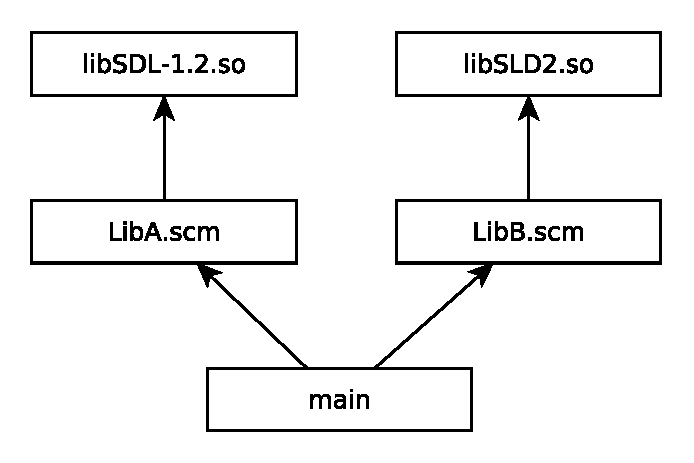
\includegraphics[width=4cm]{figures/SchemeLibrary}
%     \caption{Scheme}
%     \label{fig:1}
%   \end{center}
% \end{figure}
%%
%%Voici une insertion de plusieurs figures:
%%\begin{figure}[ht]
%%  \begin{center}
%%    \subfigure[Un cercle.]{\label{fig:2} \includegraphics[angle=-90,
%%      width=2.9cm]{figures/cercle}} \hspace{2cm}
%%    \subfigure[Un carré.]{\label{fig:3} \includegraphics[angle=-90,
%%      width=2.9cm]{figures/carre}}
%%    \caption{Des figures}
%%    \label{fig:4}
%%  \end{center}
%%\end{figure}

%%--------------%
%%     index    %
%%--------------%

%% S'il y a lieu, décommenter la ligne pour mettre votre index

%%\printindex

%%------------------------------------------------- %
%%         références --- bibliographie             %
%%------------------------------------------------- %

\nocite{*}
\bibliographystyle{plain-fr}
\bibliography{references.bib}

%\begin{thebibliography}{DDDD}
%
%\bibitem[A]{ams:guide}
%  {\scshape American Mathematical Society},
%  \emph{\AmS\LaTeX{} Version 1.1 User's Guide},
%  Amer. Math. Soc., Providence, R.~I., 1991.
%
%\bibitem[GMS]{latex2e:1}
%{\scshape M. Goossens, F. Mittelbach, and A. Samarin},
%\emph{The \LaTeX{} companion},
%Addison-Wesley, USA, 1994.
%
%\bibitem[H]{hahn:everyone}
%{\scshape J. Hahn},
%\emph{\LaTeX{} for Everyone: A reference guide and tutorial for
%    typesetting documents using a computer},
%     Personal \TeX, Inc., Mill Valley, CA., 1991.
%
%\bibitem[L]{lamport:latex}
%{\scshape Leslie Lamport},
%\emph{\LaTeX{} -- A Document Preparation System},
%     Addison-Wesley, Reading, Mass., 1986.
%
%\bibitem[M]{mckay:sty}
%{\scshape W. McKay},
%\emph{udemmem-l.sty}, fichier \LaTeX,  rédigé pour le compte de
%l'Université de Montréal, 1993.
%
%\bibitem[S]{spivak:joy}
%{\scshape M. D. Spivak},
%\emph{The Joy of \TeX{}}, second edition,
%     Amer. Math. Soc., Providence, R.~I., 1990.
%
%\bibitem[T]{latex2e:2}
%{\scshape \TeX{} User Group},
%\emph{\LaTeX2e for classand package writers},
%1995, disponible sur le web.
%
%\end{thebibliography}

%%------------------------------------------------- %
%%                  Annexe A                        %
%%------------------------------------------------- %

\appendix
\chapter{Information des environnement de test}

\begin{figure}[ht]
  \centering
\begin{mplisting}{1}
Architecture:          x86_64
CPU op-mode(s):        32-bit, 64-bit
CPU(s):                4
Thread(s) per core:    1
Core(s) per socket:    4
Vendor ID:             GenuineIntel
Model name:            Intel(R) Core(TM) i7-7700K CPU @ 4.20GHz
CPU MHz:               4200.000
CPU min MHz:           800.0000
Storage:               216GB (NVME)
RAM:                   16GB
Swap:                  16GB
C Compiler             gcc (Debian 6.3.0-18+deb9u1) 6.3.0 20170516
Ethernet Speed         1Gbps
\end{mplisting}
  \caption{La spécification de la machine arctic qui est utilisé comme nœud de destination dans
  l'ensemble des tests. Cette machine, nommé \textbf{Arctic} est refroidit au liquide.}
\end{figure}

\begin{figure}[h]
  \begin{mplisting}{1}
Architecture:        armv7l
Byte Order:          Little Endian
CPU(s):              4
Thread(s) per core:  1
Core(s) per socket:  4
Vendor ID:           ARM
Model name:          Cortex-A72
CPU max MHz:         1500.0000
CPU min MHz:         600.0000
OS:                  Linux tictoc 4.19.66-v7l+ #1253 SMP
Hostname:            tictoc.iro.umontreal.ca
Storage:             26GB (sdcard)
RAM:                 2GB
Swap:                2GB
C Compiler           gcc (Raspbian 8.3.0-6+rpi1) 8.3.0
Ethernet Speed       1Gbps
\end{mplisting}
  \caption{La spécification du CPU du Raspberry Pi utilisé dans les tests.
  Cette machine se nomme \textbf{tictoc}.}
\end{figure}

\begin{figure}[h]
  \begin{mplisting}{1}
Architecture:        x86_64
CPU(s):              12
Thread(s) per core:  2
Core(s) per socket:  6
Model name:          Intel(R) Core(TM) i7-8700B CPU @ 3.20GHz
OS:                  Darwin Kernel Version 19.2.0
Hostname:            gambit.iro.umontreal.ca
Storage:             1TB (SSD)
RAM:                 8GB
Network Speed:       1Gbps
\end{mplisting}
  \caption{La spécification de la machine Gambit utilisé Avec macOS.}
\end{figure}

%
%\section{Section un de l'Annexe A}
%
%texte
%
%\chapter{Les différentes parties et leur ordre d'apparition}
%
%J'ajoute ici les différentes parties d'un mémoire ou d'une thèse ainsi
%que leur ordre d'apparition tel que décrit dans le guide de
%présentation des mémoires et des thèses de la Faculté des études
%supérieures.  Pour plus d'information, consultez le guide sur le site
%web de la facutlé (www.fesp.umontreal.ca).
%
%\begin{table}[htbp]
%  \begin{center}
%    \begin{tabular}{|lr|}\hline
%      1. les couvertures conformes & obligatoires\\
%      2. les pages de garde & obligatoires\\
%      3. la page de titre & obligatoire\\
%      4. l'identification du jury& obligatoire\\
%      5. le résumé en français et les mots clés français& obligatoires\\
%      6. le résumé en anglais et les mots clés anglais & obligatoires\\
%      8. le résumé de vulgarisation& facultatif\\
%      9. la table des matières, la liste des tableaux,\phantom{un fantome d'espace}&\\ \phantom{9. } la liste des figures & obligatoires\\
%      10. la liste des sigles, la liste des abréviations& obligatoires\\
%      11. la dédicace& facultative\\
%      12. les remerciements & facultatifs\\
%      13. l'avant-propos & facultatif\\
%      14. le corps de l'ouvrage& obligatoire\\
%      15. l'index analytique& facultatif\\
%      16. les sources documentaires & obligatoires\\
%      17. les appendices (annexes) & facultatifs\\
%      18. le curriculum vitæ & facultatif\\
%      19. les documents spéciaux & facultatifs\\\hline
%    \end{tabular}
%    \caption{Liste des parties}
%  \end{center}
%\end{table}

\end{document}
